\documentclass[11pt,reqno]{amsart}
\usepackage[T1]{fontenc}
\usepackage{lmodern}
\pdfmapfile{+lm.map}
\usepackage[utf8]{inputenc}
\usepackage{amsmath,amssymb,amsthm,mathtools}
\usepackage{mathrsfs}
\usepackage{microtype}
\usepackage[margin=1.03in]{geometry}
\usepackage{graphicx,booktabs,array}
\usepackage{xcolor}
\definecolor{linkblue}{RGB}{28,68,110}
\usepackage[colorlinks=true,linkcolor=linkblue,citecolor=linkblue,urlcolor=linkblue,bookmarksnumbered=true]{hyperref}
\hypersetup{pdftitle={An L3 bound for the trilinear Hilbert transform},pdfauthor={OpenAI}}
\newtheorem{theorem}{Theorem}[section]
\newtheorem{lemma}[theorem]{Lemma}
\newtheorem{proposition}[theorem]{Proposition}
\newtheorem{corollary}[theorem]{Corollary}
\theoremstyle{definition}
\newtheorem{definition}[theorem]{Definition}
\theoremstyle{remark}
\newtheorem{remark}[theorem]{Remark}
\newcommand{\R}{\mathbb R}
\newcommand{\C}{\mathbb C}
\newcommand{\Z}{\mathbb Z}
\newcommand{\Q}{\mathbb Q}
\newcommand{\N}{\mathbb N}
\newcommand{\T}{\mathbb T}
\newcommand{\E}{\mathbb E}
\newcommand{\Prob}{\mathbb P}
\newcommand{\1}{\mathbf 1}
\newcommand{\ip}[2]{\langle #1,#2\rangle}
\newcommand{\norm}[1]{\lVert #1\rVert}
\newcommand{\abs}[1]{\lvert #1\rvert}
\newcommand{\phys}{\mathrm{phys}}
\newcommand{\fint}{\mathop{\mathchoice{\mkern2mu\int\mkern-15mu-\mkern7mu}{\mkern2mu\int\mkern-13mu-\mkern6mu}{\mkern2mu\int\mkern-11mu-\mkern5mu}{\mkern2mu\int\mkern-9mu-\mkern4mu}}\nolimits}
\DeclareMathOperator{\supp}{supp}
\DeclareMathOperator{\dist}{dist}
\DeclareMathOperator{\diam}{diam}
\DeclareMathOperator{\rank}{rank}
\DeclareMathOperator{\spanop}{span}
\DeclareMathOperator{\sgn}{sgn}
\setlength{\emergencystretch}{1.5em}
\allowdisplaybreaks[2]
\pdfgentounicode=1
\input{glyphtounicode}

\title[The trilinear Hilbert transform on three $L^3$ inputs]{An $L^3$ bound for the trilinear Hilbert transform}
\author{OpenAI}
\date{October 5, 2026}
\subjclass[2020]{42B20, 42B25, 11B30}
\keywords{Trilinear Hilbert transform, quadratic phases, Gowers norms, multilinear singular integrals}
\begin{document}
\begin{abstract}
We prove that the trilinear Hilbert transform with fixed slopes $1,2,3$ maps
$L^3(\R)\times L^3(\R)\times L^3(\R)$ to $L^1(\R)$, resolving this case of
the trilinear Hilbert transform conjecture.
\end{abstract}
\maketitle
\tableofcontents
\section{Introduction}\label{sec:introduction}
For Schwartz functions $f_1,f_2,f_3:\R\to\C$, set
\[
T(f_1,f_2,f_3)(x)
 =\operatorname{p.v.}\int_{\R}
 f_1(x-t)f_2(x-2t)f_3(x-3t)\,\frac{dt}{t}.
\]
The principal value removes a symmetric interval about the origin.
Our main result is the following estimate.

\begin{theorem}\label{thm:main}
There is a finite constant $C$ such that
\[
 \norm{T(f_1,f_2,f_3)}_{L^1(\R)}
 \le C\prod_{j=1}^3\norm{f_j}_{L^3(\R)}
 \qquad(f_1,f_2,f_3\in\mathcal S(\R)).
\]
Consequently $T$ has a unique bounded trilinear extension from
$L^3(\R)\times L^3(\R)\times L^3(\R)$ to $L^1(\R)$.
\end{theorem}

Theorem~\ref{thm:main} resolves affirmatively the
$L^3\times L^3\times L^3\to L^1$ case of the standard trilinear
Hilbert transform conjecture for the fixed slopes $1,2,3$.
The full conjecture asks for a broader range of exponents; see
\cite[Conjecture~1.7]{HuLie2023}.
The result here concerns the displayed fixed operator.

The bilinear predecessor was treated by Lacey and Thiele~\cite{LT1997,LT1999}.
The difficulty in the trilinear setting is the interaction of cancellation across scales with
quadratic modulation.  For example, if
$c=(-1,3,-3,1)$, then
\[
 \sum_{j=0}^3c_j(x+jt)^a=0\qquad(a=0,1,2).
\]
Thus matched quadratic phases can persist in the associated four-linear
form.  Quantitative information at one scale must be organized so that
this persistence does not produce a loss proportional to the number
of scales.
Tao~\cite{Tao2015} obtained cancellation for truncated multilinear
Hilbert transforms, improving the elementary logarithmic truncation
bound to a sublogarithmic one.  That argument established a connection
with higher-order uniformity.  The straight-line trilinear boundedness
problem remained open in the account of Hu and Lie~\cite[Section~1.2]{HuLie2025}.
Their results for curved transforms~\cite{HuLie2023,HuLie2025} address
a different source of oscillation.

The inverse theorem of Leng, Sah and Sawhney~\cite[Theorem~1.2]{LSS2024}
provides the quantitative structural input used below.  We use its
degree-two case and prove the continuous chart and localization
statements needed for the singular integral.  The inverse theorem alone
does not sum the scales.  The proof of that summation has three main
features.

First, private orthogonal coordinates make the coefficients of each
selected column recoverable.  Lemma~\ref{lem:compression} then controls
products of inherited projections uniformly in spatial depth.  Its loss
is a power of the logarithm of a common budget for column sizes, inverse
private-coordinate sizes, and the number of available labels along a
spatial path; the total number of labels on disjoint branches is unrestricted.

Second, we localize curvature jointly in all four arguments and retain
the separation needed when projection adjoints are evaluated on earlier
cells.  Transferring complementary filters leaves coupled narrow
bands.  The comparison in Lemma~\ref{lem:short-block} gives a
power of block length whose exponent tends to zero as the auxiliary
exponent decreases to two.  This control is essential to the final
absorption.

Third, each matched column receives one fixed mode expansion.
Frequency graphs separate errors with square-summable energy from
coherent components with hereditary representatives.
Lemma~\ref{lem:finite-sparse-count} bounds the total mass of progression
tests on scales of small density, with a positive-power saving in the
density.  Its application uses all four anchor cancellations and
polynomial dimension costs.  The compression and counting lemmas isolate
tools for other progression forms with the same projection and
cancellation structures.

\subsection*{Organization and notation}
Section~\ref{sec:outer} reduces the operator estimate to a uniform
maximal-function bound for local forms.  Sections~\ref{sec:compression}
and~\ref{sec:charts} develop the projection and quadratic tools.
Section~\ref{sec:base} produces a pair-small base form with a bounded
number of active scales on each path.  Section~\ref{sec:localization}
localizes this form by curvature.  Section~\ref{sec:sides} gives the side
estimates under a square-energy hypothesis, which is proved in
Section~\ref{sec:linearization}.  Section~\ref{sec:counting} estimates the
remaining core terms.  Section~\ref{sec:completion} chooses the parameters
and completes the absorption.

We write $e(t)=\exp(2\pi i t)$ and use progression coordinates
$y_j=x+jt$, $0\le j\le3$.
Inner products are linear in the first argument.  Replacing the shifts
$x-jt$ by $x+jt$ in the principal-value integral changes the operator's
sign, by the substitution $t\mapsto-t$.
Norms and inner products carrying an interval
subscript use normalized Lebesgue measure on that interval.  Other
function norms use ordinary Lebesgue measure.  In vector-valued
arguments the scalar component entering the form is called the physical
component.  All depth trees used in the estimates are finite; constants
will be uniform in their depth.  The polynomial and quasipolynomial
budget conventions are specified in Section~\ref{sec:compression}.

\section{Local forms and the outer reduction}\label{sec:outer}
Fix a dyadic lattice on $\R$.  The depth increases by one when the interval
length is halved.  For an interval $I$ of length $r$, define
\[
 H_I(z_0,z_1,z_2,z_3)
 =r^{-2}\int_{\R^2}w_I(x,t)\prod_{j=0}^3z_j(x+jt)\,dx\,dt.
\]
We fix constants $c_0>0$ and $C_0\ge1$ and call a kernel admissible when
it has the following properties:
\begin{enumerate}
\item Its support consists of points for which all four $x+jt$ lie in
$I$ at distance at least $c_0r$ from its endpoints.
\item For every $u\in\R$ and every $j\in\{0,1,2,3\}$,
\[
 \int_{\R}w_I(u-jt,t)\,dt=0.
\]
\item Every derivative of total order $n$ is bounded in absolute value by
$r^{-n}(C_0(n+2))^{C_0(n+2)}$.
\end{enumerate}
Kernels at different intervals may be chosen independently and may be
multiplied by unimodular scalars.  Constants in the proof may depend on
these fixed admissibility parameters.  For vector-valued functions the
form uses only their physical scalar components.

\begin{lemma}[Local absolute estimate]\label{lem:local-absolute}
If $p_j\ge1$ and $\sum_{j=0}^3p_j^{-1}\le2$, then
\[
 r^{-2}\int |w_I(x,t)|\prod_{j=0}^3\norm{z_j(x+jt)}\,dx\,dt
 \lesssim\prod_{j=0}^3\norm{z_j}_{p_j,I}.
\]
\end{lemma}
\begin{proof}
For distinct indices $i,j$, the map $(x,t)\mapsto(y_i,y_j)$ has
nonzero constant determinant.  The estimate follows immediately when
$p_i=p_j=1$ and the other two exponents are infinity.  The estimate with
all exponents infinity follows from the support and kernel bounds.
The endpoints with just one exponent equal to one follow from the
two-exponent bounds and normalized norm monotonicity.
Interpolation, or log-convexity applied to this positive form, fills the
polytope $0\le p_j^{-1}\le1$, $\sum p_j^{-1}\le2$.
\end{proof}

Let $M$ be the uncentered Hardy--Littlewood maximal operator and put
$M_qf=(M(|f|^q))^{1/q}$.  For $2<q<3$, let $C_N=C_N(q)$ be the least
constant such that
\[
 \sum_{I\in\mathcal I}|I|\,|H_I(f_0,f_1,f_2,f_3)|
 \le C_N\int_{\R}\prod_{j=0}^3 M_qf_j
\]
for every finite collection $\mathcal I$ in at most $N$ consecutive
depths, every lattice, every admissible kernel family, and compactly
supported $L^q$ inputs.  Lemma~\ref{lem:local-absolute}, with all
exponents two, gives $C_N\lesssim N$.  Indeed the local $L^2$ norms
are at most the local $L^q$ norms, whose product is at most
$\prod_jM_qf_j$ at every point of $I$; sum over disjoint intervals at
each depth.

\begin{theorem}[Uniform local estimate]\label{thm:local}
For some $q\in(2,3)$, the constants $C_N(q)$ are bounded independently
of $N$.
\end{theorem}

It is useful to isolate the normalized assertion that will be proved
in Section~\ref{sec:completion}.  A rooted subtree contains all
ancestors between each of its cells and its root; the summation may use
any subset of those cells.

\begin{proposition}[Normalized absorption estimate]\label{prop:normalized}
For a suitable fixed $q\in(2,3)$ and every sufficiently small fixed
$c>0$, there is an $A<\infty$, independent of $N$, with the following
property.  Suppose a finite rooted subtree has root $I_*$, all summation
cells lie in at most $N$ consecutive depths, and
\[
 \norm{f_j}_{q,I}\le1
 \qquad(0\le j\le3, I\text{ in the subtree}).
\]
Then
\[
 \sum_{I\text{ a summation cell}}|I|\,|H_I(f)|
 \le (A+cC_N)|I_*|.
\]
\end{proposition}

The rest of the proof establishes Proposition~\ref{prop:normalized}.
At this stage $C_N$ is finite, with the preliminary bound $C_N\lesssim N$.
The constant $A$ may depend on the fixed choices of $q$, $c$, and the
accuracy parameters, but is independent of $N$.  The stopping argument
below gives $C_N\le C A+C cC_N$; choosing $c$ sufficiently small then
gives the uniform bound.  Thus the long construction needs a small
coefficient of the finite constant $C_N$, which will be absorbed only
after Proposition~\ref{prop:normalized} is proved.

\begin{lemma}[Outer reduction]\label{lem:outer}
Proposition~\ref{prop:normalized} implies Theorem~\ref{thm:local},
and Theorem~\ref{thm:local} implies Theorem~\ref{thm:main}.
\end{lemma}
\begin{proof}
We first remove the normalization.  Start with disjoint roots at the
largest interval size occurring in the finite collection.  At a root
$J$, put $a_{j,J}=\norm{f_j}_{q,J}$.  A zero root size gives zero
contribution below that root.  Otherwise stop at the first strict
descendants $J'$ for which one average of $|f_j|^q$ exceeds
$16a_{j,J}^q$.  For each fixed $j$ the union of its first stops has length
at most $|J|/16$, so the union of all stops has length at most $|J|/4$.
On the intervening tree, division of $f_j$ by $16^{1/q}a_{j,J}$ makes
all required local sizes at most one.  Proposition~\ref{prop:normalized}
therefore bounds this tree by
\[
 16^{4/q}(A+cC_N)|J|\prod_ja_{j,J}.
\]
Repeat at the stopped roots.  The sets
$E_J=J\setminus\bigcup J'$ are disjoint over this recursive family,
have measure at least $3|J|/4$, and satisfy
$M_qf_j(x)\ge a_{j,J}$ for $x\in E_J$.  Hence
\[
 \sum_J |J|\prod_ja_{j,J}
 \le\tfrac43\int\prod_jM_qf_j.
\]
Taking the supremum gives
$C_N\le C A+C cC_N$, where $C$ is bounded uniformly for $2<q<3$.
Choose $c$ so that $Cc<1/2$ and absorb.  This proves
Theorem~\ref{thm:local}.

To recover the continuous kernel, take an odd compactly supported
Gevrey function $\phi$ with $\phi^{(3)}(0)\ne0$, and a compactly
supported Gevrey function $\omega$ such that
$\sum_{m\in\Z}\omega(X-m)=1$.  Set
\[
 W(X,S)=\prod_{j=0}^3(\partial_S-j\partial_X)
                 [\omega(X)\phi(S)].
\]
Each factor is differentiation in the direction of integration on the
corresponding line $X=u-jS$.  Compact support therefore makes all four
one-point marginals of $W$ vanish.  Spatial summation and a change of
variables give
\[
 \sum_{m\in\Z}W(x/a-m,t/a)=\phi^{(4)}(t/a),\qquad
 \int_0^\infty\phi^{(4)}(t/a)\,\frac{da}{a^2}
 =-\frac{\phi^{(3)}(0)}{t}\quad(t\ne0).
\]
For the second equality one first takes $t>0$ and substitutes $s=t/a$;
for $t<0$ use oddness of $\phi^{(4)}$.

Write $a=b2^n$, $1\le b<2$.  For each fixed $b$, a kernel
$a^{-1}W(x/a-m,t/a)$ can be put into the form $r^{-1}w_I(x,t)$ with
$r=Da$ for a fixed sufficiently large dyadic $D$.  To choose $I$, use
a fixed finite family of shifted lattices.  At scale $r$ their
boundaries may be placed at offsets $0,r/3,-r/3$, with alternating signs
between depths to preserve nesting.  The four progression coordinates
on the support occupy an interval of length $O(a)$; for large $D$, one
of these cells contains that interval with the fixed interior margin.
Each chosen cell receives only a bounded number of translates.  The
rescaled derivative and support bounds are fixed, so choose $c_0,C_0$
once to include them.  A bounded number of contributions at one cell
can be estimated separately.

Theorem~\ref{thm:local}, summed over these lattices, gives a uniform
bound for the absolute sum over any finite range of $n$ and the relevant
spatial translates.  Integrate in $b$ with measure $db/b$.  For compactly
supported bounded $f_0$ and Schwartz $f_1,f_2,f_3$, the resulting bound is
\[
 C\int\prod_{j=0}^3M_qf_j
 \le C_q\norm{f_0}_\infty\prod_{j=1}^3\norm{f_j}_3.
\]
Here $M_q$ is bounded on $L^3$ because $q<3$; use H\"older with the
three exponents equal to three.  Compact truncations of the other
inputs justify use of the defining class for $C_N$: at a finite range
of scales and with compact support in slot zero, every relevant
progression coordinate lies in a fixed compact set.

After spatial summation the kernel is odd.  Pair positive and negative
$t$ near zero; the difference of the two products of Schwartz functions
is $O(|t|)$ uniformly on the compact support of $f_0$.  At large $|t|$
the Schwartz bounds are integrable.  The integrated scale kernels have
absolute value at most $C/|t|$.  Dominated convergence therefore permits
the scale range to tend to all positive $a$ and recovers a nonzero
constant times the principal-value four-linear form.  Reflection of
$t$ changes only its sign and gives the operator in
Theorem~\ref{thm:main}.  Duality against compactly supported bounded
$f_0$ proves the inequality in Theorem~\ref{thm:main}.  Density of Schwartz functions,
trilinearity, and completeness of $L^1$ give the stated extension.
\end{proof}

\section{Budgets, private coordinates, and compression}
\label{sec:compression}

We first make precise the quantitative conventions and the projection estimates
used below.  All trees in this section are finite.  Bounds are independent of
their number of generations.

\subsection{Quantitative conventions and stopping attempts}

A rational number has height at most $B$ if it can be written as $p/q$ with
$p\in\Z$, $q\in\N$, and $\max(|p|,q)\le B$.  Heights of rational vectors and
matrices are entrywise heights.  For parameters $H_1,\ldots,H_s\ge e$ and
$0<\delta_1,\ldots,\delta_t\le1$, a quasipolynomial bound means a bound of the
form
\[
 \exp\!\left(C_q\left(1+\sum_{a=1}^s\log H_a
                  +\sum_{b=1}^t\log(1/\delta_b)\right)^C\right).
\]
A polylogarithmic bound is the same expression without the outer exponential.
Here and below the degrees denoted by $C$ can be fixed independently of $q$,
of spatial lengths and frequencies, and of the number of scales.  Constants
such as $C_q$ may depend on the fixed choice of $q$ and on the fixed kernel
class.  A bounded number of compositions of quasipolynomial constructions is
again quasipolynomial.  When the number of constructions is itself a parameter,
we keep track of the resulting growth explicitly.  Expressions such as
$D\le\exp(k^C)$ allow an increase of the fixed exponent and a sufficiently
large lower threshold for $k$.

We will use elementary spatial packing in the following form.  If $J$ is a
dyadic interval, $a_I\ge0$, and
\[
 \sum_{I\ni y}a_I\le A \qquad\text{for almost every }y\in J,
\]
where all the intervals in the sum are contained in $J$, then Tonelli's
theorem gives
\[
 \sum_I |I|a_I
   =\int_J\sum_{I\ni y}a_I\,dy\le A|J|.
\]
This is the passage from a bound along a spatial path to a length-weighted
tree bound.

\begin{lemma}[Packing of attempts]
\label{lem:attempt-packing}
Suppose a construction on a root $J$ sends exceptional cells and all their
descendants to new estimates on disjoint subroots.  Suppose that, at every
root $R$, the new roots $R'$ satisfy
\[
 \sum_{R'\text{ child root of }R}|R'|\le\rho |R|,
 \qquad 0\le\rho<1.
\]
Then the sum of the lengths of all roots, including $J$, is at most
$|J|/(1-\rho)$.  In particular, if the contribution assigned to an attempt
from $R$ is at most $A|R|$, with its hypotheses valid at every new root, the
total contribution is at most $A|J|/(1-\rho)$.
\end{lemma}

\begin{proof}
The sum of the root lengths in generation $n$ is at most $\rho^n|J|$, by
induction.  Summing this geometric series proves both assertions.
\end{proof}

We refer to one application of the construction at a root as an
\emph{attempt}.  Several stopping requirements can be imposed together: if
their exceptional root families cost fractions $\rho_1,\ldots,\rho_s$, take
the maximal intervals in their union.  These are disjoint, their total length
is at most $(\sum_a\rho_a)|R|$, and Lemma~\ref{lem:attempt-packing}
applies when this sum
is smaller than one.  A local normalization required by an estimate must hold
at each new root before that estimate is restarted there.

A stopping boundary for the summation does not have to be a boundary for an
auxiliary projection family.  An inherited column list can be continued on
all descendants of a terminal decision cell: retain its columns and refit
their constant coefficients on each finer cell.  This gives genuine nested
projections on the full refining partitions needed for an operator estimate.
If a later attempt uses a new family, the extension of the old family is
still used for the summands assigned to the old attempt.  In particular, a
projection on a partition refining $I$ is an $L^2(I)$ contraction whether or
not the averages of the original input are normalized on the finer cells.

\subsection{Columns and inherited projections}

Fix a finite dyadic tree with root $J$ and a finite label set $\mathcal V$.
The cardinality of $\mathcal V$ will not be bounded.  To each label $v$ assign
a birth cell $J_v\subset J$, a scalar function $\varphi_v$ on $J_v$, and a
number $\epsilon_v>0$.  Work in the value Hilbert space
\[
 \mathcal H=\C\oplus\ell^2(\mathcal V),
\]
and define the column on its birth cell by
\[
 \Phi_v(y)=\bigl(\varphi_v(y),\sqrt{\epsilon_v}\,\mathbf e_v\bigr),
 \qquad y\in J_v.
\]
The first coordinate is called the physical coordinate.  Every label has its
own private direction, even when two scalar functions $\varphi_v$ coincide.
We write $\widetilde\Phi_v=\1_{J_v}\Phi_v$ for the extension by zero to $J$.

Throughout the projection estimates, $D\ge2$ is a common budget such that
\begin{equation*}
 \|\Phi_v\|_{L^\infty(J_v;\mathcal H)}\le D,
 \qquad \sqrt{\epsilon_v}\ge D^{-1},
 \qquad \sum_{v\in\mathcal V}\1_{J_v}(y)\le D
       \quad\text{for almost every }y\in J.
\end{equation*}
The last condition says that at most $D$ labels are born along any spatial
path.  It counts all available labels, including labels not selected in the
projection currently under consideration.  It allows arbitrarily many labels
on disjoint branches.

A mask $\mathcal V^i(I)$ on a cell $I$ is a subset of
$\{v:I\subset J_v\}$.  An inherited mask family satisfies
\[
 \mathcal V^i(I)\subset\mathcal V^i(I')
 \qquad\text{whenever }I'\text{ is a child of }I.
\]
Let $P_I^i$ be the orthogonal projection in $L^2(I;\mathcal H)$ onto
\[
 \left\{\sum_{v\in\mathcal V^i(I)}c_v\Phi_v|_I:c_v\in\C\right\}.
\]
The coefficients in this definition are constant on $I$.  We also regard
$P_I^i$ as an operator on $L^2(J;\mathcal H)$ by restricting its input to $I$
and extending its output by zero.  For a stopping partition $\pi$ of a cell,
$P_\pi^i$ denotes the direct sum of these local projections.  If $\pi'$
refines $\pi$, inheritance implies
\[
 \operatorname{range}(P_\pi^i)
     \subset\operatorname{range}(P_{\pi'}^i).
\]
Indeed, the restriction of an old constant-coefficient combination to a
smaller cell is still an allowed combination there.  Thus these direct-sum
projections are nested, even though their coefficients are refitted on every
cell.  Their successive differences are orthogonal projections with mutually
orthogonal ranges.

The masks and birth lists may have been chosen using an input or previous
stopping decisions.  In each application of an operator estimate we hold the
entire resulting family fixed.

\begin{lemma}[Coefficient and projection bounds]
\label{lem:private-columns}
If $\mathcal A$ is any set of columns available on a cell $I$, then
\[
 D^{-1}\left(\sum_{v\in\mathcal A}|c_v|^2\right)^{1/2}
 \le \left\|\sum_{v\in\mathcal A}c_v\Phi_v(y)\right\|_{\mathcal H}
 \le D^{3/2}\left(\sum_{v\in\mathcal A}|c_v|^2\right)^{1/2}
 \quad\text{for almost every }y\in I.
\]
In particular, the coefficients are unique.  The orthogonal projection
$P_{I,\mathcal A}$ onto their span satisfies
\[
 \|P_{I,\mathcal A}z\|_{L^\infty(I;\mathcal H)}
       \le D^5\fint_I\|z(y)\|_{\mathcal H}\,dy.
\]
For an actual scalar input $F=(f,0)$, write
$P_{I,\mathcal A}F=\sum_{v\in\mathcal A}c_v\Phi_v$.  Then
\[
 \fint_I\bigl(f-(P_{I,\mathcal A}F)_{\phys}\bigr)
                         \overline{\varphi_v}
       =\epsilon_v c_v \qquad(v\in\mathcal A).
\]
\end{lemma}

\begin{proof}
The private component of the sum has squared norm
$\sum_v\epsilon_v|c_v|^2$, giving the lower bound.  The upper bound follows
from Cauchy--Schwarz, since there are at most $D$ columns and each has norm at
most $D$.

Let $E_y:\ell^2(\mathcal A)\to\mathcal H$ be the evaluation map
$E_yc=\sum_vc_v\Phi_v(y)$, and let
\[
 G=\fint_I E_y^*E_y\,dy
\]
be the normalized Gram matrix.  The bounds just proved give
$G\ge D^{-2}\operatorname{Id}$ and $\|E_y\|\le D^{3/2}$.  Therefore the
projection has the integral representation
\[
 P_{I,\mathcal A}z(y)
      =\fint_I E_yG^{-1}E_t^*z(t)\,dt,
 \qquad \|E_yG^{-1}E_t^*\|\le D^5.
\]
This proves the supremum estimate.  Finally, orthogonality to $\Phi_v$ says
that the physical pairing in the last assertion minus $\epsilon_vc_v$ is
zero.
\end{proof}

\subsection{A binary-prefix estimate}

The following elementary Hilbert space fact supplies the dependence on the
number of stopping generations.  In the compression argument that number
will be a power of $D$, so its logarithm is the appropriate cost.
Its proof uses the classical Rademacher--Menshov binary-decomposition
mechanism; see \cite[Section~3, Lemma~1]{MM2011} for a vector-valued
presentation.  The nested projection products and Bessel rows are treated
below.

\begin{lemma}[Products of nested prefixes]
\label{lem:projection-prefixes}
Let $\mathcal X$ be a Hilbert space, and for $1\le i\le m$ let
$P_0^i,\ldots,P_T^i$ be nested orthogonal projections on $\mathcal X$.
Set $Z_n=P_n^m\cdots P_n^1$ and
\[
 L_T=1+\left\lceil\log_2(T+1)\right\rceil.
\]
Suppose $B_\nu:\mathcal X\to\mathcal Y_\nu$ are finitely many bounded linear operators
satisfying $\sum_\nu\|B_\nu h\|^2\le\|h\|^2$.  For any choices
$n(\nu)\in\{0,\ldots,T\}$,
\[
 \left(\sum_\nu\|B_\nu Z_{n(\nu)}g\|^2\right)^{1/2}
       \le L_T^m\|g\|.
\]
Moreover,
\[
 \sum_{n=1}^T\|(Z_n-Z_{n-1})g\|^2
       \le m^2L_T^{2(m-1)}\|g\|^2
       \le m^2L_T^{2m}\|g\|^2.
\]
For $m=0$ the product is the identity and the first estimate has constant one.
\end{lemma}

\begin{proof}
Put $\Delta_0^i=P_0^i$ and $\Delta_n^i=P_n^i-P_{n-1}^i$ for $n\ge1$.
Within each family these are pairwise orthogonal projections.  A prefix of
the index set $\{0,\ldots,T\}$ can be partitioned into dyadic index blocks,
with at most one block of each length.  For a block $A$ put
$\Delta_A^i=\sum_{n\in A}\Delta_n^i$.  At any fixed block length, the
operators $\Delta_A^i$ are pairwise orthogonal projections.

Expand each factor of $Z_{n(\nu)}$ using this binary decomposition.  Fix a
tuple of block lengths, one for each of the $m$ factors.  A term is zero if
one of those lengths does not occur in the relevant prefix.  Otherwise it
has the form
\[
 B_\nu\Delta_{A_m(\nu)}^m\cdots\Delta_{A_1(\nu)}^1g.
\]
Group rows with the same tuple of blocks.  The row contraction bounds their
sum of squared norms by
$\|\Delta_{A_m}^m\cdots\Delta_{A_1}^1g\|^2$.  Summing over the block
tuples that occur is bounded by the sum over all tuples of those fixed
lengths.  Successive Bessel inequalities give
\[
 \sum_{A_1,\ldots,A_m}
       \|\Delta_{A_m}^m\cdots\Delta_{A_1}^1g\|^2\le\|g\|^2.
\]
This argument uses orthogonality within each layer, not commutation between
layers.  There are at most $L_T^m$ tuples of block lengths.  The triangle
inequality in the Hilbert direct sum of the row spaces proves the first
assertion.

For the second, telescope in the order
\[
 Z_n-Z_{n-1}
   =\sum_{i=1}^m
       P_n^m\cdots P_n^{i+1}\Delta_n^i
                       P_{n-1}^{i-1}\cdots P_{n-1}^1.
\]
Discard the left contractions and use Cauchy--Schwarz in the sum over $i$.
For a fixed $i$, the rows $B_n=\Delta_n^i$, $1\le n\le T$, satisfy the row
contraction hypothesis.  Apply the first assertion to the $i-1$ preceding
families and the prefix index $n-1$.  The resulting bound is
\[
 \sum_{n=1}^T\|(Z_n-Z_{n-1})g\|^2
    \le m\sum_{i=1}^m L_T^{2(i-1)}\|g\|^2
    \le m^2L_T^{2(m-1)}\|g\|^2,
\]
as claimed.
\end{proof}

\subsection{Compression of local projection products}

\begin{lemma}[Compression]
\label{lem:compression}
Use the column system and budget $D\ge2$ above on a finite dyadic tree with
root $J$.  Let $P^1,\ldots,P^m$ be inherited mask families, with their local
orthogonal projections.  Suppose finitely many bounded linear rows
\[
 B_\nu:L^2(J;\mathcal H)\longrightarrow\mathcal Y_\nu
\]
satisfy
\[
 \sum_\nu\|B_\nu z\|_{\mathcal Y_\nu}^2\le\|z\|_{L^2(J;\mathcal H)}^2,
 \qquad B_\nu=B_\nu\1_{u(\nu)},
\]
where each $u(\nu)$ is a cell of the tree.  Then an absolute constant $C$
satisfies
\[
 \left(\sum_\nu
    \|B_\nu P_{u(\nu)}^m\cdots P_{u(\nu)}^1z\|^2\right)^{1/2}
 \le \bigl(C(m+1)^C\log(2D)\bigr)^{C(m+1)}\|z\|_{L^2(J;\mathcal H)}.
\]
The estimate is uniform in the row cells, the total number of labels, and the
number of spatial depths.  Identity factors may be omitted.  Products
containing complements $1-P^i$ satisfy the same form of bound after changing
$C$.  Integrating such compositions against a fixed finite measure costs, in
addition, at most the total variation of that measure.
\end{lemma}

\begin{proof}
For a nonempty product, we first divide the row cells into size segments
and, on each segment, replace the input by a bounded function with the
same first-layer moments.  We then stop when the last-layer coefficient
vector moves: nested-prefix estimates control the anchor products, and
the pathwise birth-label budget controls the coefficient errors.
Attempts are summed using both length and energy contraction.  Finally,
the size segments are summed using the bounds for their weighted
averages and representative energies.

The assertion for an empty product is the row contraction hypothesis.  Assume
$m\ge1$, and abbreviate the ordinary $L^2(J;\mathcal H)$ norm to $\|\cdot\|_2$.
Add one final dyadic generation below all row cells, retaining columns and
refitting there if necessary.  This changes neither the hypothesis nor the
quantity to be estimated.

\paragraph{Size segments and a bounded moment representative.}
For every cell $K$ put
\[
 a_K=\fint_K\|z(y)\|_{\mathcal H}\,dy.
\]
Starting from $J$, stop at the first proper descendant cells for which the
average is greater than $2a_J$, and repeat inside each stopping cell.  It is
enough to run this stopping rule through the last possible row depth.  A root
with zero average contributes no rows and can be omitted.  Denote the
resulting stopping roots by $\mathcal S$.

Assign a row cell $u$ to the deepest root $K\in\mathcal S$ containing it.
More generally, let $\mathcal T_K$ be the full subtree of cells in $K$ that
are not contained in a proper stopping child of $K$, through the last row
depth.  Thus every assigned row cell lies in $\mathcal T_K$.  Cut $K$ at its
next stopping roots and at final leaves on all other paths; denote this
partition by $\pi_K$.  Every assigned row cell is partitioned by cells of
$\pi_K$.  On a cut cell $Q$ the average of $\|z\|$ is at most $4a_K$: its
dyadic parent has average at most $2a_K$, and a child average is at most twice
its parent's average.

For $Q\in\pi_K$, take all first-layer labels used by cells of
$\mathcal T_K$ containing $Q$, and project $z|_Q$ onto their restrictions to
$Q$.  Let $g_K$ be the direct sum of these projections, extended by zero off
$K$.  At most $D$ labels occur on each such path.  By
Lemma~\ref{lem:private-columns}, with
\[
 G=4D^5,
\]
we have
\[
 \|g_K\|_{L^\infty(K;\mathcal H)}\le Ga_K,
 \qquad \|g_K\|_2^2=\langle z,g_K\rangle.
\]
The second identity follows from orthogonality on each cut cell.  If
$u\in\mathcal T_K$ and $v\in\mathcal V^1(u)$, then $v$ was included on
every cut cell inside $u$.  Adding its moment identities over that partition
of $u$ gives
\[
 P_u^1g_K=P_u^1z,
 \qquad P_u^m\cdots P_u^1g_K=P_u^m\cdots P_u^1z.
\]

Let $M_{\mathrm d}\|z\|$ be the dyadic maximal function within $J$.
Stopping averages more than double on every path.  Consequently
\[
 \sum_{K\in\mathcal S}a_K^2|K|
    \le\frac43\|M_{\mathrm d}\|z\|\|_2^2
    \le\frac{16}{3}\|z\|_2^2.
\]
We also need the stronger bound for the moment representatives
\[
 S:=\sum_{K\in\mathcal S}\|g_K\|_2^2
       \le C\log(2D)\|z\|_2^2.
\]
Here is a proof that avoids any factor which is a power of $D$.  At a fixed
point $y$, split the roots containing $y$ according as
\[
 a_K<\frac{M_{\mathrm d}\|z\|(y)}{GD^2}
 \quad\text{or}\quad
 a_K\ge\frac{M_{\mathrm d}\|z\|(y)}{GD^2}.
\]
The sum of $a_K$ in the first class is at most twice its displayed upper
threshold.  Thus their total pointwise contribution to
$\sum_K\|g_K(y)\|$ is at most $2D^{-2}M_{\mathrm d}\|z\|(y)$.  The second
class has at most
\[
 L_D=2+\left\lceil\log_2(GD^2)\right\rceil\le C\log(2D)
\]
members, since $a_K\le M_{\mathrm d}\|z\|(y)$ and the averages double.
Using the moment identity, pointwise Cauchy--Schwarz for the second class,
and then Cauchy--Schwarz in $y$, we obtain
\[
 S\le 2D^{-2}\|z\|_2\|M_{\mathrm d}\|z\|\|_2
          +\sqrt{L_D}\,\|z\|_2\sqrt S
   \le4D^{-2}\|z\|_2^2+\sqrt{L_D}\,\|z\|_2\sqrt S.
\]
Solving this quadratic inequality in $\sqrt S$ proves the asserted bound.

\paragraph{Anchors within one size segment.}
Fix $K\in\mathcal S$, write $g=g_K$ and $a=a_K$, and put
\[
 \tau=D^{-10},\qquad
 b=2D(m+1),\qquad
 T=\left\lceil b^{128(m+1)^2}\right\rceil.
\]
For each cell $u\in\mathcal T_K$, let $c(u)$ be the unique last-layer
coefficient vector of $P_u^m\cdots P_u^1g$, extended by zero to all labels.

We describe an attempt from a cell $R\in\mathcal T_K$, initially $R=K$.
Declare $R$ an anchor.  From an anchor $A$, choose as its next anchors the
first proper descendant cells $u\in\mathcal T_K$ for which
\[
 \|c(u)-c(A)\|_{\ell^2(\mathcal V)}>\tau a.
\]
Stop a path at its $T$th transition and send that cell and its descendants
to a new attempt, using the same $g$ and $a$.  Denote the disjoint new roots
from $R$ by $\mathcal R(R)$.

To apply Lemma~\ref{lem:projection-prefixes}, complete each anchor generation
to a stopping partition $\pi_n$ of $R$, $0\le n\le T$.  The active atoms are
the anchors of generation $n$.  The other atoms are terminal cut cells on
paths that have ended; leave those atoms unchanged in later partitions.
When refining an active anchor, its next anchors together with the terminal
cut cells not lying inside a next anchor partition it.  Use the original
masks on active anchors.  On a terminal cut one can use an inherited local
refit, for example with its original mask if that mask is already defined,
and keep this local projection unchanged afterward.  Hence these are
refining partitions, and the resulting direct-sum auxiliary projection
families $P_n^i=P_{\pi_n}^i$ are nested.  Put
$Z_n=P_n^m\cdots P_n^1$ on $L^2(R;\mathcal H)$.

For any $R'\in\mathcal R(R)$, its ancestors in the anchor tree have
generations $0,\ldots,T$.  On $R'$ the restriction of
$(Z_n-Z_{n-1})(\1_Rg)$ is the difference of the constant-coefficient
combinations at the corresponding two consecutive anchors.  Inheritance
makes all the older labels available at the newer anchor.  The private
coordinate bound in Lemma~\ref{lem:private-columns} therefore gives
\[
 \|(Z_n-Z_{n-1})(\1_Rg)(y)\|_{\mathcal H}
         >D^{-1}\tau a
 \quad\text{for almost every }y\in R',\quad 1\le n\le T.
\]
Integrating over the disjoint new roots, summing in $n$, and applying
Lemma~\ref{lem:projection-prefixes} yields
\[
 T D^{-2}\tau^2a^2\sum_{R'\in\mathcal R(R)}|R'|
        \le m^2L_T^{2m}\|\1_Rg\|_2^2.
\]
Since $\|g\|_\infty\le Ga$, this implies both
\[
 \sum_{R'\in\mathcal R(R)}|R'|\le E|R|,
 \qquad
 \sum_{R'\in\mathcal R(R)}\|\1_{R'}g\|_2^2
       \le E\|\1_Rg\|_2^2,
 \qquad
 E=\frac{16D^{32}m^2L_T^{2m}}{T}.
\]
Our fixed choice of $T$ makes $E<1/2$.  For completeness, $b\ge8$ and
\[
 L_T\le129(m+1)^2\log_2 b\le b^4.
\]
The second inequality follows from $m+1\le b/4$ and
$\log_2b\le b/2$.  Thus
\[
 E\le16b^{34+8m-128(m+1)^2}
       \le16\,8^{-470}<\tfrac12.
\]
It follows by generation-by-generation summation that all attempt roots
inside this size segment, denoted by $\mathcal R_K$, satisfy
\[
 \sum_{R\in\mathcal R_K}|R|\le2|K|,
 \qquad
 \sum_{R\in\mathcal R_K}\|\1_Rg_K\|_2^2\le2\|g_K\|_2^2.
\]

\paragraph{Rows assigned to an attempt.}
Assign a row in the size segment to the deepest attempt root containing its
cell.  For a row cell $u$ assigned to the attempt from $R$, let $A$ be its
last ancestor anchor in that attempt, and let $j$ be the generation of $A$.
Here $0\le j<T$.  The cell $A$ is an atom of $\pi_j$ and contains $u$.
Consequently the restriction of $Z_j(\1_Rg_K)$ to $u$ is exactly the product
at the anchor, restricted to $u$.  The stopping rule gives
\[
 \|c(u)-c(A)\|_{\ell^2(\mathcal V)}\le\tau a_K.
\]
The support condition on $B_\nu$ now permits the decomposition of its input
product into this anchor product and its coefficient error.  The rows
assigned to $R$, restricted to $L^2(R;\mathcal H)$, still satisfy the row
contraction hypothesis.  Lemma~\ref{lem:projection-prefixes} shows that their
anchor contributions have squared sum at most
\[
 L_T^{2m}\|\1_Rg_K\|_2^2.
\]
This is the step in which arbitrary, unequal physical depths of the row
cells cause no additional cost: the prefix index is the row's last anchor
generation, and its cell lies wholly in that anchor atom.

For the error write $e_{\nu,v}=c(u(\nu))_v-c(A(\nu))_v$.  It is supported
on labels available on $u(\nu)$ and has squared coefficient sum at most
$\tau^2a_K^2$.  Since $u(\nu)\subset R\cap J_v$ whenever this coefficient
can be nonzero, locality of $B_\nu$ gives
\[
 B_\nu\left(\1_{u(\nu)}\sum_ve_{\nu,v}\Phi_v\right)
       =\sum_ve_{\nu,v}B_\nu(\1_R\widetilde\Phi_v).
\]
Cauchy--Schwarz in $v$, followed by the row contraction for each fixed
label, bounds the squared sum of errors in this attempt by
\begin{align*}
 &\tau^2a_K^2
     \sum_v\sum_{\substack{\nu\text{ assigned to }R\\
                            v\text{ available on }u(\nu)}}
           \|B_\nu(\1_R\widetilde\Phi_v)\|^2 \\
 &\hspace{20mm}\le
      \tau^2a_K^2\sum_v\|\1_R\widetilde\Phi_v\|_2^2
      \le\tau^2a_K^2D^3|R|.
\end{align*}
The last inequality uses the pathwise budget in its integral form:
\[
 \sum_v\|\1_R\widetilde\Phi_v\|_2^2
   =\int_R\sum_{v:y\in J_v}\|\Phi_v(y)\|_{\mathcal H}^2\,dy
   \le D^3|R|.
\]
In particular, no estimate of the total number of labels on different
branches has been used.

\paragraph{Summation and the final constant.}
Each row belongs to exactly one size segment and one attempt within it.
The triangle inequality in the full row Hilbert space, the two packing
bounds, and the estimates for $S$ and the stopping averages give
\begin{align*}
 \left(\sum_\nu
     \|B_\nu P_{u(\nu)}^m\cdots P_{u(\nu)}^1z\|^2\right)^{1/2}
 &\le
    L_T^m\left(2\sum_K\|g_K\|_2^2\right)^{1/2}
    +\tau D^{3/2}
          \left(2\sum_Ka_K^2|K|\right)^{1/2} \\
 &\le C\left(L_T^m\sqrt{\log(2D)}+D^{-17/2}\right)\|z\|_2.
\end{align*}
Finally,
\[
 L_T\le C(m+1)^2\log(2D(m+1))
       \le C(m+1)^3\log(2D),
\]
which is bounded by the stated expression after increasing its absolute
constant.  A complement is expanded as $1-P^i$; the at most $2^m$ resulting
ordered products obey the same form of bound, and their number is absorbed
in that constant.  For a fixed average of compositions, apply the estimate
to each member and use the integral triangle inequality in the row Hilbert
space.  This proves the remaining assertions.
\end{proof}

\subsection{Rational heights and occupied scale ranges}

The next observation is useful when real frequencies are unrestricted but
all coefficients used to combine them have bounded rational height.  Small
divisors can place the relevant scale ranges far apart; they do not create
arbitrarily many such ranges.

\begin{lemma}[Height bins]
\label{lem:height-bins}
Let $d\ge1$, $B\ge2$, and $\xi\in\R^d$.  Let
\[
 \mathcal E=\left\{|a\cdot\xi|:
       a\in\Q^d\text{ has height at most }B,\ a\cdot\xi\ne0\right\}.
\]
There is an absolute constant $C$ such that the following assertions hold.
\begin{enumerate}
\item The set $\{\log_2v:v\in\mathcal E\}$ is contained in a union of at
most $d$ intervals, each of length at most
$C(d+1)^3\log(2B)$.  In particular, $\mathcal E$ meets at most
$C(d+1)^4\log(2B)$ dyadic magnitude bins.
\item If $r_n=r_0 2^{-n}$ with $r_0>0$, $\ell\in\{1,2\}$, and
$0<\alpha\le\beta$, then
\[
 \#\{n\in\Z:\text{ some }v\in\mathcal E
                  \text{ satisfies }\alpha\le r_n^\ell v\le\beta\}
 \le C(d+1)^4\bigl(\log(2B)+\log(2\beta/\alpha)\bigr).
\]
\item For every $\varepsilon>0$, with the maximum of an empty set defined
to be zero,
\[
 \sum_{n\in\Z}
     \max\bigl(\{r_n^\ell v:v\in\mathcal E,
                       r_n^\ell v\le\varepsilon\}\cup\{0\}\bigr)
     \le C(d+1)^4\log(2B)\,\varepsilon.
\]
\end{enumerate}
The same conclusions apply to suprema of finitely many such coordinate
evaluations.  For Euclidean norms of evaluation vectors with at most $h$
coordinates, one can add $C d\log(2h)$ to the bounds for the number of
occupied bins and scales, and to the coefficient of $\varepsilon$ in the
last estimate.  No bound on the size of $\xi$ is required.
\end{lemma}

\begin{proof}
If $\mathcal E$ is empty there is nothing to prove.  It is otherwise a
finite set.  We first bound coefficients in a minimal rational dependence.
Suppose $a_1,\ldots,a_k$ are minimally dependent vectors of the indicated
height.  Then $k\le d+1$ and their rank is $k-1$.  For each $i$, clear the
denominators in its $d$ entries by a common denominator $q_i\le B^d$.
The integer vector $v_i=q_i a_i$ has each entry bounded by $B^d$.  Select
$k-1$ coordinate rows on which the vectors have rank $k-1$.  Their signed
maximal minors give a null vector $(b_1,\ldots,b_k)$ with
\[
 0<|b_i|\le d! B^{d^2}.
\]
None of these minors is zero: a zero component of a null vector would give
a dependence on a proper subset, contrary to minimality.  Returning to
the original vectors gives
\[
 \sum_{i=1}^k c_i a_i=0,
 \qquad c_i=b_iq_i\in\Z\setminus\{0\},
 \qquad |c_i|\le H:=d! B^{d^2+d}.
\]

Set $R=4dH$.  Suppose coefficient vectors have nonzero evaluation magnitudes
\[
 0<s_1<s_2<\cdots<s_k,
 \qquad s_{i+1}>Rs_i.
\]
If these vectors were dependent, apply the preceding construction to a
minimal dependent subset, ordered by evaluation magnitude, and let $s_*$
be its largest magnitude.  The coefficient of that term has absolute value
at least one, whereas all the other terms together have absolute value at
most
\[
 dH\frac{s_*}{R}<s_*.
\]
They cannot sum to zero.  Thus vectors whose evaluation magnitudes are
successively separated by a factor greater than $R$ are linearly
independent, and there can be at most $d$ of them.

Choose the smallest element $s$ of $\mathcal E$, cover $[s,Rs]$, and repeat
with the smallest still uncovered element.  The selected elements are
successively separated by more than $R$, so at most $d$ intervals are
needed.  Their logarithmic lengths are $\log_2R$, and
\[
 \log_2R
    \le C(d+1)^2\log(2dB)
    \le C(d+1)^3\log(2B).
\]
Each logarithmic interval meets at most $2+\log_2R$ unit bins.  This proves
the first assertion.

For the second, consider one logarithmic value interval $[s,s+\log_2R]$.
The condition $\alpha\le r_n^\ell v\le\beta$ confines $n$ to a real
interval of length at most
\[
 \frac{\log_2R+\log_2(\beta/\alpha)}{\ell}.
\]
That interval has at most two plus its length integer points.  Summing over
the at most $d$ value intervals and using the preceding bounds proves the
claimed scale count.  The factor $r_0$ translates the interval and has no
effect on its length.

For the third, partition $\mathcal E$ by its occupied bins
$[2^j,2^{j+1})$.  For one such bin, a contribution at scale $n$ is possible
only if $r_n^\ell2^j\le\varepsilon$, and its maximum is at most
$r_n^\ell2^{j+1}$.  Let $n_0$ be the first integer for which the former
inequality holds.  The sum of these upper bounds for $n\ge n_0$ is at most
\[
 2\varepsilon\sum_{a=0}^{\infty}2^{-\ell a}
       \le4\varepsilon.
\]
The maximum over all occupied bins is bounded by the sum of their separate
maxima.  Multiplying by the occupied-bin count proves the assertion.

Finally, the supremum norm of a nonzero evaluation vector is the magnitude
of one of its nonzero coordinates, so the same set $\mathcal E$ contains
all such suprema.  If there are at most $h$ coordinates, its Euclidean norm
lies between that supremum and $\sqrt h$ times the supremum.  Enlarging each
of the $d$ logarithmic intervals to the right by
$\tfrac12\log_2h$ covers all these Euclidean norms.  The preceding bin,
scale, and geometric-tail arguments then give exactly the additional costs
stated in Lemma~\ref{lem:height-bins}.
\end{proof}

In particular, these estimates permit the rational coefficient vector to
be chosen anew at each depth: every such choice still lies in the same
bounded-height family.  They also apply after adjoining finitely many fixed
real parameters to $\xi$, for example the coordinates of a horizontal
frequency vector and their pairwise products.

\section{Quadratic charts and local detection}\label{sec:charts}

This section establishes the scalar calculus used in the subsequent
projection constructions.  The distinction between a chart's complexity
and its real oscillation parameters is essential: the latter will never
be bounded.  All constants in this section are independent of those
parameters and of the interval on which an atom is tested.

We first combine a scale-wise Weyl alternative and Fourier expansion
with an algebraic separation identity along the progression, obtaining
separated moments at one scale.  We then transfer the discrete
degree-two inverse theorem to bounded continuous witnesses and use
Hahn--Banach to decompose bounded inputs.  Applying that decomposition
to two opposing inputs reduces local detection to the separated moments
already established.

\subsection{Atoms and quantitative conventions}

Fix once and for all the Gevrey order used for the smooth cutoffs.
Enlarging its fixed constants does not change any of the estimates below.
For a rational number, its height is the maximum of the absolute
numerator and the positive denominator in reduced form.  The height of
a rational vector or matrix is the maximum of the heights of its entries.
We use Euclidean norms for real vectors and the associated matrix norms;
changing between these norms and coordinate maximum norms only changes
the quantitative constants.

\begin{definition}[Quadratic chart atom]\label{def:quadratic-atom}
A quadratic chart atom is a function
\begin{equation*}
 \varphi(y)=e(\lambda y^2+\beta y)
 \sum_{n\in\Z^d}\chi(\theta y-n)
                 e\bigl((\theta y)^T C(\theta y-n)\bigr).
 \tag{1}\label{eq:src-1}
\end{equation*}
Here \(\theta\in\R^d\), \(\lambda,\beta\in\R\), \(C\) is a rational
\(d\)-by-\(d\) matrix, and \(\chi\) is smooth and compactly supported.
The case \(d=0\) includes ordinary quadratic phases.  An overall
unimodular constant factor is allowed.  Every non-unimodular scalar
multiplying an atom is either absorbed into \(\chi\), and is then
subject to its stated complexity bounds, or is written as an external
coefficient.

An atom has complexity at most \(H\), where \(H\ge e^2\), if
\(d\le\log H\), the height of \(C\) is at most \(H\),
\(\supp\chi\subset[-H,H]^d\), and, for every multi-index \(\alpha\),
\[
 \|\partial^\alpha\chi\|_\infty
 \le H^{c_0(|\alpha|+1)}
          (|\alpha|+1)^{c_0(|\alpha|+1)} .
\]
The constant \(c_0\) is fixed throughout.  The parameters
\(\lambda,\beta,\theta\) are unrestricted.
A bounded atom means an atom normalized to have supremum norm at most
one.
\end{definition}

A quantity described below as quasipolynomial in \(H_1,\ldots,H_m\) is
bounded by
\[
 \exp\!\left(C\left(1+\sum_{\nu=1}^m\log H_\nu\right)^C\right),
 \qquad H_\nu\ge2,
\]
with an absolute \(C\); a fixed number of compositions of such bounds
is again of this form.  When \(q>2\) occurs, the constant multiplying
the logarithms may depend on \(q\), but the exponent \(C\) can be chosen
independently of \(q\).  Constants attached to a fixed requested
Fourier-tail power may also depend on that power.

There are at most \((2H+3)^d\) nonzero summands at a point in
\eqref{eq:src-1}.  Consequently its supremum norm is quasipolynomial in
\(H\).  Dividing an atom by such a bound normalizes it; the factor is
then included in the coefficient of the expansion in which it occurs.

\begin{lemma}[Elementary chart operations]\label{lem:chart-operations}
Complex conjugation, a product of a bounded number of atoms, and
translation or affine rescaling of the real argument preserve the class
\eqref{eq:src-1}, with a quasipolynomial change of complexity.  The same
statement holds for the multivariable charts introduced below.
Only the unrestricted real oscillation parameters can depend on the
size of the translation or rescaling.
\end{lemma}

\begin{proof}
For conjugation replace \(C,\lambda,\beta\) by their negatives and
conjugate \(\chi\).  For products use the direct sum of the horizontal
coordinates and the block diagonal sum of the matrices.  The product
rule for derivatives gives the required Gevrey bounds.

It remains to check a translated horizontal argument.  Let that argument
be \(\theta y+a\).  Choose a positive integer \(P\) such that every
entry of \(PC\) is integral.  The product of the denominators of the
\(d^2\) entries is an admissible choice, so
\(P\le H^{d^2}\).  Write \(a=m_0+a_0\), with
\(m_0\in P\Z^d\) and \(\|a_0\|_\infty\le P\), and replace the summation
index by \(n+m_0\).  With \(w=\theta y-n\), the new phase is
\[
 (\theta y+m_0+a_0)^TC(w+a_0)
 =(\theta y)^TCw
    +(\theta y)^TCa_0+m_0^TC\theta y
    +a_0^TC(w+a_0)+m_0^TCa_0
       \pmod{\Z}.
\]
The two middle terms linear in \(\theta y\) change the unrestricted
linear phase.  The last term is constant.  The term
\(a_0^TC(w+a_0)\) can be included in the smooth amplitude
\(\chi(w+a_0)\).  The support and derivatives of that amplitude have
quasipolynomial bounds because \(a_0\), unlike \(m_0\), is bounded by
\(P\).  Translating an ordinary quadratic phase produces only a
quadratic phase, a linear phase, and a constant.  Rescaling simply
rescales \(\theta,\lambda,\beta\).
All these calculations hold with \(\theta y\) replaced by \(Vz\).
\end{proof}

\subsection{A quantitative Weyl alternative}

For \(z\in\R^k\), where \(1\le k\le3\), consider
\[
 Q(z)=e(z^T\Lambda z+b^Tz)
       \sum_{n\in\Z^d}\chi(Vz-n)
                   e\bigl((Vz)^TC(Vz-n)\bigr),
 \qquad A=C-C^T.
\]
The matrix \(\Lambda\) is real and symmetric and \(V\) is real.
The complexity conditions apply to \(d,C,\chi\) as in
Definition~\ref{def:quadratic-atom}.  We write
\[
 C_{\mathrm{sy}}=\frac{C+C^T}{2},\qquad
 C_{\mathrm{sk}}=\frac{C-C^T}{2},\qquad
 \operatorname{sym}B=\frac{B+B^T}{2}.
\]

\begin{lemma}[Scale-wise Weyl alternative]\label{lem:weyl}
Let \(\vartheta\) be supported in a fixed box in \(\R^k\), with
supremum norm and Lipschitz norm at most \(H\).
Suppose \(0<\delta<1/2\) and
\[
 \sup_{\xi\in\R^k}
 \left|\int_{\R^k}\vartheta(z)Q(z)e(-\xi^Tz)\,dz\right|
 \ge\delta .
\]
There is a rational subspace \(U\subset\R^d\), with orthogonal
projections \(P_f\) onto \(U\) and \(P_s=1-P_f\), such that
\begin{equation*}
 \begin{gathered}
 A|_{U\times U}=0,\qquad \|V_s\|\le H',\qquad
 \|\Lambda_*\|\le H',\\
 V_f=P_fV,\quad V_s=P_sV,\qquad
 \Lambda_*=\Lambda+\tfrac12V^TC_{\mathrm{sy}}V+
                     \operatorname{sym}(V_f^TC_{\mathrm{sk}}V_s).
 \end{gathered}
 \tag{2}\label{eq:src-2}
\end{equation*}
The heights of \(P_f,P_s\) are at most \(H'\), where
\[
 H'\le
 \exp\!\left(C(1+\log H+\log(1/\delta))^C\right).
\]
\end{lemma}

\begin{proof}
We first show that every sufficiently small return has a bounded
frequency increment.  The lattice directions generated by these returns
form a rational isotropic subspace with a bounded-height projection and
bounded slow horizontal matrix.  Returns in each coordinate direction
then bound the remaining effective quadratic matrix.
Let \(P\) clear the denominators of \(C\), as in
Lemma~\ref{lem:chart-operations}.  Put \(F=\vartheta Q\).
The support of \(F\), its supremum norm, its \(L^2\) norm, and
\(\int(1+\|z\|)|F(z)|\,dz\) are bounded by a quantity \(D\)
quasipolynomial in \(H\).
The value of \(D\) can be enlarged finitely many times below.

Suppose
\[
 Vh=m+d_h,\qquad m\in P\Z^d.
\]
Translate \(z\) by \(h\) and replace the lattice index by \(n+m\).
On the support of the translated amplitude, \(Vz-n\) has norm bounded
in terms of the chart complexity.  Expanding the phase therefore gives
\[
 F(z+h)=e(c(h,m))e(\Omega(h,m)^Tz)F(z)+E_{h,m}(z),
 \qquad
 \Omega(h,m)=(2\Lambda+V^TCV)h-V^TAm,
\]
where \(c(h,m)\) is constant in \(z\), and
\[
 \|E_{h,m}\|_{L^1}+\|E_{h,m}\|_\infty
       \le D(\|h\|+\|d_h\|)
\]
provided \(\|h\|+\|d_h\|\le1\).  To verify that the error contains no
unbounded coefficient, put \(u=Vz\), \(w=u-n\), and \(d=d_h\).
The nonconstant increment of the chart phase is
\[
 u^TCd+m^TCu+d^TCw.
\]
The first two terms, together with the ordinary quadratic increment,
are exactly \(\Omega(h,m)^Tz\); the term \(m^TCn\) discarded in this
calculation is integral.  The remaining \(d^TCw\) is bounded by
\(D\|d\|\).  Translating the amplitude and \(\vartheta\) costs
\(D(\|h\|+\|d\|)\).  This proves the claimed estimate.

The Fourier transform of \(F\) is \(D\)-Lipschitz.  Choose a point
\(\xi_0\) where its absolute value is at least \(3\delta/4\), and put
\(\rho=\delta/(100D)\).  Choose an integer
\[
 M\ge 100D^2\delta^{-2}\rho^{-k}.
\]
If necessary, increase \(D\) to cover the fixed volume constant in
Plancherel's theorem.  Choose \(a>0\) so small that
\[
 a\le\frac{\delta}{100DM},\qquad
 a\le\frac1{100(1+\|A\|)}.
\]
All of \(M,a^{-1},\rho^{-1}\) are quasipolynomial in \(H,\delta^{-1}\).
For a return with \(\|h\|+\|d_h\|\le a\), the same translation
calculation applies to \(\ell(h,m)\), \(1\le\ell\le M\).  It produces
Fourier values of absolute value at least \(\delta/2\) at
\(\xi_0-\ell\Omega(h,m)\).  If \(\|\Omega(h,m)\|\ge1\), the balls of
radius \(\rho\) about those points are disjoint, and on each such ball
the Fourier transform has magnitude at least \(\delta/3\).
Their contribution to its squared \(L^2\) norm exceeds \(D^2\), by the
choice of \(M\), contradicting Plancherel.  Hence
\[
 \|\Omega(h,m)\|<1
 \quad\hbox{whenever}\quad
 \|h\|+\|d_h\|\le a.
\]
For two returns satisfying this condition, direct antisymmetrization
gives
\[
 h'^T\Omega(h,m)-h^T\Omega(h',m')
       =d_{h'}^TAd_h-m'^TAm.
\]
The integer \(m'^TAm\) has absolute value less than one after decreasing
\(a\) by a fixed factor.  It is therefore zero.

We next find all directions generated by short returns.  For \(d\ge1\)
let
\[
 \mathcal K=P^{-1}V[-1,1]^k+[-1,1]^d.
\]
This is a symmetric convex body with nonempty interior.  Write
\(\lambda_1\le\cdots\le\lambda_d\) for its successive minima for
\(\Z^d\), and \(\mu_1\le\cdots\le\mu_d\) for the successive minima of
its polar body.  We need the elementary transference bounds
\[
 1\le\lambda_j\mu_{d+1-j}\le(d!)^2 .
\]
For the lower bound, independent lattice vectors in subspaces of
dimensions \(j\) and \(d+1-j\) cannot have all cross pairings zero.
One of their integer pairings has absolute value at least one.
For the upper bound, Minkowski's second theorem
\cite[Theorem~1.3]{Henk2002} gives
\[
 \prod_{j=1}^d\lambda_j\mu_j
 \le\frac{4^d}{\operatorname{vol}(\mathcal K)
                    \operatorname{vol}(\mathcal K^\circ)}
 \le(d!)^2.
\]
Here the last volume-product bound has a short direct proof.
Choose maximal-determinant columns \(v_1,\ldots,v_d\) in \(\mathcal K\).
Their cross-polytope is contained in \(\mathcal K\), and maximality
places \(\mathcal K\) in their coordinate parallelotope.
Taking polars gives an inscribed cross-polytope in
\(\mathcal K^\circ\) with reciprocal determinant.  The product of the
two cross-polytope volumes is \(4^d/(d!)^2\).
Since every opposite-minimum product is at least one, their product
upper bound proves each individual upper bound.

Set \(L=16(d!)^2\), and choose
\(b_{\max}\le a/(100P(d+k+1))\).
The \(d+1\) disjoint intervals
\[
 (b_{\max}L^{-j-1},\,b_{\max}L^{-j}],
 \qquad 0\le j\le d,
\]
cannot all contain a successive minimum.  Select one containing none,
write its left endpoint as \(b_0\), and put
\[
 U=\spanop(\Z^d\cap b_0\mathcal K).
\]
The reciprocal of \(b_0\) is quasipolynomial in the required parameters.
Every \(n\in\Z^d\cap b_0\mathcal K\) has a representation
\(n=P^{-1}Vh+w\), with \(\|h\|_\infty,\|w\|_\infty\le b_0\).
Thus \(m=Pn\), \(d_h=-Pw\) form a return satisfying the threshold \(a\).
The integrality argument above, applied to any two such \(n\), shows
that \(A\) vanishes on \(U\times U\).

Let \(r_0=\dim U\).  If \(r_0<d\), then
\(\lambda_{r_0+1}>Lb_0\); transference supplies \(d-r_0\) independent
integer vectors \(q_\nu\) in
\[
 \frac{(d!)^2}{Lb_0}\mathcal K^\circ .
\]
Each has zero pairing with \(\Z^d\cap b_0\mathcal K\), since that
pairing is integral and has absolute value at most \((d!)^2/L<1\).
They consequently span \(U^\perp\).  The inclusion
\([-1,1]^d\subset\mathcal K\) bounds their coordinates, while
\(P^{-1}V[-1,1]^k\subset\mathcal K\) bounds each \(q_\nu^TV\),
by quasipolynomial quantities.  If \(S\) has the \(q_\nu^T\) as rows,
\[
 P_s=S^T(SS^T)^{-1}S .
\]
Cramer's rule, and the positive integral determinant of \(SS^T\),
give quasipolynomial rational height and norm bounds for this matrix
and for \(P_sV\).  When \(r_0=d\), take \(P_s=0\); the same conclusions
hold.  Put \(P_f=1-P_s\).

Finally we bound the effective ordinary quadratic part.
For each coordinate vector \(e_j\in\R^k\), sample
\(P^{-1}V(te_j)\bmod\Z^d\) at equally spaced points
\(t\in[0,b_0]\).  Partition the horizontal torus into cubes of side
at most \(b_0/4\).  More than \((1+4/b_0)^d\) samples give two in the
same cube.  Their difference yields a return
\[
 h=t_je_j,\qquad b_0/M_0\le t_j\le b_0,\qquad
 \|d_h\|_\infty\le Pb_0/4,
\]
where \(M_0\le2(1+4/b_0)^d\).  Its lattice vector satisfies
\(P^{-1}m\in b_0\mathcal K\), so \(m\in U\).
In particular
\(m-V_fh=-P_fd_h\in U\).
Isotropy gives
\[
 V^TA(m-V_fh)=V_s^TA(m-V_fh),
\]
which is quasipolynomially bounded.  Direct matrix algebra gives
\[
 2\Lambda+V^TCV-V^TAV_f
       =2\Lambda_*+V_s^TC_{\mathrm{sk}}V_s .
\]
The return bound for \(\Omega\) therefore bounds
\(2\Lambda_*t_je_j\) quasipolynomially.  Since \(t_j^{-1}\) is also
quasipolynomial, this bounds every column of \(\Lambda_*\).
This proves \eqref{eq:src-2}.

For \(d=0\), the initial translation argument applies to every
sufficiently small \(h\), with \(\Omega=2\Lambda h\); take
\(h=ae_j/2\) and \(U=\{0\}\).  This also proves the assertion in that
case.
\end{proof}

\subsection{Fourier expansion after the Weyl splitting}

\begin{lemma}[Chart expansion and uniform tails]\label{lem:chart-expansion}
Suppose a rational orthogonal splitting satisfies
\eqref{eq:src-2}, with heights and the indicated sizes at most \(B\).
On a fixed box in \(\R^k\) there is an exact absolutely convergent
expansion
\begin{equation*}
 Q(z)=e(z^T\Lambda_*z+b^Tz)
                \sum_\ell a_\ell e(\sigma_\ell^TVz).
 \tag{3}\label{eq:src-3}
\end{equation*}
It consists of quasipolynomially many families of Fourier series in
at most \(2d\) integer indices.  Their rational frequencies have height
at most \(D(1+\|\ell\|)\), where \(D\) is quasipolynomial in \(H,B\).
The total absolute coefficient sum is bounded by such a \(D\).

More quantitatively, for any fixed integer \(J\ge1\), one can choose
a quasipolynomial \(D_J\) such that every dyadic shell of indices
\(T\le1+\|\ell\|<2T\) has absolute coefficient sum at most
\[
 D_J T^{-J(d+1)^2}.
\]
For fixed underlying oscillation parameters, the same estimate, after
enlarging \(D_J\), holds for the coefficient envelope obtained by pooling
all rational projection choices of height at most \(B\), separately
for each resulting frequency and effective quadratic part.  The
coefficient envelopes are uniform over amplitudes with the stated
complexity bounds and over the bounded slow values entering their
construction.  In particular the pooled tail can be made at most
\(\varepsilon\) by truncation at a size quasipolynomial in
\(H,B,\varepsilon^{-1}\).
\end{lemma}

\begin{proof}
Put \(u=Vz\), \(u_f=P_fu\), \(u_s=P_su\), and \(w=u-n\).
For the symmetric part,
\[
 u^TC_{\mathrm{sy}}(u-n)
 =\tfrac12u^TC_{\mathrm{sy}}u
  +\tfrac12w^TC_{\mathrm{sy}}w
  -\tfrac12n^TC_{\mathrm{sy}}n.
\]
For the skew part, isotropy on \(U\) gives
\[
 u^TC_{\mathrm{sk}}w
 =u_f^TC_{\mathrm{sk}}u_s
   -u_f^TC_{\mathrm{sk}}P_sn
   +u_s^TC_{\mathrm{sk}}w.
\]
The first term is precisely the extra quadratic included in
\(\Lambda_*\).

Choose an even integer \(P_0\) clearing the denominators of
\(C_{\mathrm{sy}}\).  Then
\(-n^TC_{\mathrm{sy}}n/2\bmod\Z\) is determined by
\(n\bmod P_0\Z^d\).
Also choose a common positive denominator \(q_0\) for \(P_s\).
On the box under consideration, \(u_s=V_sz\) is bounded, and
\(w\) belongs to the support of \(\chi\).
Thus \(P_sn=u_s-P_sw\) ranges over a bounded subset of
\(q_0^{-1}\Z^d\).  The size of this set, \(P_0^d\), and
\(q_0\) are all quasipolynomial in \(H,B\).

Split the sum over \(n\) according to
\[
 P_sn=N,\qquad n\equiv a\pmod{P_0\Z^d}.
\]
For each pair \((N,a)\), remove the fixed residue phase and the rational
linear phase
\[
 -u_f^TC_{\mathrm{sk}}N.
\]
What remains is a smooth amplitude in the two vector variables
\((u_s,w)\).  To see explicitly that it admits a periodic Fourier
expansion, let \(\eta(s)\) be a smooth cutoff equal to one on all
values of \(V_sz\) in the box.  Choose a smooth equality cutoff \(E\)
with \(E(0)=1\), supported in the coordinate cube of radius
\(1/(3q_0)\).  Then the function
\[
 \eta(s)\!
 \sum_{n\in a+P_0\Z^d}
 \chi(u-n)E\bigl(s-P_s(u-n)-N\bigr)
 e\!\left(\tfrac12(u-n)^TC_{\mathrm{sy}}(u-n)
                      +s^TC_{\mathrm{sk}}(u-n)\right)
\]
has the required value when \(s=P_su\).
Indeed its equality-cutoff argument then equals \(P_sn-N\);
the lattice spacing makes the cutoff exactly the indicator of the
specified equality.  It is periodic in \(u\) with period \(P_0\)
in each coordinate.  By taking the support of \(\eta\) strictly inside
a larger integer-period box, it extends smoothly and periodically
in \(s\), with a period \(P_1\) quasipolynomial in \(H,B\).

The resulting Fourier modes have the form
\[
 e\bigl(p^Ts/P_1+\ell^Tu/P_0\bigr),\qquad p,\ell\in\Z^d.
\]
Substitution of \(s=P_su\), and restoration of the rational linear
phase for \(N\), gives
\[
 \sigma=\sigma_N+P_s^Tp/P_1+\ell/P_0,
 \qquad
 \sigma_N^Tu=-(P_fu)^TC_{\mathrm{sk}}N.
\]
These frequencies have the height asserted in the lemma.  The sum
of the two ordinary quadratic terms is
\(z^T\Lambda_*z\), proving the exact identity
\eqref{eq:src-3}.

Here are the quantitative convergence details.  On each of the bounded
supports above, all coefficients in the smooth phases, cutoff scales,
periods, and lattice-point counts are bounded by a quasipolynomial
quantity \(D_0\).  The product rule and the chain rule imply, at order
\(m\), derivative bounds of the form
\[
 D_0^{C(m+d+1)}(m+1)^{C(m+1)} .
\]
This estimate also bounds derivatives after rescaling the periodic
variables to unit periods.  It follows either by differentiating the
quadratic exponential, whose \(m\)-th derivative is a polynomial of
degree at most \(m\) times that exponential, or directly by induction
on \(m\).  The cutoffs satisfy the same fixed-order Gevrey estimate.

For a nonzero integer Fourier index \(v=(p,\ell)\), select a coordinate
with \(|v_j|\ge\|v\|/(2d)^{1/2}\) and integrate by parts \(m\) times
in that coordinate.  Thus
\[
 |\widehat A(v)|
 \le D_0^{C(m+d+1)}
       (m+1)^{C(m+1)}(2d)^{m/2}(1+\|v\|)^{-m},
\]
after increasing the constant to include the zero index.
A dyadic shell has at most \((CT)^{2d}\) indices.
Taking \(m\ge J(d+1)^2+4d+4\) gives the displayed shell bound.
Since \(d\le\log H\), the prefactor for this derivative order is
quasipolynomial in \(H,B\).  Summing the shells proves absolute
convergence and the bound for the full coefficient sum.

There are at most \(B^{C(d+1)^2}\) rational projection matrices
of height at most \(B\).
For each such matrix there are quasipolynomially many choices
\((N,a)\).  All derivative estimates are uniform in the bounded
slow parameters and in amplitudes with the stated complexity bounds.
Consequently we may replace every coefficient by its uniform envelope
before summing over this finite list.  If different indices give the
same frequency, use the sum of their envelopes at that frequency.
Choosing the derivative order larger by \(C(d+1)^2\) absorbs, as well,
the count \((D_0T)^{C(d+1)}\) of bounded-height rational frequencies
at an index scale \(T\).
This proves the pooling assertion in the form stated.
Finally, the sum of the shells above a cutoff \(T_0\) is at most
\(C D_JT_0^{-J(d+1)^2}\); choosing this to be at most
\(\varepsilon\) gives the required quasipolynomial truncation.
\end{proof}

\subsection{Separating two atoms along a progression}

Recall that \(y_j=x+jt\), \(0\le j\le3\).

\begin{lemma}[Progression separation]\label{lem:ap-separation}
Let \(\varphi_i,\varphi_k\) be bounded atoms of complexity at most \(H\)
in two distinct slots \(i,k\), and let \(a,b\) denote the remaining
slots.  Their product has an exact absolutely convergent expansion
in terms
\begin{equation*}
 c\,\psi_a(y_a)\psi_b(y_b)Q(t).
 \tag{4}\label{eq:src-4}
\end{equation*}
All three factors are bounded atoms independent of the interval scale.
For some \(D\) quasipolynomial in \(H\), the terms can be arranged in
dyadic shells \(T\ge1\) with total coefficient mass at most
\(DT^{-100}\).  In a shell \(T\), each factor has dimension at most
\(\log D\), and complexity at most \((DT)^C\); unrestricted real linear
phases are permitted as in Definition~\ref{def:quadratic-atom}.
\end{lemma}

\begin{proof}
We first separate only \(\varphi_i\).  Temporarily suppress its linear
phase, put \(\alpha_i=1\), \(\alpha_k=0\), and choose
\(\alpha_a,\alpha_b\) so that
\[
 \sum_{j=0}^3\alpha_j=0,\qquad
 \sum_{j=0}^3j\alpha_j=0.
\]
The four indices lie in a fixed set, so these coefficients are fixed
rationals of bounded height.

Choose a nonnegative, compactly supported Gevrey function
\(\rho\) on \(\R^d\) whose integer translates sum to one.
Insert its partitions of unity at \(\theta y_a,\theta y_b,\theta t\).
Write the corresponding lifts as
\[
 d_a=\theta y_a-m_a,\qquad
 d_b=\theta y_b-m_b,\qquad
 d=\theta t-m.
\]
For the original summation index \(m_i\), put
\[
 d_i=\theta y_i-m_i,\qquad
 k_j=d_j-d_a-(j-a)d\quad(j=i,b),\qquad k_a=0.
\]
Each \(k_j\) is integral because \(y_j=y_a+(j-a)t\).
The support restrictions bound the possible \(k_i,k_b\)
quasipolynomially in \(H\).
Conversely, fixing these integers determines \(m_i\) from
\(m_a,m\), and the condition for \(k_b\) is enforced by a smooth
equality cutoff in \(d_b-d_a-(b-a)d-k_b\).
Such a cutoff can equal one at zero and vanish at every other integer
vector, so this insertion is exact.

Put \(S=\sum_jj^2\alpha_j\).  The two relations defining the
\(\alpha_j\)'s imply the exact identity
\[
 \sum_j\alpha_j
       \bigl(\lambda y_j^2+(\theta y_j)^TCd_j\bigr)
 =S\bigl(\lambda t^2+(\theta t)^TCd\bigr)
       +\sum_j\alpha_j(\theta y_j)^TCk_j .
\]
Indeed the coefficients of the common lift \(d_a\) and of \(x\)
cancel, and the coefficient of \(t\) in
\(\sum_j(j-a)\alpha_jy_j\) is \(S\).
Solving this identity for the \(i\)-phase leaves the \(a\)- and
\(b\)-phases with coefficients \(-\alpha_a,-\alpha_b\), and the
\(t\)-phase with coefficient \(S\).
The last displayed sum is linear in \(x,t\), and hence is a sum
of a linear function of \(y_a\) and a linear function of \(y_b\).
Restore the suppressed \(\beta y_i\) in the same way.

The remaining coupled amplitude is a smooth function of
\((d_a,d_b,d)\) on a bounded box.  It is a product of the partition
bumps, the equality cutoff, and
\(\chi(d_a+(i-a)d+k_i)\).
Its derivative bounds are quasipolynomial versions of the fixed
Gevrey bounds.  Choose slightly larger product bumps equal to one
on its support, extend the amplitude periodically inside that larger
box, and take its Fourier series.  Every Fourier term factors into
a function of \(d_a\), a function of \(d_b\), and a function of \(d\).
After the independent lattice sums, these are precisely three atoms
of the form \eqref{eq:src-1}, with rational chart matrices
\(-\alpha_aC,-\alpha_bC,SC\).
A Fourier index of size \(T\) contributes only derivatives of size
\(T^m\) at order \(m\) to their smooth amplitudes, so its complexity
is bounded by \((DT)^C\).

Apply the same construction to \(\varphi_k\), now setting the
coefficient of the \(i\)-slot to zero, and combine the two triples
by direct sums of horizontal coordinates.
The number of integral choices and the dimensions are
quasipolynomially bounded in the original complexity.
The integration-by-parts calculation in the proof of
Lemma~\ref{lem:chart-expansion}, with derivative order larger than
the Fourier dimension by at least \(110\), bounds shell coefficient
sums by \(DT^{-100}\).
The number of Fourier indices and integral choices in each bounded
shell is also quasipolynomial.
Normalize the three factors to have supremum norm one and put their
bounded normalization factors into \(c\).  The bounds remain of the
stated form.  Absolute convergence justifies all rearrangements and
proves the identity for every \((x,t)\).
\end{proof}

\begin{lemma}[Single-scale separation]\label{lem:single-scale-separation}
Fix a term in \eqref{eq:src-4}, without its coefficient, of complexity
at most \(H\).  Let \(\zeta\) be a fixed nonnegative smooth function,
equal to one on the range of \(t/r\) allowed by a local kernel \(w_I\),
and supported on a larger fixed interval.  Put
\[
 A_r=\sup_{\xi\in\R}
       \left|\int_\R Q(ru)\zeta(u)e(-\xi u)\,du\right|,
 \qquad r=|I|.
\]
Its bilinear form norm in the remaining two \(L^2(I)\) slots, with
normalized interval norms, is at most \(C A_r\).

If \(A_r\ge\delta>0\), then, for every \(0<\varepsilon<1/2\), the
kernel of this bilinear form, extended by zero off its support, can be
approximated uniformly on \(I\times I\), to error \(\varepsilon\),
by a finite separated sum
\(\sum_\nu c_\nu\phi_{\nu,a}(y_a)\phi_{\nu,b}(y_b)\).
The \(\phi_{\nu,e}\) are bounded atoms, and their complexities, their
number, and \(\sum_\nu|c_\nu|\) are quasipolynomial in
\(H,\delta^{-1},\varepsilon^{-1}\).

Before separating the smooth kernel, the retained terms have phases
\(\lambda_*t^2+\gamma t\), where
\(|\lambda_*|r^2\) is quasipolynomially bounded.
The quantities \(\lambda_*\) are bounded-height rational combinations
of \(\lambda\) and the entries of \(\theta\otimes\theta\); each
\(\gamma-\beta\) is a bounded-height rational combination of \(\theta\).
The height bounds are quasipolynomial in the same parameters.
\end{lemma}

\begin{proof}
Use \((y_a,y_b)\) as coordinates; their Jacobian is \(|b-a|\) and
\(t=(y_b-y_a)/(b-a)\).
After normalization by \(r\), the smooth kernel has a Fourier
expansion on a fixed two-dimensional box whose coefficient sum is
uniformly bounded.  Each Fourier term merely modulates the two
inputs.  Insert \(\zeta(t/r)\), which is one on the relevant support.
The remaining operator is convolution with
\(Q(t)\zeta(t/r)\), after the fixed change of scale \(b-a\).
Its Fourier multiplier is bounded by \(C r A_r\).
Plancherel, the factor \(r^{-2}\) in the definition of \(H_I\), and
\(\|f\|_{L^2(I)}=r^{1/2}\|f\|_{2,I}\) prove the first assertion.
The factors \(\psi_a,\psi_b\) are bounded multipliers and do not
increase the two \(L^2\) norms.

For the second assertion apply Lemma~\ref{lem:weyl} to \(Q(r\,\cdot)\),
with \(V=r\theta\) and \(\Lambda=r^2\lambda\).
Lemma~\ref{lem:chart-expansion}, truncated to a sufficiently small
uniform error, then gives terms
\[
 e(\lambda_*t^2+\gamma t),\qquad
 \gamma=\beta+\sigma^T\theta,\qquad
 |\lambda_*|r^2\le D .
\]
The formula for \(\Lambda_*\) in \eqref{eq:src-2} gives exactly the
asserted rational dependence of \(\lambda_*\).
Split the linear phase by
\[
 e(\gamma t)=
 e\bigl(-\gamma y_a/(b-a)\bigr)
 e\bigl(\gamma y_b/(b-a)\bigr).
\]
The remaining smooth two-variable kernel,
\(w_I(x,t)e(\lambda_*t^2)\), has derivatives in normalized
coordinates bounded by
\(D^{C(m+1)}(m+1)^{C(m+1)}\) at order \(m\).
Its Fourier expansion, with fixed product cutoffs, has
quasipolynomial coefficient sum and a quasipolynomial truncation
giving the prescribed error.
The resulting factors are a bounded one-variable smooth bump at
scale \(r\), a linear phase, and \(\psi_e\).

For completeness, a smooth bump on \(I\), restricted to \(I\), is
itself represented by a chart with zero matrix and one additional
slow horizontal coordinate.  Map \(I\) to an interval strictly
inside one lattice cell, put the bump in the corresponding amplitude,
and support that amplitude away from every other lattice translate.
On \(I\) only the chosen translate contributes.
Lemma~\ref{lem:chart-operations} handles the affine offset and the
product with \(\psi_e\).  Outside \(I\) a bounded periodic extension
is harmless.  This realizes all separated factors as bounded atoms.
Choose the successive truncation errors divided by the already
bounded coefficient sums.  Only a fixed number of quasipolynomial
budgets is composed, giving all the stated estimates.
\end{proof}

\subsection{A bounded continuous inverse theorem}

We use the following external input, only at degree two.

\begin{theorem}[Leng--Sah--Sawhney]\label{thm:lss}
For a \(1\)-bounded function \(f:[L]\to\C\) with
\(\|f\|_{U^3[L]}\ge\delta\), there are a degree-two filtered
nilmanifold \(G/\Gamma\), a polynomial sequence \(g:\Z\to G\)
adapted to its filtration, and a function \(F:G/\Gamma\to\C\) such that
\[
 \left|\frac1L\sum_{n=1}^L
        f(n)\overline{F(g(n)\Gamma)}\right|\ge\varepsilon.
\]
The dimension is at most \(C(1+\log(1/\delta))^{C}\), and the complexity
of \(G/\Gamma\), the Lipschitz norm of \(F\), and
\(\varepsilon^{-1}\) are at most
\(\exp(C(1+\log(1/\delta))^C)\).
The nilmanifold has a rational Malcev basis adapted to the filtration,
with integer second-kind coordinates for \(\Gamma\).
The Lipschitz norm includes the supremum norm.
\end{theorem}

This is the \(s=2\) instance of \cite[Theorem 1.2]{LSS2024};
the coordinate and complexity conventions are
\cite[Definitions 2.3--2.4 and 3.3--3.5]{LSS2024}.
In particular no mean-zero hypothesis is imposed.

For the continuous version, first identify an interval with \([0,1)\).
Fix the circle \(\T_{16}=\R/(16\Z)\), with its probability Haar measure,
and extend functions on \([0,1)\) by zero to this circle.  Define
\[
 \|g\|_{\mathcal U}^8
   =\int_{\T_{16}^4}
       \prod_{\omega\in\{0,1\}^3}
       \mathcal C^{|\omega|}g(x+\omega\cdot h)
                 \,d\mu(x)\,d\mu(h_1)\,d\mu(h_2)\,d\mu(h_3),
\]
where \(\mathcal C\) denotes complex conjugation.
On an arbitrary interval \(I\), \(\mathcal U(I)\) denotes this
norm after the affine normalization to \([0,1)\).
All constants caused by this fixed circle length are absolute.

\begin{lemma}[Elementary cube bounds]\label{lem:cube-bounds}
The quantity \(\|\cdot\|_{\mathcal U}\) is a seminorm.
The mixed cube form with possibly different functions \(g_\omega\)
at its eight vertices satisfies
\[
 \left|\int_{\T_{16}^4}
       \prod_\omega\mathcal C^{|\omega|}
            g_\omega(x+\omega\cdot h)\,d\mu(x)\,d\mu(h)\right|
 \le \prod_\omega\|g_\omega\|_{L^2(\T_{16})}.
\]
Consequently cube forms are continuous in \(L^2\), and
\(\|g\|_{\mathcal U}\le C\|g\|_{2,[0,1)}\) for supported functions.
\end{lemma}

\begin{proof}
The usual cube Cauchy--Schwarz inequality is valid on this circle.
One direct derivation writes a vertex as
\(x_1^{\omega_1}+x_2^{\omega_2}+x_3^{\omega_3}\), using three
independent pairs of Haar variables.
At the first Cauchy--Schwarz step the factors with the first
coordinate equal to zero and one are put on opposite sides; repeating
for the second and third coordinates gives
\[
 |\Lambda_{\mathrm{cube}}(g_\omega)|
       \le\prod_\omega\|g_\omega\|_{\mathcal U}.
\]
The same iterations for a single function express its eighth power
as an integral of squared absolute values, proving nonnegativity.
Expanding the cube of \(f+g\), applying the displayed inequality to
each mixed term, and summing the binomial coefficients gives the
triangle inequality.

For the stated \(L^2\) estimate, split the vertices into
\[
 \{000,100,010,001\}
       \quad\hbox{and}\quad
 \{111,011,101,110\}.
\]
Each four-tuple of corresponding linear forms is an integer linear
automorphism of the four Haar variables, with determinant of absolute
value one.  Apply Cauchy--Schwarz to the product of these two
four-factor groups, then change variables in each squared integral.
Each squared integral factors into the four squared \(L^2\) norms.
This proves the estimate.  Expanding the difference of two mixed cube
forms proves their continuity, first for bounded functions and then
for all \(L^2\) functions by truncation.  The fixed normalization
between circle measure and interval measure proves the final assertion.
\end{proof}

\begin{lemma}[Continuous bounded inverse]\label{lem:continuous-inverse}
For \(0<\delta<1/2\), let \(g\) be supported on an interval \(I\),
with \(\|g\|_\infty\le1\) and
\(\|g\|_{\mathcal U(I)}\ge\delta\).
There is a bounded atom \(\varphi\) of complexity at most
\[
 H_\delta=\exp\!\left(C(1+\log(1/\delta))^C\right)
\]
such that
\[
 \left|\fint_I g(y)\overline{\varphi(y)}\,dy\right|
       \ge H_\delta^{-1}.
\]
\end{lemma}

\begin{proof}
Normalize \(I=[0,1)\).
For \(L\ge1\), define the cell averages
\[
 g_L(j)=L\int_{j/L}^{(j+1)/L}g(y)\,dy,\qquad 0\le j<L,
\]
and extend them by zero to \(\Z/(16L\Z)\).
Their discrete raw cube averages converge to the continuous raw
cube average above.  Here is a justification that needs no regularity
of \(g\).
For a continuous bounded function the assertion is Riemann-sum
convergence, because its cell averages differ from endpoint values
by its modulus of continuity.
For two functions bounded by one, telescoping the eight-factor product
bounds the difference of their continuous cube averages by
\(8\|g-b\|_{L^1(\T_{16})}\).
The identical discrete bound holds for their cell averages, since
\[
 \frac1L\sum_{j=0}^{L-1}|g_L(j)-b_L(j)|
       \le\|g-b\|_{L^1([0,1))}.
\]
Approximation in \(L^1\) by continuous functions bounded by one proves
the assertion.

There is no wraparound contribution hidden in this comparison.
For a nonzero supported cube choose \(x\in[0,1)\), and lift
\(h_j\) as the difference between \(x+h_j\in[0,1)\) and \(x\).
Then \(|h_j|\le1\), and every real vertex belongs to \([-3,4]\).
Within that range, reduction modulo \(16\) lies in \([0,1)\) exactly
when the real vertex does.
Thus the circle and interval zero-extension cube averages differ
only by their fixed normalizing factors.  The denominator defining
\(U^3[L]\), namely the cube norm of the interval indicator, likewise
converges to a fixed positive constant.  For all sufficiently large
\(L\), therefore,
\[
 \|g_L\|_{U^3[L]}\ge c\delta,
\]
after shifting the integer labels by one if needed.
No bound on this choice of \(L\) is required.

Apply Theorem~\ref{thm:lss}.  Write its dimension as \(d_0\), its
complexity as \(M_0\), its Lipschitz bound as \(K_0\), and its
correlation as \(\varepsilon_0\).
All these quantities have the bounds asserted there.
We next convert its nilsequence into chart atoms, tracking only
quantities independent of the real orbit coefficients.

In second-kind Malcev coordinates adapted to the central filtration
subgroup \(G_2\), write a group element as \((z,s)\), with
\(z\in\R^p\), \(s\in\R^{d_0-p}\).
Since \([G,G]\subset G_2\) and \([G,G_2]=1\), commuting the
one-parameter coordinate factors into their prescribed order gives
the group law
\[
 (z,s)(z',s')=(z+z',s+s'+B(z,z')).
\]
The coefficients of the bilinear map \(B\) are rational and have
height bounded quasipolynomially in \(M_0\) and \(e^{d_0}\).
Indeed, in step two every interchange contributes just its central
commutator with coefficient \(z_i z'_j\); all further commutators
vanish.  The rational structure constants in the Malcev basis are
part of the nilmanifold complexity.  Integer coordinate tuples
represent exactly the lattice \(\Gamma\).

Write the polynomial sequence in these coordinates as
\((z(n),s(n))\).
Its second group differences have no horizontal part, so
\(z(n)=z_0+n\theta\).
For the unit right difference \(Dg(n)=g(n+1)g(n)^{-1}\), the group law
gives
\[
 Dg(n)=\bigl(\theta,\Delta s(n)-B(\theta,z(n))\bigr),\quad
 D^2g(n)=\bigl(0,\Delta^2s(n)-B(\theta,\theta)\bigr),\quad
 D^3g(n)=\bigl(0,\Delta^3s(n)\bigr).
\]
The degree-two filtration makes \(D^3g=1\).  Thus \(s(n)\) is an
ordinary vector polynomial of degree at most two.
No bound is imposed on the coefficients of \(z(n),s(n)\).

Choose \(\rho\) as the product of fixed one-dimensional nonnegative
Gevrey partitions supported in \((-1,1)\), so that
\(\sum_{m\in\Z^p}\rho(z-m)=1\).
Right multiplication by the lattice element \((-m,0)\) gives
\[
 F(g(n)\Gamma)
 =\sum_{m\in\Z^p}\rho(z(n)-m)
       \widetilde F\bigl(z(n)-m,s(n)-B(z(n),m)\bigr),
 \qquad
 \widetilde F(w,u)=F((w,u)\Gamma).
\]
The function \(\widetilde F\) is periodic in every central coordinate.
On a bounded horizontal box its coordinate Lipschitz constant is
quasipolynomially bounded in \(K_0,M_0,e^{d_0}\).
To check this directly, the coordinate difference of two nearby group
elements is
\[
 (w,u)(w',u')^{-1}
   =\bigl(w-w',\,u-u'-B(w-w',w')\bigr);
\]
on a bounded box its coordinates are bounded by a controlled multiple
of the coordinate displacement.  The Malcev metric is bounded by
the length of this coordinate displacement path.  This proves the
claimed coordinate Lipschitz estimate.

Multiply by a fixed horizontal cutoff equal to one on \(\supp\rho\)
and supported strictly inside a larger period box.
Periodize horizontally, and convolve in all coordinates with product
Fej\'er kernels of order \(N_0\).
For a Lipschitz function on a circle the error is bounded by its
Lipschitz constant times \(C\log(2N_0)/N_0\), since this is an upper
bound for the kernel's first moment.  Telescoping over the \(d_0\)
coordinates gives the same estimate multiplied by \(d_0\).
Choose \(N_0\) so that this error is at most
\(\varepsilon_0/4\).  It may be chosen quasipolynomially in
\(K_0,M_0,e^{d_0},\varepsilon_0^{-1}\).
The resulting trigonometric polynomial has the form
\[
 \sum_{\ell,k}a_{\ell,k}
             e(\ell^Tw/P_2+k^Tu),
 \qquad \|\ell\|_\infty,\|k\|_\infty<N_0,
\]
where \(P_2\) is a fixed integer horizontal period.
Each coefficient has absolute value at most a controlled multiple
of \(K_0\), so its absolute coefficient sum is at most
\(C K_0(2N_0+1)^{d_0}\).
Because the partition \(\rho\) is nonnegative and sums to one,
the approximation error remains at most \(\varepsilon_0/4\)
after summing over \(m\).

For a fixed central frequency \(k\), define \(C_k\) by
\(z^TC_kw=k^TB(z,w)\).
The associated summand of this approximation is
\[
 e\bigl(k^Ts(n)-z(n)^TC_kz(n)\bigr)
 \sum_{m\in\Z^p}
     \rho(z(n)-m)e\bigl(\ell^T(z(n)-m)/P_2\bigr)
     e\bigl(z(n)^TC_k(z(n)-m)\bigr).
\]
Its outside phase is an ordinary quadratic in \(n\).
The matrix \(C_k\) is rational with controlled height, while
the horizontal orbit is affine.
Lemma~\ref{lem:chart-operations} removes its constant offset,
without putting an unbounded parameter in the amplitude.
Thus each summand is an atom \eqref{eq:src-1}.
The positivity of \(\rho\) shows that it has supremum at most one
before the harmless normalization of the coefficients.
Its complexity and the total absolute coefficient sum are
quasipolynomial in \(\delta^{-1}\).
It follows that one such discrete atom \(a(n)\) satisfies
\[
 \left|\frac1L\sum_{j=0}^{L-1}
                g_L(j)\overline{a(j)}\right|\ge\kappa,
 \qquad
 \kappa^{-1}\le
 \exp\!\left(C(1+\log(1/\delta))^C\right).
\]
Here and below a shift of the polynomial argument incorporates the
choice of integer labels.

We finish with an exact floor interpolation, which is necessary because
the chosen atom may oscillate on the sampling scale.
Write its parameters as \((\lambda,\beta,\theta,C,\chi)\).
Let \(P\) clear the denominators of \(C\), and write
\(\theta=\theta_0+Pq\), with \(q\in\Z^d\) and
\(0\le(\theta_0)_j<P\).
At integer arguments \(n\), reindexing the chart sum by \(Pqn\)
replaces the ordinary quadratic coefficient by
\(\lambda+(Pq)^TC\theta_0\); the other extra term is integral.
Reduce this new coefficient and \(\beta\) modulo one.
The same sampled atom consequently has a representation with
\[
 0\le\lambda,\beta<1,\qquad
 0\le\theta_j<P.
\]
Only this equality at integer arguments is needed.

Put \(\alpha=2\lambda+\theta^TC\theta\), and define the enlarged
horizontal vector and matrix
\[
 \Theta=\begin{pmatrix}\theta\\1\\\alpha\end{pmatrix},
 \qquad
 \widetilde C=
 \begin{pmatrix}
 C&0&0\\
 0&0&0\\
 0&-1&0
 \end{pmatrix}.
\]
Choose \(0\le\eta\le1\), Gevrey of the fixed order at cutoff scale
\(\epsilon\), supported in \((0,1)\), and equal to one outside
endpoint strips of total length at most \(2\epsilon\).
Choose a one-dimensional Gevrey partition
\(\sum_{\ell\in\Z}\rho_0(r-\ell)=1\).
For lift variables \((w,h,r)\), define
\[
 \widetilde\chi(w,h,r)=
   \chi(w-\theta h)\eta(h)\rho_0(r)
   e\!\left(-h\theta^TCw
             +(\lambda+\theta^TC\theta)h^2-\beta h\right).
\]
The atom
\[
 A(v)=e(\lambda v^2+\beta v)
       \sum_{n,m,\ell}
       \widetilde\chi(\theta v-n,v-m,\alpha v-\ell)
       e\!\left((\Theta v)^T\widetilde C
                        (\Theta v-(n,m,\ell))\right)
\]
satisfies the exact identity
\[
 A(v)=\eta(\{v\})a(\lfloor v\rfloor)
 \qquad(v\in\R),
\]
with value zero at integer \(v\).
Indeed the support of \(\eta\) forces \(m=\lfloor v\rfloor\);
the \(\ell\)-sum is one.  With \(h=v-m\) and \(w=\theta v-n\),
the phase in the remaining summand is
\[
 \lambda v^2+\beta v+(\theta v)^TCw
 -(2\lambda+\theta^TC\theta)vh-h\theta^TCw
       +(\lambda+\theta^TC\theta)h^2-\beta h,
\]
which equals
\(\lambda m^2+\beta m+(\theta m)^TC(\theta m-n)\).
This proves the identity.

All parameters occurring in the new amplitude are now bounded:
the reductions above bound \(\lambda,\beta,\theta\) and hence
\(\alpha\), while its support bounds \(h,r,w-\theta h\).
The cutoff \(\eta\) has Gevrey derivative bounds with scale
\(\epsilon^{-1}\).
Thus the complexity of \(A\) is quasipolynomial in the old complexity
and \(\epsilon^{-1}\); its two extra horizontal coordinates and its
new matrix entry \(-1\) introduce no uncontrolled height.
Moreover \(|A|\le1\), because its values are a cutoff times sampled
values of the bounded atom.

Take \(v=Ly\).  This changes only unrestricted real oscillation
parameters.  Exact cell averaging gives
\[
 \int_0^1 g(y)\overline{a(\lfloor Ly\rfloor)}\,dy
       =\frac1L\sum_{j=0}^{L-1}g_L(j)\overline{a(j)}.
\]
Replacing the sampled atom by \(A(Ly)\) changes this integral by at
most \(2\epsilon\), since the total measure of the removed cell
endpoint strips is at most \(2\epsilon\).
Choose \(\epsilon\le\kappa/8\).
The resulting correlation is at least \(3\kappa/4\), and its
complexity is quasipolynomial in \(\delta^{-1}\), independently of
\(L\).  This proves the normalized-interval assertion.
Lemma~\ref{lem:chart-operations} transfers it to the original interval.
\end{proof}

\subsection{A bounded-input decomposition}

The argument below uses the inverse-to-three-part decomposition method of
Gowers--Wolf \cite[Proposition~3.3 and Theorem~3.4]{GW2010}, adapted here to
the local interval and the \(L^2\)-closure step.  The quantitative inverse
input remains the Leng--Sah--Sawhney theorem \cite{LSS2024} used in
Lemma~\ref{lem:continuous-inverse}.

\begin{lemma}[Structured, uniform, and \(L^1\) decomposition]
\label{lem:bounded-decomposition}
For \(0<\tau<1/2\) and a function \(f\) on \(I\) with
\(\|f\|_\infty\le1\), there is a finite decomposition
\[
 f=\sum_\nu c_\nu\varphi_\nu+u+v
 \quad\hbox{on }I
\]
such that the \(\varphi_\nu\) are bounded atoms of complexity at most
\(D_\tau\),
\[
 \sum_\nu|c_\nu|\le D_\tau,\qquad
 \|u\|_{\mathcal U(I)}\le\tau,\qquad
 \|v\|_{1,I}\le\tau,
\]
and \(u,v\in L^2(I)\).  Here
\(D_\tau\le\exp(C(1+\log(1/\tau))^C)\).
\end{lemma}

\begin{proof}
All functions and inner products in this proof use normalized measure
on \(I\), and all functions are extended by zero for their
\(\mathcal U(I)\) norms.
Put \(\sigma=\tau/2\).
Let \(\mathcal A\) be the bounded atoms of the complexity supplied by
Lemma~\ref{lem:continuous-inverse} at threshold \(\sigma^2\), restricted
to \(I\), and let \(\kappa>0\) be the corresponding correlation bound.
Choose \(M\ge\max(1,2\sigma/\kappa)\), quasipolynomial in
\(\sigma^{-1}\).  Consider the convex balanced set
\[
 \mathcal B=
 M\operatorname{absconv}(\mathcal A)
 +\{u\in L^2(I):\|u\|_{\mathcal U(I)}\le\sigma\}
 +\{v\in L^2(I):\|v\|_{1,I}\le\sigma\}.
\]
Here the absolute convex hull consists of finite combinations.
This set contains an \(L^2\) ball about zero.

Suppose \(f\) were outside the \(L^2\) closure of \(\mathcal B\).
The real Hahn--Banach separation theorem, and the complex Riesz
representation of a real functional as a real part, give
\(h\in L^2(I)\), normalized so that
\[
 \operatorname{Re}\langle f,h\rangle>1,\qquad
 \sup_{z\in\mathcal B}\operatorname{Re}\langle z,h\rangle\le1.
\]
Balancedness of each summand then implies
\[
 \|h\|_{\infty,I}\le\sigma^{-1},\qquad
 |\langle u,h\rangle|
       \le\sigma^{-1}\|u\|_{\mathcal U(I)}
          \quad(u\in L^2(I)),\qquad
 \sup_{\varphi\in\mathcal A}|\langle h,\varphi\rangle|\le M^{-1}.
\]
The first inequality follows by testing bounded simple functions in
the \(L^1\) ball; no assumption that the \(L^1\) dual is represented
by an arbitrary measure is needed.
Since \(\|f\|_{2,I}\le1\), the first strict pairing inequality gives
\(\|h\|_{2,I}>1\).
Testing the second bound with \(u=h\) yields
\[
 \|h\|_{\mathcal U(I)}
       \ge\sigma\|h\|_{2,I}^2>\sigma.
\]
Thus \(\sigma h\) is bounded by one and has
\(\mathcal U(I)\) norm greater than \(\sigma^2\).
Lemma~\ref{lem:continuous-inverse} supplies \(\varphi\in\mathcal A\)
with
\(|\langle h,\varphi\rangle|\ge\kappa/\sigma>M^{-1}\),
a contradiction.

Therefore \(f\) belongs to the closure of \(\mathcal B\).
Choose an element of \(\mathcal B\) within \(\tau/2\) in \(L^2(I)\).
Its finite structured combination has coefficient sum at most \(M\).
Put the approximation error into its \(L^1\) error term, using
\(\|\cdot\|_{1,I}\le\|\cdot\|_{2,I}\).
The \(L^1\) error is then at most \(\tau\), and the uniformity error is
at most \(\tau/2\).  All components lie in \(L^2(I)\), as required.
\end{proof}

\subsection{Detection from a local progression form}

We first state explicitly the form estimate used with the uniform part
of the preceding decomposition.

\begin{lemma}[A generalized von Neumann bound with one \(L^2\) input]
\label{lem:local-von-neumann}
For four distinct slots occupied by \(R,g,b,c\), one has
\[
 |H_I(R,g,b,c)|
   \le C\|R\|_{2,I}\|g\|_{\mathcal U(I)}
                      \|b\|_{\infty,I}\|c\|_{\infty,I}.
\]
One also has
\[
 |H_I(R,g,b,c)|
   \le C\|R\|_{1,I}\|g\|_{1,I}
                      \|b\|_{\infty,I}\|c\|_{\infty,I}
\]
for \(g\in L^1(I)\), with the first estimate interpreted for
\(R,g\in L^2(I)\).
\end{lemma}

\begin{proof}
Normalize \(I=[0,1)\).
Extend the kernel smoothly to a sufficiently large fixed periodic
\((x,t)\) box, supported where its real arguments lie in \(I\).
The interior support margin permits this extension without changing
the kernel on its support.
Its Fourier coefficient sum is bounded by a constant determined by
the fixed kernel bounds.  Thus it suffices to prove the first estimate
for each character-weighted progression average on the fixed circle.

Let \(R\) occupy slot \(j\), \(g\) slot \(i\), and the two bounded
inputs slots \(k,\ell\).
Disintegrate Haar measure along \(y_j=x+jt\) and apply
Cauchy--Schwarz in that variable.
The first cost is \(\|R\|_2^2\), and translation along the free
direction \((-j,1)\) introduces an independent Haar difference
parameter \(h_1\) in every remaining factor.
Next disintegrate along \(y_k\), keeping \(h_1\) on the base.
The repeated \(b\) factors are unchanged under translations in
\((-k,1)\); Cauchy--Schwarz therefore removes them at cost
\(\|b\|_\infty^4\) and introduces \(h_2\).
The corresponding step at slot \(\ell\) removes the four repeated
\(c\) factors at cost \(\|c\|_\infty^8\) and introduces \(h_3\).
After these three steps the eighth power of the original average
is bounded by
\[
 \|R\|_2^8\|b\|_\infty^8\|c\|_\infty^8
 \int\prod_{\omega\in\{0,1\}^3}
    \mathcal C^{|\omega|}
    g\bigl(y_i+\omega_1(i-j)h_1
                  +\omega_2(i-k)h_2+\omega_3(i-\ell)h_3\bigr).
\]
Every coefficient \(i-j,i-k,i-\ell\) is a nonzero integer.
Multiplication by it preserves Haar probability measure, and the
three parameters remain independent.  The last integral is exactly
\(\|g\|_{\mathcal U}^8\).

A Fourier character of \((x,t)\) may be distributed among slots
\(0,1\), since \(x=y_0\), \(t=y_1-y_0\).
Multiplication by a circle character preserves the \(L^2\) and
supremum norms and the \(U^3\) norm, so the same estimate applies to
every Fourier term.  The argument starts with bounded inputs; the
mixed-cube estimate in Lemma~\ref{lem:cube-bounds} and \(L^2\)
approximation extend it to the stated class.
Summing the kernel's absolutely convergent Fourier series proves
the first bound.

For the second bound, use the two distinct coordinates occupied by
\(R\) and \(g\).  Their Jacobian is a fixed nonzero integer.
Bound the other two inputs and the kernel in supremum norm.
The double integral then factors into the two \(L^1\) norms,
giving the assertion after normalization.
\end{proof}

\begin{lemma}[Local detection]\label{lem:detection}
Fix \(q>2\) and \(C_1\ge1\).
Suppose that \(R,h,u,v\) occupy the four slots in any order and satisfy
\[
 \|R\|_{2,I}\le C_1,\qquad
 \|h\|_{q,I}\le1,\qquad
 \|u\|_{2,I},\|v\|_{2,I}\le1,\qquad
 |H_I(R,h,u,v)|>\delta ,
\]
where \(0<\delta<1/2\).
Then \(R\) has a normalized moment against a bounded atom
\(\varphi\) of magnitude at least \(D^{-1}\), where the complexity of
\(\varphi\) is at most \(D\) and
\[
 D\le
 \exp\!\left(C_q(1+\log C_1+\log(1/\delta))^C\right).
\]
The absolute exponent \(C\) is independent of \(q\).
The atom can be conjugated if the desired moment convention is
bilinear rather than sesquilinear.
\end{lemma}

\begin{proof}
We keep track of the finite sequence of tolerances in the argument.
Write \(q'=q/(q-1)<2\), and truncate each opposing input at absolute
value \(B\ge1\), by putting its tail equal to zero.
For the \(h\) tail,
\[
 \|h\1_{\{|h|>B\}}\|_{2,I}\le B^{-(q-2)/2}.
\]
For the \(u,v\) tails, their normalized \(L^2\) bounds give
\[
 \|u\1_{\{|u|>B\}}\|_{q',I},
 \ \|v\1_{\{|v|>B\}}\|_{q',I}
       \le B^{-(q-2)/q}.
\]
Use the local absolute form estimate with exponents
\((2,2,2,2)\) for the first tail and
\((2,q,q',2)\) for either of the other tails.
In each case the reciprocal exponent sum is at most two.
It follows, by replacing the inputs successively, that the total
clipping error is at most \(C C_1B^{-(q-2)/q}\).
Choose
\[
 B=\max\!\left(2,(100C C_1/\delta)^{q/(q-2)}\right).
\]
The clipped form has magnitude at least \(3\delta/4\).
All clipped inputs have supremum norm at most \(B\), and retain
their original \(L^q\) or \(L^2\) bounds.

Apply Lemma~\ref{lem:bounded-decomposition} to the clipped \(h/B\)
with
\[
 \tau_1=\frac{\delta}{100C C_1B^3}.
\]
On multiplying back by \(B\), write its structured part as
\(s_1=\sum_\nu a_\nu\varphi_\nu\), with
\[
 \sum_\nu|a_\nu|\le A_1,\qquad A_1=B D_{\tau_1}.
\]
Lemma~\ref{lem:local-von-neumann} bounds the two error contributions
by \(C C_1B^3\tau_1\) each: the other two opposing inputs are bounded
by \(B\), and \(\|R\|_{1,I}\le C_1\).
The resulting form with \(s_1\) in this slot still has magnitude
greater than \(\delta/2\).

Next apply Lemma~\ref{lem:bounded-decomposition} to the clipped \(u/B\)
with
\[
 \tau_2=\frac{\delta}{100C C_1A_1B^2}.
\]
Its structured part \(s_2=\sum_\mu b_\mu\psi_\mu\) has coefficient sum
\[
 \sum_\mu|b_\mu|\le A_2,\qquad A_2=B D_{\tau_2}.
\]
Sum the error estimates separately over the atoms of \(s_1\).
The two new error contributions are each at most
\(C C_1A_1B^2\tau_2\).
Therefore, denoting the remaining clipped input by \(v_B\),
\[
 |H_I(R,s_1,s_2,v_B)|>\delta/4.
\]
By the absolute coefficient bounds, some bounded atom pair
\(\varphi_i,\varphi_k\) satisfies
\[
 |H_I(R,\varphi_i,\varphi_k,v_B)|
       >\delta_0,\qquad
 \delta_0=\frac{\delta}{4A_1A_2}.
\]
The complexities of this pair and \(\delta_0^{-1}\) are
quasipolynomial in \(C_1,\delta^{-1}\), with a \(q\)-dependent
constant but an absolute log exponent.  Notice also that
\(\|v_B\|_{2,I}\le1\).

Apply Lemma~\ref{lem:ap-separation} to this pair.
Let \(D_0\) bound its absolute coefficient sum and its shell
constants.  For each term without its coefficient the absolute
local form is at most \(C C_1\), since its three atom factors are
bounded and the two free inputs have the indicated \(L^2\) sizes.
Discard shells above \(T_0\), with \(T_0\) chosen so that
\(C C_1D_0T_0^{-100}<\delta_0/4\).
The retained terms have quasipolynomial complexity.
At least one such term has form magnitude at least
\(\delta_1=\delta_0/(2D_0)\).
The first part of Lemma~\ref{lem:single-scale-separation} forces its
Fourier supremum \(A_r\) to be at least
\(\delta_1/(C C_1)\).

Use the second part of that lemma with a uniform kernel error at most
\(\delta_1/(10C C_1)\).
Pair independence bounds the resulting form error by
\(\delta_1/10\).  The surviving form is a finite sum
\[
 \sum_\nu c_\nu
    \left(\fint_I R(y)\phi_{\nu,a}(y)\,dy\right)
    \left(\fint_I v_B(y)\phi_{\nu,b}(y)\,dy\right),
\]
with a quasipolynomial bound \(D_1\) for
\(\sum_\nu|c_\nu|\) and for all atom complexities.
Fixed coordinate Jacobians have been included in the coefficients.
Every second moment has magnitude at most one, by the \(L^2(I)\)
bound on \(v_B\) and the boundedness of its atom.
Consequently one of the first moments has magnitude at least
\(\delta_1/(2D_1)\).
Conjugating its atom if needed gives the stated normalized moment.

There are exactly two bounded-input decompositions, followed by the
progression separation and the single-scale separation.
Thus all budgets above involve a fixed number of quasipolynomial
compositions.  The only \(q\)-dependent exponent used before these
compositions is the power defining \(B\), whose logarithm is a
\(q\)-dependent constant times
\(1+\log C_1+\log(1/\delta)\).
This proves the final quantitative assertion.
\end{proof}

\section{Two accuracies, delayed projections, and the base reduction}
\label{sec:base}

The aim of this section is the active-cell minimum in
Equation~\eqref{eq:src-11}.  We first show that two fixed structured arguments
give an absolutely summable scale approximation, and use its finite
multipliers as predictor columns.  Their moments justify evaluating the
other projections on a finer partition.  Staggered approximation
accuracies then make every full pair small; the delayed projections
split into current projections and rolling differences with
square-energy bounds.  Estimating the term with two rolling differences
and removing inactive scales leaves the stated minimum.

Throughout this section, the four argument positions are distinct elements of
$\{0,1,2,3\}$.  We work on finite dyadic trees; an inherited projection family
is extended past the last decision by restriction and local refitting of its
existing columns.  This convention is useful when a projection evaluated on a
descendant partition occurs in a form associated with an ancestor interval.
No new column is required for such an extension.  All functions carrying
private coordinates are interpreted in the augmented Hilbert space from
Section~\ref{sec:compression}; the form $H_I$ uses only their physical
coordinates.

Here and below, a polynomial has an absolute degree.  Its coefficients may
depend on the fixed $q>2$ and on the fixed kernel class.  In particular, a
bound $\exp(k^{O(1)})$ permits these dependencies in its constant and in the
lower threshold for $k$, but its exponent is chosen independently of $q$.

\subsection{Absolute scale sums with two fixed structured arguments}

We first formulate precisely the class of inputs allowed in the two
remaining positions.  Fix a dyadic interval $J$ and $F\in L^2(J;\mathcal H)$.
An admissible sequence on a collection of descendants of $J$ is one of the
following:
\begin{enumerate}
\item the fixed input $F$;
\item $P_I F$, where $P_I$ belongs to a nested, cell-local column projection
family with path count, column size, and inverse private weight bounded by
$D_{\mathrm h}$;
\item a sequence $Z_I$, supported on $I$, for which
\[
 \sum_{I\subseteq J}|I|\|Z_I\|_{2,I}^2
 \le L^2\|\1_JF\|_2^2.
\]
\end{enumerate}
A sum of a fixed number of such sequences is also admissible.  The number
of summands is absorbed into absolute constants.  Here the index $I$ may
range over an arbitrary subcollection; projections on the missing cells
are completed by inheritance.  The estimates below remain valid when
the projection lists are enlarged: the additional dependence is through
$\log(2D_{\mathrm h})$, rather than a power of $D_{\mathrm h}$.

Fix two atoms of Lemma~\ref{lem:ap-separation}, in positions $i$ and $j$,
on their common birth subtree $J$.  Let $a,b$ be the other positions.
One term of the separation identity, with its scalar coefficient removed,
has the form
\[
 \psi_a(y_a)\psi_b(y_b)Q(t),
\]
where the three atoms are fixed on $J$, have supremum norm at most one,
and have complexity at most $H$.  In accordance with the chart calculus,
unrestricted fixed linear modulations do not count toward $H$.  Put
\[
 A_r=\sup_{\xi\in\R}
 \left|\int_{\R}Q(ru)\zeta(u)e(-\xi u)\,du\right|,
\]
where $\zeta$ is the fixed nonnegative cutoff used in the separation
lemma.  Enlarging fixed constants in the following bands has no effect
on the assertion.

\begin{lemma}[A scale sum for one separated term]
\label{lem:low-scale-sum}
Suppose the inputs in positions $a,b$ are admissible sequences associated
with $F_a,F_b$, with parameters $D_{\mathrm h},L$.  For $m\ge0$, let
$\mathcal I_m$ consist of intervals on which
$e^{-m-1}<A_{|I|}\le e^{-m}$.  Then
\begin{equation*}
\begin{split}
 &\sum_{I\in\mathcal I_m}|I|
 \left|H_I\bigl(\psi_a z_{a,I},\psi_b z_{b,I};Q\bigr)\right|\\
 &\qquad\le
 e^{-m}\operatorname{poly}\bigl(1+m,\log(2H),
                 \log(2D_{\mathrm h}),1+L\bigr)
 \|\1_JF_a\|_2\|\1_JF_b\|_2.
\end{split}
\tag{5}\label{eq:src-5}
\end{equation*}
The notation on the left denotes the two-input integral whose kernel is
$w_I(x,t)Q(t)$, with the displayed multipliers in their respective
positions.  All intervals are contained in $J$.  If $A_{|I|}=0$, the
corresponding two-input integral vanishes.
\end{lemma}

\begin{proof}
Set
$\mathcal K=1+m+\log(2H)$.  Throughout this proof, $D_1,D_2,\ldots$
denote quantities with logarithms bounded by a polynomial in
$\mathcal K$.  The single-scale part of
Lemma~\ref{lem:single-scale-separation} gives the bilinear bound $CA_r$ before
any expansion.  When $A_r>0$, Lemmas~\ref{lem:weyl} and
\ref{lem:chart-expansion} give an expansion into terms
\[
 e(\lambda_*t^2+\gamma t),\qquad |\lambda_*|r^2\le D_1.
\]
The possible unscaled $\lambda_*$ and $\gamma$ are fixed rational-height
evaluations of the original parameters.  In particular, they do not
change their underlying parameter vector when $r$ changes.

We first justify a finite truncation in a norm appropriate for a scale
sum.  Use the pooled tail conclusion of
Lemma~\ref{lem:chart-expansion} to make the sum of the worst-case absolute
tail coefficients, over all the effective quadratic and linear choices,
smaller than
$e^{-2m}(1+D_1)^{-2}$, with any additional fixed polynomial reserve
needed below.  For each fixed tail pair $(\lambda_*,\gamma)$, write
$e(\lambda_*t^2)=1+(e(\lambda_*t^2)-1)$.  The linear part is estimated
by the mean-zero square functions proved below, with a fixed modulation
$\gamma$.  The second part has smooth-kernel norm at most
$C|\lambda_*|r^2\operatorname{poly}(D_1)$; increasing the tail reserve
handles this polynomial.  At a fixed $\lambda_*$,
\[
 \sum_{r:\,|\lambda_*|r^2\le D_1}|\lambda_*|r^2\le C D_1.
\]
At each depth, contractions and Cauchy--Schwarz give the requisite product
of ordinary $L^2$ norms; for an energy sequence the same argument costs
at most $1+L$.  Thus the tail is acceptable in the absolute scale sum,
not merely at an individual interval.

There is now a finite main catalog, with absolute coefficient norm and
rational heights bounded by $D_2$.  Choose a sufficiently small
$\epsilon>0$ after that catalog, with $\log(1/\epsilon)$ polynomial in
$\mathcal K$.  Mark as exceptional every scale where a possible
nonzero $|\lambda_*|r^2$, or a possible nonzero
$r|\gamma-\gamma'|$, belongs to a prescribed intermediate annulus
between $\epsilon$ and $\epsilon^{-1}$.  Enlarge the annulus by fixed
powers of the catalog bounds when necessary.  The height-bin observation
from Section~\ref{sec:compression} bounds the number of exceptional
scales by a polynomial in $\mathcal K$.  At these scales use the original
single-scale bound $CA_r\le Ce^{-m}$, before summing coefficients.
This gives the desired estimate for the exceptional scales.

At each remaining scale the effective quadratic is negligible, and the
linear centers partition into clumps of diameter at most $\epsilon/r$,
separated by more than $\epsilon^{-1}/r$.  One way to arrange the stated
diameter is to use a smaller tiny threshold than $\epsilon$ by the main
catalog count, and then take connected components of the tiny-distance
relation.  The enlarged intermediate annulus excludes all intermediate
distances.  Replace every effective quadratic by zero and every center
in a clump by one representative.  The height-bin observation gives
\[
 \sum_r\max\{r^2|\lambda_*|:\ r^2|\lambda_*|\text{ is tiny at }r\}
 +\sum_r\max\{r|\gamma-\gamma'|:\
                       r|\gamma-\gamma'|\text{ is tiny at }r\}
 \le \epsilon\operatorname{poly}(\mathcal K),
\]
after readjusting $\epsilon$ by catalog factors.  Multiplication by the
absolute coefficient norm therefore makes the total replacement error
smaller than the right side of \eqref{eq:src-5}.

Every combined clump coefficient is $O(e^{-m})$.  Indeed, test the
original expansion of $Q(r\,\cdot)$ against
$\zeta(u)e(-r\gamma_{\mathcal C}u)$, where
$\gamma_{\mathcal C}$ is the chosen representative.  The coefficient
of its own clump is multiplied by the nonzero constant $\int\zeta$.
All other clumps give rapidly decreasing Fourier tails, and the
quadratic, truncation, and replacement errors have already been made
smaller than $e^{-m}$ by the choice of $\epsilon$ and the tail reserve.
The defining Fourier supremum is at most $e^{-m}$.

For completeness, we prove the square-function estimate used for these
linear clumps.  Make the fixed change of coordinates
$(x,t)\mapsto(y_a,y_b)$.  In these coordinates, $w_I$ has zero integral
in either variable while the other is fixed.  Its double primitive has
compact support in an interior rectangle of $I\times I$.  Expand that
primitive in a smooth Fourier series on a fixed larger rectangle,
multiply by interior cutoffs equal to one on its support, and
differentiate once in each variable.  This expresses the kernel as a
sum of tensor products of smooth, interior, mean-zero bumps.  Their
coefficients decrease faster than every fixed polynomial in the tensor
indices, while their fixed-order derivative bounds grow at most
polynomially.  It is consequently enough to consider rows
\[
 \mathcal W_{I,\nu}F
   =|I|^{-1/2}\int_I e(\nu y)\omega_I(y)F(y)\,dy,
 \qquad \nu=\pm\gamma/(b-a),
\]
where $\omega_I$ is such a bump.  The fixed bounded multiplier $\psi_a$
or $\psi_b$ can be incorporated into each row.

These rows are Bessel with squared bound polynomial in $\mathcal K$,
jointly over the retained scales, intervals, and clump representatives.
Here are explicit frequency estimates.  Decompose the input for a row
into the demodulated shells
$|\xi+\nu|\asymp2^\ell/|I|$.  At fixed scale and center, mean zero and
the $L^2$ Poincar\'e inequality give row-operator norm $O(2^\ell)$ when
$\ell<0$.  When $\ell\ge0$, two frequency antiderivatives and
integration by parts give $O(2^{-2\ell})$.  These estimates are summed
over the disjoint intervals at that scale.
For a fixed Fourier variable $\xi$ and shell index $\ell$, the
height-bin observation, applied to the original horizontal parameters,
the fixed modulation, and $\xi$, bounds the number of possible scales
by $\operatorname{poly}(\mathcal K)$.  At one scale, separation of the
centers bounds their shell multiplicity by $O(1+2^\ell)$.  Thus the
total frequency multiplicity is
$\operatorname{poly}(\mathcal K)(1+2^\ell)$.  Taking its square root
and summing the preceding row norms over $\ell$ proves the Bessel
estimate.  Exact center frequencies form a null set and cause no
additional term.  A fixed bounded multiplier preserves the estimate.

For a projection sequence, apply Lemma~\ref{lem:compression} to these
rows.  Its cost is polynomial in $\log(2D_{\mathrm h})$.  For an energy
sequence, use instead the per-interval Bessel estimate over separated
centers and then sum its given energy bound; no composition lemma is
needed.  Cauchy--Schwarz over the two sets of rows, together with the
$O(e^{-m})$ bound for each combined coefficient, proves
\eqref{eq:src-5}.  If $A_r=0$, the cutoff Fourier transform is zero,
so $Q$ vanishes on the part of the $t$-axis relevant to the kernel.
\end{proof}

\begin{corollary}[A finite predictor list]
\label{cor:predictor-list}
Fix the two low atoms on $J$, with complexity at most $H_{\rm low}$.
For every $B\ge1$, their product in the form can be replaced, with
absolute length-weighted scale-sum error at most
\[
 e^{-B}\operatorname{poly}\bigl(\log(2D_{\mathrm h}),1+L\bigr)
 \|\1_JF_a\|_2\|\1_JF_b\|_2,
\]
by a finite list of terms
\begin{equation*}
 \psi_a(y_a)\psi_b(y_b)w_I(x,t)e(\lambda_*t^2),
 \qquad |\lambda_*||I|^2\le D_{\rm pred}.
\tag{6}\label{eq:src-6}
\end{equation*}
The scalar coefficients may depend on the scale.  The list of triples
$(\psi_a,\psi_b,\lambda_*)$ is fixed on $J$.  Its size, the absolute
coefficient bounds, and all atom complexities satisfy
\[
 \log D_{\rm pred}
 \le\operatorname{poly}\bigl(1+B,\log(2H_{\rm low})\bigr).
\]
The multipliers $\psi_a,\psi_b$ may be normalized to have supremum norm
at most one by incorporating their sizes into the coefficients.
\end{corollary}

\begin{proof}
Expand the low pair by Lemma~\ref{lem:ap-separation}.  Its dyadic shell
coefficients have the stated rapidly decreasing absolute sums.  Apply
Lemma~\ref{lem:low-scale-sum} to each shell and sum its Fourier-supremum
bands.  First discard sufficiently high separation shells; then, for
each retained term, discard sufficiently small $A_r$ bands.  The shell
and band thresholds have logarithms polynomial in
$1+B+\log(2H_{\rm low})$.  The remaining scales admit the finite
chart expansion from Lemma~\ref{lem:chart-expansion}.  Truncate its
pooled tails in the absolute scale-sum norm exactly as in the proof of
Lemma~\ref{lem:low-scale-sum}.  Distribute the fixed modulation
$e(\gamma t)$ between positions $a,b$.  The surviving rational-height
choices of quadratic parts and linear shifts form a fixed finite list.
All of its bounds have the asserted logarithmic size.  The discarded
errors have the required sum by \eqref{eq:src-5}.
\end{proof}

\subsection{Predictor moments on a finer partition}

A predictor for the multiplier $\psi_a$ is the augmented column
\[
 \Phi_p=(\overline{\psi_a},\sqrt\epsilon\,\mathbf e_p),
 \qquad 0<\epsilon\le1.
\]
The conjugation is chosen so that the physical residual moment is
bilinear against $\psi_a$.

\begin{lemma}[Delayed predictor replacement]
\label{lem:predictor-replacement}
Consider one fixed term of \eqref{eq:src-6}, born on $J$.  Suppose the
nested predictor family in position $a$ contains $\Phi_p$ on every
use interval and on all its descendants.  Other columns are allowed,
subject to the projection budget $D_{\mathrm h}$.  Let the other
position $b$ contain an admissible sequence.  For a use interval $I$
of depth $s$, replace $F_a$ by the projection of $F_a$ on the partition
at depth $s+K_0$, where $K_0\ge0$ is an integer.  The absolute
length-weighted error, summed over any collection of uses, is at most
\begin{equation*}
 C\bigl(2^{-K_0}+(1+K_0)\sqrt\epsilon\bigr)
 \operatorname{poly}\bigl(D_{\rm pred},\log(2D_{\mathrm h}),1+L\bigr)
 \|\1_JF_a\|_2\|\1_JF_b\|_2.
\tag{7}\label{eq:src-7}
\end{equation*}
The assertion also permits sequential replacement in positions $a,b$.
\end{lemma}

\begin{proof}
The predictor identity expresses the multiplier-weighted mean of the
physical residual as $\epsilon$ times the predictor's column
coefficient.  Smooth-bump approximation below the delayed partition
supplies the $2^{-K_0}$ term, while subtracting the coarse mean and
summing private-coordinate increments gives the
$(1+K_0)\sqrt\epsilon$ term.

Let $E_h$ denote conditional expectation on the depth-$h$ partition
of $J$, and write $P_h$ for the direct sum of its local projections.
On descendants where the predictor is present, put
\[
 D_h=(f_a-(P_hF_a)_{\phys})\psi_a,
 \qquad \mu_h=E_hD_h.
\]
If $a_{h,p}$ is the predictor coefficient on a depth-$h$ cell,
orthogonality to $\Phi_p$ gives
\[
 \mu_h=\epsilon a_{h,p}.
\]
Consequently $\mu_{h+1}-\mu_h$ is $\sqrt\epsilon$ times the change
of the $p$-th private coordinate of $P_hF_a$.  This identity continues
to hold after arbitrary further column insertions.

For a smooth normalized bump $\omega_I$ on an interval of depth $s$,
set $H=s+K_0$.  The residual moment has the exact telescoping
representation
\[
\begin{split}
 \int_I D_H\omega_I
  ={}&\int_I\mu_H\omega_I\\
   &+\sum_{h\ge H}\int_I(D_h-D_{h+1})(\omega_I-E_h\omega_I)\\
   &+\sum_{h\ge H}\int_I(\mu_{h+1}-\mu_h)
                                  (E_{h+1}\omega_I-E_h\omega_I).
\end{split}
\]
To verify it, telescope
$\int_I D_h(\omega_I-E_h\omega_I)$ and use
$E_{h+1}D_{h+1}=\mu_{h+1}$; the term involving $\mu_h$ and
$E_{h+1}\omega_I-E_h\omega_I$ vanishes by conditional expectation.
The final remainder tends to zero because $D_h$ has uniformly bounded
$L^2(I)$ norm and the smooth bump's conditional-expectation error tends
to zero.  Thus no convergence of $P_hF_a$ to $F_a$ is being assumed.

The smoothness of the bump gives a factor $O(2^{s-h})$ in each of
the two infinite sums.  Its other factor is a localized orthogonal
projection increment, with an additional $\sqrt\epsilon$ for the
private-coordinate term.  At a fixed depth offset $h-s$, sum squared
row norms over intervals of depth $s$, then sum over $s$ using
orthogonality of the increments $P_{h+1}-P_h$.  Minkowski's inequality
over the offsets gives an aggregate row norm
\[
 C2^{-K_0}\|\1_JF_a\|_2.
\]
This estimate uses only the bounded multiplier $\psi_a$, and is
unaffected by the size of the enlarged column catalog.

If $\omega_I$ has mean zero, the first term can be written with
$\mu_H-\mu_s$.  Decomposing it into the $K_0$ successive private
increments gives aggregate row norm at most
\[
 C K_0\sqrt\epsilon\,\|\1_JF_a\|_2.
\]
Apply the mean-zero tensor decomposition from the preceding proof
to $w_I$, including the fixed distributed modulation in the fixed
multipliers.  Pair the resulting error rows in position $a$ with
the Bessel rows in position $b$.  Compression handles a current
projection in that position; an energy sequence is handled by its
per-interval Bessel estimate.  This proves
\eqref{eq:src-7} for the part of the kernel with
$e(\lambda_*t^2)$ replaced by one.

For the difference kernel
$w_I(e(\lambda_*t^2)-1)$, an ordinary smooth tensor expansion suffices.
Its derivative costs contain the factor
$|\lambda_*|r^2\operatorname{poly}(D_{\rm pred})$.
The same telescoping argument estimates its expectation-free part.
For the initial $\mu_H$ term, which need not be tested against a
mean-zero bump, use the per-depth bound
$C\sqrt\epsilon\|\1_JF_a\|_2$ and sum
$|\lambda_*|r^2$ geometrically over the scales satisfying
$|\lambda_*|r^2\le D_{\rm pred}$.  This accounts for the additional
$\sqrt\epsilon$ term in \eqref{eq:src-7}.

For sequential replacement, write a previously delayed projection
as its current projection plus a rolling projection difference.
The latter has a square-energy bound with $L\le C(1+K_0)$, by
telescoping its orthogonal increments.  It is therefore an admissible
opponent in the second application of the argument.
\end{proof}

\subsection{Adaptive approximants at staggered accuracies}

For a physical residual $r$ in position $j$, let
$\mathfrak d_{j,I}(r)$ be the supremum of $|H_I|$ when that position
is occupied by $r$ and the other positions contain one normalized
$L^q(I)$ input and two normalized $L^2(I)$ inputs.  The supremum
also ranges over which opposing position receives the $L^q$ input.

\begin{lemma}[Inherited adaptive approximation]
\label{lem:adaptive-approximation}
Suppose $\|f_j\|_{q,I}\le1$ throughout a finite normalized subtree.
For every sufficiently large $k$, one can construct, on segments
whose roots have bounded total length, local projections $g_I=P_IF_j$
such that
\[
 \mathfrak d_{j,I}\bigl(f_j-(g_I)_{\phys}\bigr)\le e^{-k},
 \qquad \|g_I\|_{2,I}\le1.
\]
Within each segment the columns are inherited and the projections
are nested in depth.  Column path counts, atom complexities, and
the physical supremum bounds of $g_I$ are at most
$\exp(k^{O(1)})$.  Fresh columns may all have private weight one.
The polynomial degrees are independent of $q$.
\end{lemma}

\begin{proof}
Start with no columns at a segment root $J$ and proceed in depth
order.  At a cell whose residual fails the desired inequality,
Lemma~\ref{lem:detection} supplies a bounded atom $\varphi$ with
physical residual correlation at least $\rho$, where
$\log(1/\rho)\le k^{O(1)}$ and the atom complexity obeys the same
logarithmic bound.  Adjoin
$(\varphi,\mathbf e_v)$ with a fresh private coordinate and refit.
The old residual has zero component in this fresh direction.
The squared projection energy therefore increases by at least
$c\rho^2|I|$.  Repeated fits at one cell and refining fits at successive
depths form one nested sequence of subspaces in $L^2(J)$, so their
total energy gain is at most $\|\1_JF_j\|_2^2\le|J|$.

Stop at the first cells where the cumulative number of insertions
along a path would exceed $C\rho^{-2}$.  Integrating the insertion
count over the disjoint first-excess cells bounds their total length
by $C^{-1}$ times a fixed multiple of $|J|$.  Choose $C$ so this is
at most $|J|/4$, and restart the same procedure on those roots.
Iteration gives a geometric bound for the sum of segment-root
lengths.  On every retained cell the greedy fit has terminated with
the required residual estimate.

With private weight one, the coefficient $\ell^2$ norm is bounded
by the normalized projection norm.  A catalog of at most
$\exp(k^{O(1)})$ bounded scalar columns consequently gives the
claimed physical supremum bound by Cauchy--Schwarz.  Complexity and
count bounds follow from detection and the insertion cap.  The
uniform polynomial-degree assertion is inherited from
Lemma~\ref{lem:detection}.
\end{proof}

Use levels $t=1,2,\ldots$, updating positions in a fixed cyclic
order.  Choose an absolute $A>1$ and large initial $k_1$, and set
$k_{t+1}=k_t^A$.  Apply Lemma~\ref{lem:adaptive-approximation}
at level $t$ with accuracy $e^{-k_t}$; denote its projection in
the updated position by $g_{t,I}$.  Put $g_{t-4,I}=0$ when the
position has not yet been updated.  The columns for a fixed level
are inherited except at the sparse resets just constructed.
When finitely many levels are under discussion, intersect their
segments.  For a fixed bounded number of levels this common
refinement still has bounded total root length: every new common
root is a root of one of the constituent segment families, or the
original root.

\begin{lemma}[The two-earliest-increments expansion]
\label{lem:two-accuracy-expansion}
Take the two earliest increment levels $u<t$ in distinct positions
$i,j$, and let $a,b$ be the complementary positions.  Define
\begin{equation*}
 X_i=g_u-g_{u-4},\qquad X_j=g_t-g_{t-4},\qquad
 X_a=F_a-g_{a,\mathrm{prev}},\qquad
 X_b=F_b-g_{b,\mathrm{prev}}.
\tag{8}\label{eq:src-8}
\end{equation*}
Here $g_{e,\mathrm{prev}}$ is the last update in position $e$ before
level $t$, and is zero if no such update exists.  For a finite
collection of intervals, the original form is the limit of the
sum of the corresponding tuple forms $H_I(X)$ as the update cutoff
tends to infinity.  If $A$ is sufficiently large, there is an
absolute $\theta_0>0$ such that, whenever $t\ge12$ and $k=k_t$,
every pair of full arguments in \eqref{eq:src-8} has bilinear form
norm at most $e^{-2k^{\theta_0}}$ against two normalized $L^2(I)$
inputs.  All four arguments have bounded normalized $L^2(I)$ size.
\end{lemma}

\begin{proof}
For a finite terminal level, decompose each actual input into its
increments up to that level and its terminal residual.  In every
term having at least two increments, record the earliest two levels
$u<t$.  Summing all later choices in either other position gives
exactly the input minus its last update before $t$.  This yields
\eqref{eq:src-8} for all such terms.  The terms with at most one
increment consist of either four terminal residuals, or one whole
terminal projection and three terminal residuals.

We record the comparison that controls these remainders and the
claimed pair estimates.  If $h>\ell$ are updates in distinct
positions, replacing their pair of projections by the corresponding
actual inputs has form-norm error at most
\[
 C_q\bigl(e^{-k_h}\exp(C_q k_\ell^{d})+e^{-k_\ell}\bigr)
\]
for an absolute $d$.  Replace the more accurate projection first,
using the physical supremum bound of the other as its opposing
$L^q$ norm, and then replace the less accurate projection against
the actual $L^q$ input.  Choose $A>d$, with fixed reserve.  The
same reasoning applies when a projection is already replaced by
an actual input.  In particular, a pair of terminal residuals has
form norm tending to zero.  Their two remaining opponents have
bounded $L^2$ size, proving the assertion about the terminal
remainder on a finite interval collection.

For the tuple estimate, first suppose $u<t-4$.  Whenever the early
argument in position $i$ is paired with a later difference or
residual, compare that later argument directly with its actual
input against each of the two earlier projections.  The actual
terms cancel in the later difference or residual.  Its smallest
accuracy index is at least $t-4$, and exceeds the relevant earlier
indices; the stagger therefore defeats their supremum bounds.
Pairs not involving this early position use only indices at least
$t-4$, apart from the preceding projection in position $j$, whose
index is exactly $t-4$.

If instead $u\ge t-4$, distinct positions force $u\ge t-3$;
all nonzero projections in the tuple then have indices at least
$t-7$.  Expand a selected pair into projection/actual pairs and
use the preceding comparison.  At least one selected full
argument has coefficient sum zero after replacing projections by
their actual inputs, so the two-actual terms cancel.  The same
argument covers the pairs in the first case that do not contain
the early position.  Each error is bounded by a fixed multiple
of $\exp(-c_q k_{t-7})$ for large starting log.  Since
$k_{t-7}=k_t^{A^{-7}}$, decreasing a fixed exponent below
$A^{-7}$ gives the stated $e^{-2k^{\theta_0}}$ bound.  The
$L^2$ size assertion follows from contraction and the triangle
inequality.
\end{proof}

\subsection{Delayed high fits and their coarse stopping cells}

Fix one tuple and a common segment for its older lists.  The two
positions $i,j$ in \eqref{eq:src-8} are called low only to specify
which arguments will be expanded into their original columns.
The later construction does not expand all four arguments
coefficientwise.

\begin{proposition}[Truncating the two high positions]
\label{prop:high-truncation}
For the tuple above, put $k=k_t$.  There are an integer
$K_0\le k^{O(1)}$, further bounded-packing segments, and nested
projection families $P^{\rm new}_a,P^{\rm new}_b$ on those
segments, for which
\begin{equation*}
 Y_i=X_i,\qquad Y_j=X_j,\qquad
 Y_e=P^{\rm new}_{e,s+K_0}F_e-g_{e,\mathrm{prev}}\quad(e=a,b),
 \qquad s=\operatorname{depth}(I).
\tag{9}\label{eq:src-9}
\end{equation*}
The absolute length-weighted replacement error in $H_I$, summed
over the original normalized root, is at most $Ce^{-k}$ times
its length.  Path counts, inverse private weights, atom
complexities, and the physical supremum bounds on coarse
evaluation cells are all at most $\exp(k^{O(1)})$.
For $t\ge12$, after decreasing an absolute $\theta>0$ if necessary,
every pair of full $Y$ arguments has form norm at most
$\eta=e^{-k^\theta}$ against normalized $L^2$ opponents.
All $Y$ arguments have bounded normalized $L^2$ size.
\end{proposition}

\begin{proof}
We give the choices in their dependency order.  On a common older
segment, the low columns, their coefficients, and their path
counts have a bound $D_{\rm old}=\exp(k^{O(1)})$.  Apply
Corollary~\ref{cor:predictor-list} to every available pair of low
labels, using a precision log $B$ that is a sufficiently large
fixed polynomial in $k$.  Insert the conjugate predictor columns
in positions $a,b$ at the first joint availability of that pair,
and retain them thereafter.  Pairs inherited at the segment root
have their predictors present from that root.  Use private weight
$\sqrt\epsilon$ for these predictors.

Choose $K_0$ and $\log(1/\epsilon)$ to be sufficiently large
fixed polynomials in $k$, after $D_{\rm pred}$ and the original
low coefficient/count bounds have been fixed.  The choices make
both the error of Corollary~\ref{cor:predictor-list} and the
error of Lemma~\ref{lem:predictor-replacement} smaller than
$e^{-2k}$ after all original-label sums.  Only a polynomial in
the logarithm of a subsequently enlarged high catalog occurs in
these errors.  Thus the choices remain valid under any later
fixed-polynomial growth of that log catalog bound, by increasing
the starting $k$.

Here is the summation over low labels in detail.  Expand the two
low projections into their original labels only in this
application.  A fixed pair is available on the subtree rooted
at its deeper birth cell, or on the segment root if it was
inherited.  Its coefficients on a use cell are constant and
bounded by a fixed power of $D_{\rm old}$.  The number of such
pair-birth roots on a path is also bounded by a fixed power of
$D_{\rm old}$.  Consequently, on a normalized segment root $R$,
\[
 \sum_{J\text{ pair-birth root}}
        \|\1_JF_a\|_2\|\1_JF_b\|_2
 \le D_{\rm old}^{C}|R|.
\]
Indeed Cauchy--Schwarz bounds this sum by the product of the
square roots of the corresponding two sums of squared masses,
and the path multiplicity bounds each by
$D_{\rm old}^C\|\1_RF_e\|_2^2$.  Apply
Corollary~\ref{cor:predictor-list} on both sides of each
replacement, and then Lemma~\ref{lem:predictor-replacement}
to each retained term.  A previously delayed opposing
projection is its current projection plus a rolling
square-energy sequence with $L=O(1+K_0)$.  This proves the
absolute-sum error assertion, even after the extra fits now
described.

The predictors alone need not give the pair estimates in the
statement.  We therefore add tuple-specific accurate fits.
Proceed chronologically in projection depth $h$.  At depth
$h$, first admit any predetermined predictor columns becoming
available there.  A coarse decision cell at that step has
depth $s=h-K_0$.  Test the physical residual
\[
 f_e-(P^{\rm new}_{e,h}F_e)_{\phys}
\]
on that coarse cell in the norm $\mathfrak d_{e,I}$.
The normalized $L^2(I)$ size of this residual is bounded,
because $P^{\rm new}_{e,h}$ is a contraction on the partition
of $I$ into its depth-$h$ descendants.  Require a precision
whose log is a sufficiently large fixed power of $k$.
On failure, detection gives a bounded scalar column with a
coarse residual moment at least $\rho'$, where
$\log(1/\rho')\le k^{O(1)}$.  Insert one new common label
with private weight one on all the depth-$h$ subcells of
$I$, and retain that label on their descendants.

The joint gain from this insertion is at least
$c(\rho')^2|I|$.  To see this, let $m_Q$ be the normalized
residual moment on a depth-$h$ subcell $Q\subset I$.
The fresh private direction is absent from every old tested
residual, so the gain on $Q$ is at least $c|Q||m_Q|^2$.
Cauchy--Schwarz and the coarse moment bound give
\[
 \sum_{Q\subset I,\,\operatorname{depth}(Q)=h}
                  c|Q||m_Q|^2
 \ge c|I|\left|\fint_I\text{residual}\,\overline{\varphi}\right|^2
 \ge c(\rho')^2|I|.
\]
All ancestor extra requests affecting a coarse cell are common
to its fine partition.  Cap their cumulative number along a
coarse path at a sufficiently large multiple of
$(\rho')^{-2}$.  First excess coarse cells have small total
relative length, by the joint gains and the orthogonal energy
bound for the entire chronological iteration.  Send their
coarse summands and descendants to fresh attempts.  Predictor
admissions have their separate path cap from the older lists
and the finite predictor catalogs.

There is no conflict between a coarse cut and a delayed
projection already used above it.  If a coarse cell is cut
when projection depth is $h$, all its strict ancestors have
already had their delayed evaluations computed, since their
projection depths are smaller than $h$.  Continue the stopped
estimator on the cut subtree by inheritance and refitting,
with its predictor moments retained; its later residual tests
are no longer needed for the summands sent to the new
attempt.  This extension supplies all finer projections
needed in the telescoping proof of
Lemma~\ref{lem:predictor-replacement}.  A fresh attempt for
the descendant coarse summands may use a new extra-label
catalog.  Intersect the resulting coarse segment families
between the two high positions and the older lists.
Their roots still have bounded total length, and each
resulting piece uses restrictions of genuine nested
projection sequences, including their extensions beyond
its boundaries.

The accuracy order is as follows.  Choose the first new
high precision to dominate all previous projection and
predictor costs.  Detection fixes the first new catalog
bound.  Choose the second new high precision to dominate
that first catalog's physical supremum bound as well.
For a fine subcell $Q\subset I$ at depth $s+K_0$,
\[
 \|F_e\|_{2,Q}\le 2^{K_0/2}\|F_e\|_{2,I}.
\]
The private-coordinate coefficient estimate thus bounds
the first new projection's physical supremum on $I$ by
$2^{K_0}$ times a fixed power of its own count and
conditioning bound.  It does not involve the next high
precision.  The two choices are therefore successive
fixed-polynomial log choices.

Apply the comparison argument of
Lemma~\ref{lem:two-accuracy-expansion} to these two new
approximants and the older projections.  The new fits are
more accurate than every older projection, and the second
is more accurate than the first with sufficient reserve
for its supremum bound.  In each pair of full arguments
in \eqref{eq:src-9}, the actual-input contributions cancel
exactly as before.  If the earliest low position has a
much earlier index, the other selected full argument is
a difference of later approximants and is tested directly
against that earlier position.  Otherwise all older
indices involved are at least $t-7$.  Decreasing the
absolute exponent from
Lemma~\ref{lem:two-accuracy-expansion} yields the claimed
$\eta$ bound.  Contraction on the fine partition and on
the older coarse cells gives the local $L^2$ bounds.
Finally, the new high fits are specific to this tuple;
their larger precisions do not enter the global update
recurrence $k_{t+1}=k_t^A$.
\end{proof}

\subsection{Base sides and the active collection}

Work on one normalized segment root $R$ from
Proposition~\ref{prop:high-truncation}.  Set
\[
 Y_l=B_l+U_l,\qquad U_i=U_j=0,
 \qquad
 U_e=(P^{\rm new}_{e,s+K_0}-P^{\rm new}_{e,s})F_e
 \quad(e=a,b).
\]
Thus each $B_l$ is a difference of at most two current
basic projections.  These basic columns are inherited
within the segment, and labels in different basic
catalogs have distinct private directions.  Choose
$D_{\rm base}$, with
\[
 e^k\le D_{\rm base}\le\exp(k^C),
\]
to dominate the base path counts, inverse private
weights, complexities, and current coefficient sums.
The local normalized sizes of $B,U,Y$ are bounded.
Rolling orthogonal projection differences give, also
on any normalized subroot,
\[
 \sum_{I\subseteq R}|I|\|U_{e,I}\|_{2,I}^2
 \le C(1+K_0)^2|R|.
\]
For example, expand the rolling difference into its
$K_0$ orthogonal increments and sum at fixed depth
offset; the triangle inequality in the resulting
row space gives the displayed bound.

The term containing both possible $U$ arguments is
already summable.  Its complementary two arguments
are the full $Y_i,Y_j$, whose pair norm is at most
$\eta$.  Cauchy--Schwarz over intervals therefore
bounds its absolute length-weighted sum by
$C\eta(1+K_0)^2|R|$.  For the finitely many leading
levels the same assertion holds with the factor
$\eta$ omitted.

\begin{lemma}[Few active scales for a fixed triple]
\label{lem:active-triple}
Fix three bounded basic scalar columns, in three
distinct positions, on their common birth subtree.
For a dyadic interval $I$ let $\mathcal A_I$ be the
norm of their form against a normalized $L^2(I)$
input in the fourth position.  Along every spatial
path, the number of scales for which
$\mathcal A_I>\delta$ is polynomial in
$\log D_{\rm base}+\log(1/\delta)$.
Moreover, for $0<\delta\le1$,
\[
 \sum_{I\text{ on the path}:\,\mathcal A_I\le\delta}
          \mathcal A_I
 \le \delta\operatorname{poly}
              \bigl(\log D_{\rm base},\log(1/\delta)\bigr).
\]
The bound is uniform in the locations of the path
and in all unrestricted oscillation parameters.
\end{lemma}

\begin{proof}
Fix a path point $y$, and let the fourth position
be $l$.  Writing the transpose at $y+h$, its
squared $L^2$ norm is an integral in the scaled
variables $(h,t,t')/r$, $r=|I|$, containing the
fixed triple and its conjugate copy and the two
smooth kernels at the shared anchor.  The six
atoms combine into the multivariable chart
setting of Lemma~\ref{lem:weyl}.  Recenter at
the fixed $y$.  All unscaled horizontal, linear,
and quadratic parameters are now fixed along
the path, before multiplication by $r$ or $r^2$.

If $\mathcal A_I>\delta$, apply
Lemma~\ref{lem:weyl} to this integral at Fourier
frequency zero, and then
Lemma~\ref{lem:chart-expansion} with an error
small compared with $\delta^2$.  Every effective
quadratic entry and every linear $t$-frequency
in the truncated expansion is of the form
$r^2 a\cdot\chi_*$ or $r a\cdot\chi_*$,
respectively, for a fixed finite parameter vector
$\chi_*$.  The coefficient vectors have rational
height quasipolynomial in $D_{\rm base}$ and
$\delta^{-1}$; the dimension is polynomial in
the original chart dimension.  This description
also covers the choices of rational splitting.

Choose tiny/large gap thresholds after the finite
truncation, with reserve for its absolute
coefficient norm.  Outside polynomially many
intermediate scales, the height-bin observation
makes every effective quadratic entry that is
bounded in the Weyl expansion tiny, and every
retained $t$-frequency either tiny or large.
Remove the effective quadratic by uniform
approximation.  Large $t$-frequencies integrate
to a negligible amount by smoothness of the
kernel.  For a tiny $t$-frequency, replace its
oscillation by a constant; the remaining
$t$-integral is zero by the exact marginal
\[
 \int w_I(y+h-lt,t)\,dt=0
\]
at fixed $h,t'$.  The other kernel and the
remaining linear oscillations are independent
of this $t$ variable.  All errors, after
coefficient summation, are smaller than
$\delta^2$.  This contradicts
$\mathcal A_I>\delta$ and proves the count.

Apply that count to the successive bands
$2^{-n-1}\delta<\mathcal A_I\le2^{-n}\delta$,
using threshold $2^{-n-1}\delta$.  Their total
contribution is bounded by
\[
 \sum_{n\ge0}2^{-n}\delta\,
 \operatorname{poly}\bigl(\log D_{\rm base}
                          +\log(1/\delta)+n\bigr),
\]
which is the asserted small-norm sum.  The
kernel may vary with $I$ within its fixed class:
only its uniform smoothness and exact marginal
were used.
\end{proof}

\begin{proposition}[Reduction to the active cell minimum]
\label{prop:base-reduction}
The remaining patterns, with at least three $B$
arguments and optionally one $U$ argument, can
be restricted, with total absolute error at
most $e^{-k}|R|$, to a common active collection
whose path multiplicity satisfies
\begin{equation*}
 M\le D_{\rm base}^{C}.
\tag{10}\label{eq:src-10}
\end{equation*}
The finitely many leading update levels have
a bound independent of the number of depths.
For $t\ge12$, it suffices on each segment and
for each retained pattern $z$ to estimate
\begin{equation*}
 \sum_{I\ \mathrm{active}}|I|
                       \min\bigl(\eta,|H_I(z)|\bigr).
\tag{11}\label{eq:src-11}
\end{equation*}
The two nonside arguments complementary to a
pair of later side arguments are the whole
$B$ arguments of this tuple before further
filters.  Restoring them to their full $Y$
arguments recovers the pair-smallness above.
Further attempts may restart on normalized
subroots with these basic arguments and their
inherited lists unchanged.
\end{proposition}

\begin{proof}
Declare $I$ active if some triple of available
pure basic scalar columns in three positions
has transpose norm greater than
$D_{\rm base}^{-C'}$, with $C'$ a sufficiently
large fixed constant.  Along a path there
are at most $D_{\rm base}^3$ triples, and
Lemma~\ref{lem:active-triple} gives only a
logarithmic-polynomial number of active
scales for each one.  Enlarging the absolute
power proves \eqref{eq:src-10}.

On an inactive interval, expand three of
the $B$ arguments into their basic columns.
Their coefficient sums and the local $L^2$
size of the remaining argument cost only
a fixed power of $D_{\rm base}$.  For a
fixed triple, the small-norm assertion of
Lemma~\ref{lem:active-triple} bounds its
path sum by
$D_{\rm base}^{-C'}
 \operatorname{poly}(\log D_{\rm base},C')$.
Sum over the pathwise triple count and
integrate over path points.  Choosing
$C'$ larger than all these fixed power
costs, and using $D_{\rm base}\ge e^k$,
gives the stated $e^{-k}|R|$ error.

For each fixed leading level, all budgets
and the multiplicity in \eqref{eq:src-10}
are fixed constants.  Local absolute
$L^2$ estimates and bounded sizes thus
give a bound independent of the number
of depths.  For later levels, the pair
estimate in
Proposition~\ref{prop:high-truncation}
and the bounded sizes of the other two
arguments give $|H_I(Y)|\le C\eta$.
Decrease $\theta$ once more, and increase
the starting log, to absorb this fixed
constant into the definition of $\eta$.
Multilinearity expands $H_I(Y)$ into
the retained patterns and the already
estimated term with both $U$ arguments.
For nonnegative quantities,
$\min(\eta,\sum_j a_j)\le
\sum_j\min(\eta,a_j)$.  The absolute
errors and the two-$U$ term may therefore
be taken outside the minimum, leaving
\eqref{eq:src-11} separately for the
remaining patterns.

This reduction retains the whole coarse
arguments $B_l$.  In particular, later
filter removal in two nonside positions
returns exactly these arguments;
substituting $Y_l=B_l+U_l$ changes the
term only by terms with an additional
basic side.  The full complementary
pair then has the pair-smallness already
proved.  All relevant current families
remain inherited under restriction to
a normalized subroot, and their rolling
square estimates follow anew from
orthogonal energy there.  Hence a later
stopping attempt can use the same base
data.
\end{proof}

A bound of the form
$\eta^c(1+C_N)|R|$, for some fixed $c>0$,
for \eqref{eq:src-11} is sufficient for
the normalized absorption argument.
The original-label replacements have
absolutely summable errors, segment
roots pack, and the number of earlier
indices $u<t$ is at most $t$.  The
completion of the proof will sum the
resulting positive powers of
$e^{-k_t^\theta}$.

\section{Localization by quadratic curvature}
\label{sec:localization}

We work with one of the active patterns in \eqref{eq:src-11}, on a
normalized segment with root $R$.  Its original column lists, including their
private coordinates, are fixed throughout this section.  Write
\[
 P=\lceil\eta^{-\alpha}\rceil,
\]
where the positive absolute constant $\alpha$ will be chosen in
Section~\ref{sec:completion}.  All estimates below are uniform in the number
of summation depths.  In particular, $\log(2P)=O(k)$, whereas a factor
\[
 G_0=\exp\bigl(\log^{O(1)}(2k)\bigr)
\]
is $P^{o(1)}$.  We distinguish such factors from fixed powers of $P$.
Further attempts can begin at normalized subroots, keeping the original
basic arguments and inheriting their column lists.

The aim is the localization into current groups in
Proposition~\ref{prop:localization}, up to its stated summable error.
A graph first records scale-dependent compatibility of quadratic
curvatures.  Decreasing colors, decreasing graph distances, and
increasing vertex lists will give nested cumulative masks.  The group
masks also retain earlier central uses: the later square estimates need
separation between distinct groups of the same color on overlapping
whole cells that can still lead to an actual use.  These are the usable
endpoints defined below.  The final transfer identity prepares the
two-side estimates of Section~\ref{sec:sides}; the linear component of
those side states is constructed in Section~\ref{sec:linearization}.

\subsection{Tags, an ambient graph, and short paths}

Put $c=(-1,3,-3,1)$.  A vertex is an occurrence of an original basic
column, in any slot.  Its \emph{normalized curvature tag}
$p_v=(\theta_v,C_v,\lambda_v)$ is defined by writing its quadratic chart
phase in slot $i$ as
\[
 c_i\bigl(\lambda_v y^2+(\theta_v y)^T C_v(\theta_v y-n)\bigr).
\]
Thus the curvature data of an original column in slot $i$ are divided by
$c_i$.  A linear modulation is not part of its tag.  The vertex lists
$\mathcal V(I)$ increase on downward paths and have cardinality at most
$D=D_{\rm base}$, enlarging the original base bound if necessary.  They are
ordered by admission, with fixed tie breaking.  Repeated tags can have
different vertices and private labels.

Every additional main or helper column constructed below is attached to
one of these original vertices.  In slot $j$ it has precisely that vertex's
normalized tag, with phase multiplier $c_j$, a bounded smooth chart
amplitude, and an unrestricted linear modulation.  The single-column
complexities remain at most $\exp(k^{O(1)})$, independently of the number
of insertions.  In particular, these insertions do not add vertices to the
graph.  The later linearized modes belong to a separate catalog and do not
add graph vertices either.

At depth $s$, let $r$ be the interval length.  Use the ambient graph of
\emph{all} hypothetical curvature tags satisfying the fixed basic bounds,
not just the currently present vertices.  Identify equal tags at distance
zero.  Join two tags $v,w$ when their difference data
\[
 V=r\binom{\theta_v}{\theta_w},\qquad
 C=\operatorname{diag}(C_v,-C_w),\qquad
 \Lambda=r^2(\lambda_v-\lambda_w)
\]
admit the splitting in \eqref{eq:src-2}, with heights and size bounds at
most $H_{\rm ed}$.  The graph distance is denoted $d_s(v,w)$ and can be
infinite.  The threshold $H_{\rm ed}=\exp(k^{O(1)})$ will be fixed after
an a priori count of the main and helper catalogs.  Refining one depth
halves $V$ and quarters $\Lambda_*$, without changing the rational fast
space.  Consequently edges persist and $d_s$ is nonincreasing in $s$.
These distances depend only on the tags and absolute depth, not on the
location, birth cell, or availability of the vertices.

\begin{lemma}[Separation of different tags]
\label{lem:tag-separation}
Fix an upper bound $\exp(k^{O(1)})$ for the complexities of the single
columns under consideration.  Given
$\tau_2>0$ with $\log(1/\tau_2)\le k^{O(1)}$, one can choose
$H_{\rm ed}=\exp(k^{O(1)})$ so that the following statements hold.
If $d_s(v,w)>1$, the physical inner product of two same-slot pure columns
of these tags, normalized on any interval of depth $s$, has absolute value
at most $\tau_2$.  If the two columns are in distinct slots, their
four-linear form has norm at most $\tau_2$ against two arbitrary
normalized $L^2(I)$ arguments in the other slots.
\end{lemma}

\begin{proof}
For the inner product, smooth the interval indicator with $L^1$ error
much smaller than $\tau_2$ and derivative bounds polynomial in
$\tau_2^{-1}$.  The physical columns have bounded supremum norm.  A
larger inner product would therefore give a Fourier coefficient of their
conjugate product above a fixed multiple of $\tau_2$ after recentering and
rescaling.  Lemma~\ref{lem:weyl} gives \eqref{eq:src-2} for the difference
data.  The fixed factor $c_i$ in a same-slot product only changes the
allowable height by a fixed power.  Choosing $H_{\rm ed}$ above this
bound proves the first assertion.

For the second assertion, call the source slots $i,j$ and the spectator
slots $a,b$.  In centered, rescaled spectator coordinates $(z,w)$, the
linear parts of the source coordinates are
$r(\xi_i z+\zeta_i w)$ and $r(\xi_j z+\zeta_j w)$, where
\[
 \xi_l=\frac{b-l}{b-a},\qquad \zeta_l=\frac{l-a}{b-a}.
\]
All four coefficients for $l=i,j$ are nonzero fixed rationals.  The
identities $\sum_l c_l l^u=0$ for $u=0,1,2$ give
\[
 c_i\xi_i\zeta_i=-c_j\xi_j\zeta_j=:\kappa\ne0.
\]
First clip each spectator at a sufficiently large inverse polynomial in
$\tau_2$.  The discarded part has $L^1$ norm at most the inverse clipping
height, since its $L^2$ norm is bounded.  The absolute form estimate with
exponents $1,2,\infty,\infty$ bounds this error.  We can therefore suppose
that the spectators have both bounded $L^2$ norm and supremum norm at
most an inverse polynomial in $\tau_2$.

Use the return calculation from the proof of Lemma~\ref{lem:weyl} for
the displayed difference data.  Choose an integer period clearing the
chart and interpolation denominators.  For a small return
$Vh=m+d_h$, with $m$ divisible by this period, translate $z$ by $h$ and
translate the source lift indices by $\xi_i m_v,\xi_j m_w$.
The amplitude and kernel errors are bounded by
$\abs{h}+\abs{d_h}$ times a quasipolynomial in the available complexity.
The resulting modulation in $w$ is
\[
 \kappa\Omega(h,m),\qquad
 \Omega(h,m)=(2\Lambda+V^T C V)h-V^T(C-C^T)m.
\]
Indeed the mixed quadratic contribution in each source contains
$c_l\xi_l\zeta_l$; factoring out $\kappa$ leaves exactly the difference
of the two curvature data.  The modulation in $z$ can be included in
the first spectator and has no effect on its $L^2$ norm.

Suppose the original correlation is larger than $\tau_2$.  Applying the calculation to $\ell(h,m)$, for a sufficiently
large quasipolynomial number of integers $\ell$, produces correlations
of size at least a fixed multiple of $\tau_2$ between one fixed bounded
kernel $K_1(z,w)$ and tests $f_\ell(z)g_\ell(w)$.  Here the
$f_\ell$ have bounded $L^2$ norms, and
\[
 g_\ell(w)=g(w)e\bigl(\ell\kappa\Omega(h,m)w\bigr)
\]
up to a common bounded multiplier.  The error remains small by choosing
the return threshold sufficiently small before choosing these multiples.
If $\abs{\Omega(h,m)}$ exceeds a fixed constant, the separated
exponentials, multiplied by the clipped spectator, are Bessel on the
fixed box, with bound controlled by that spectator's squared supremum
norm.  Cauchy--Schwarz in $z$ gives
\[
 \sum_\ell\left|\int K_1(z,w)f_\ell(z)g_\ell(w)\,dz\,dw\right|^2
 \lesssim
 \int\sum_\ell\left|\int K_1(z,w)g_\ell(w)\,dw\right|^2dz.
\]
The right side is bounded by the same Bessel constant times
$\norm{K_1}_2^2$, while the left side grows with the number of returns.
This is a contradiction.  We have proved a uniform bound for
$\Omega(h,m)$ on every return below a quasipolynomially small threshold.

The final, algebraic part of the proof of Lemma~\ref{lem:weyl} now
applies to these difference data: the alternating return identity gives
an isotropic lattice space, successive minima give a rational fast
projection and a bounded slow component, and one return in each
coordinate direction bounds the effective quadratic form.  This part
uses only the just-established return bound.  It yields
\eqref{eq:src-2} at quasipolynomial height, contradicting $d_s(v,w)>1$
when $H_{\rm ed}$ is chosen sufficiently large.
\end{proof}

\begin{lemma}[Endpoint bounds along a short path]
\label{lem:curvature-path}
Suppose two tags can be joined, at one scale, by a path of length
$L\le\operatorname{poly}(P,k)$.  Their difference data satisfy
\eqref{eq:src-2} in their own endpoint coordinates, with
$\log H'\le\operatorname{poly}(P,k)$.
\end{lemma}

\begin{proof}
List the path tags as $v_0,\ldots,v_L$, and put all their horizontal
coordinates in one direct sum.  For each edge choose its fast space
$U_e$ from the definition of an edge.  Let $U$ be the subspace of the
joint coordinate space whose restriction to each consecutive pair
belongs to $U_e$.  These are rational linear equations.  Clearing
denominators and applying determinant bounds to one maximal independent
system shows that the orthogonal projection onto $U$ has logarithmic
height polynomial in $L$, the dimensions, and $\log H_{\rm ed}$.
The same determinant estimate bounds the norm of a right inverse on the
range of this system.

Let $V$ be the concatenation of the normalized horizontal vectors.
Each defining equation has bounded error on $V$, because the edge slow
component is bounded.  The right-inverse bound therefore shows that
$V^F$, the orthogonal projection of $V$ onto $U$, satisfies
$\norm{V-V^F}\le H_1$, where
$\log H_1\le\operatorname{poly}(P,k)$.  On an edge, both its chosen
fast component and the restriction of $V^F$ lie in $U_e$, and their
difference $\Delta$ is bounded by this new budget.  Since $U_e$ is
isotropic for the edge skew form, replacing its fast component by this
restriction changes the effective correction by
\[
 \operatorname{sym}(\Delta^T C_{{\rm sk},e}V_e)
 =\operatorname{sym}(\Delta^T C_{{\rm sk},e}V_{s,e}),
\]
which is bounded at the new budget.  In particular, no unbounded fast
coordinate enters this error.

Sum the edge effective quadratic forms using these common joint fast
and slow components.  The diagonal symmetric terms, the skew mixed
terms, and the original $\lambda$ terms telescope, leaving only the two
endpoints.  Let $U'$ be the image of $U$ under endpoint restriction.
It is rational with the same type of height bound.  For two vectors of
$U$, summing their edge skew pairings cancels all intermediate
coordinates; each edge pairing is zero.  Hence $U'$ is isotropic for
the endpoint difference skew form.  The restricted joint fast vector
lies in $U'$ and is within the new bounded error of the endpoint $V$.
Replacing it by the orthogonal projection of endpoint $V$ onto $U'$
changes it by a bounded vector of $U'$.  The preceding isotropy
calculation again bounds the change in effective curvature.  These are
all the assertions of \eqref{eq:src-2} in endpoint coordinates.
\end{proof}

\subsection{Colors with controlled changes}

The following construction is on original vertices only.  The colors
are ordered integers in a fixed range, and each vertex's color is
nonincreasing along a downward path.  A group will consist of vertices
of one current color together with additional fixed winning data.

Set
\[
 d_0=\lceil1000\log(2D)\rceil,\qquad
 \mathcal L=d_0^{30},\qquad H_{\max}=100P(\mathcal L+1),
\]
and choose the two distance scales
\[
 b_2=100(H_{\max}+1),\qquad
 b_1=d_0^{10}b_2(H_{\max}+1).
\]
These definitions fix the available color range before the coloring
is performed.

In each of $d_0$ independent primary rounds, give every original vertex
$z$ a geometric delay $D_z$, truncated to $[0,d_0]$, with untruncated
tail $\Prob(D_z\ge n)=2^{-n}$.  Arrays for different births and rounds
are independent.  At a present vertex $v$, the top score is
\[
 g=\max_{z\in\mathcal V(I)}
       \{D_z-\lfloor d_s(z,v)/b_1\rfloor\}.
\]
A round is \emph{marked} when it has a unique winner $z$ whose score
exceeds every other score by at least $5$.  Use the first marked primary
round.

Let $i$ be the admission index of its winner and let $j\ge i$ be the
current list size.  If $j=i$, use an equality cohort and the prefix
through $i$.  Otherwise there is a unique smallest dyadic block of
positive indices whose lower half contains $i$ and whose upper half
contains $j$.  Throughout this upper-half cohort freeze $W$ to be the
prefix through that lower half.  The winner $z$ belongs to $W$.
A cohort is specified by this block, and its length level has only
$O(\log(2D))$ possibilities on a path.

For this primary round and frozen context define, at every absolute
depth $s'$ and for every hypothetical tag $a$,
\[
 f_a(s')=\max_{w\in W\setminus\{z\}}
             (b_1D_w-d_{s'}(w,a)).
\]
An empty maximum is $-\infty$.  These profiles are defined before and
after the births of their arguments; availability is not used in this
definition.  They are nondecreasing in depth.  Put
\[
 T_l=(g-3)b_1+\frac{l b_1}{2d_0},\qquad
 U=(g-2)b_1,\qquad 1\le l\le d_0,
\]
and write $C_l(x)=\min(U,\max(T_l,x))$, including the value at
$-\infty$.  The frozen pseudometrics are
\[
 d^{(l)}(a,b)=\sup_{s'\in\Z}
          |C_l(f_a(s'))-C_l(f_b(s'))|.
\]
The supremum over \emph{all absolute depths} is part of the definition.
Thus these metrics are static within the frozen context, and
$d^{(l+1)}\le d^{(l)}$.

Let $R_l=10l(d_0+1)b_2$.  At $v$ choose the least $l<d_0$ for which the
balls with respective metrics and radii
\[
 B_{d^{(l)}}(v,R_l),\qquad
 B_{d^{(l+1)}}(v,R_{l+1}),
\]
counted on currently present vertices, have the same floor logarithm to
base $3/2$.  Call this common integer $n$.  Such an $l$ exists: the balls
are nested as $l$ increases, are nonempty, and their cardinalities are
at most $D$, while $d_0$ exceeds the possible range of their floor
logarithms.

Finally use $d_0$ independent high rounds of geometric delays, independent
of the primary arrays.  The high arrays can be shared among all frozen
contexts.  In the high round use the score defined by
$d^{(l+1)}/b_2$ in place of $d_s/b_1$ and the same gap condition.
Use the first marked high round, with winner $a$ and score $g_2$.

The color metadata are the primary round and score $g$, the equality
case or separating length level, $l,n$, and the high round and score
$g_2$.  At failed markings use fixed placeholders.  Initialize each vertex's change counter to $d_0^8$ at admission.
Whenever any of these data, or either winning identity, changes,
decrement this counter.  Order counter and metadata
lexicographically, with the counter first, and embed the resulting
finite ordered set into $\{1,\ldots,\mathcal L\}$.  A successful
\emph{group} additionally records $z,a,W$ and the exact cohort block.
It does not record the changing list size within an upper half or the
identity of the marked central vertex.

\begin{lemma}[Color budget and exceptional roots]
\label{lem:color-budget}
For sufficiently large starting $k$, the preceding construction uses at
most $\mathcal L$ colors, with at most $d_0^8$ changes per vertex on a
path.  Delays can be chosen so that the first cells where a required
primary or high marking fails have arbitrarily small fixed total length
relative to $R$.  They can be sent to fresh attempts.  All statements
below are on the remaining paths, where every needed marking exists.
\end{lemma}

\begin{proof}
At a present vertex a round's top score lies in $\{0,\ldots,d_0\}$:
the vertex itself is a competitor of distance zero.  Individual primary
competitor scores only increase with depth.  At a fixed top score a
marked winner can occur in at most one episode, with a fixed identity.
Once a rival has destroyed its gap, that rival's score cannot decrease;
a different marked winner at the same top value would have the old
winner as a rival of that value.  Thus the first marked primary round,
its score, and its winner have at most $5d_0^2$ episodes.

Within a primary episode there are at most $d_0$ cohorts.  Within one
cohort all profile metrics are fixed.  The vector of floor log-sizes of all the
balls has at most $2d_0^2$ epochs, including its initial value, since
its coordinates increase and each has at most $O(\log D)$ possible
log-sizes.  Within each such epoch the selected $l,n$ are fixed.  In that epoch the high metric is fixed,
so high scores increase only by admission of competitors.  The same
marked-episode argument gives at most $5d_0^2$ episodes of selected high
data.  Altogether there are at most $50d_0^7\le d_0^8$ changes when
$k$ is large.  Seven metadata coordinates, each with at most $d_0+2$
states, and the change counter require fewer than
$256d_0^{15}<d_0^{30}$ ordered states.  Decrementing the counter at each
change makes the assigned color nonincreasing even if the other
metadata increase.

For completeness, a fixed untruncated score situation is marked with
probability at least $2^{-5}$.  Choose a canonical winner in every delay
outcome, resolving ties deterministically, and increase only its delay
by $5$.  The resulting outcome has a unique winner with gap at least
$5$.  This map is injective, because its image identifies the increased
coordinate; geometric probabilities decrease by exactly $2^{-5}$.
Truncation changes this probability by at most $D2^{-d_0}$.  In
particular it remains at least $1/64$ for large $k$.

There are only polynomially many situations to check on a fixed
spatial path.  For the primary stage cap
$\lfloor d_s(z,v)/b_1\rfloor$ at $d_0+5$; larger values cannot affect
any top or gap decision.  The capped pair distances change only
$O(D^2(d_0+1))$ times, by monotonicity.  Counting the vertices to test
gives $O(D^3(d_0+1))$ fixed primary situations.  Conditional on all
primary arrays, the primary, cohort, and ball epochs number at most
$O(Dd_0^5)$ across vertices.  Each has at most $D$ present prefixes,
so at most $O(D^2d_0^5)$ high situations require checking.  These
situations are fixed before revealing the independent high arrays.
The probability that all $d_0$ rounds fail at any such situation is
at most $(1-1/64)^{d_0}$.  The union bound tends to zero with $D$,
since $d_0\ge1000\log(2D)$.

Integrate this pathwise failure probability over $R$.  Some realization
of the arrays has a small measure of failed paths.  The first failure
cells are disjoint, and their total length is at most that measure.
This proves the claimed exceptional-root bound without a bound on the
number of vertices across different spatial branches.
\end{proof}

\subsection{Historical ball masks and usable endpoints}

Fix a successful group $G$.  For an integer pad $1\le h\le H_{\max}$,
include a present vertex $b$ if, for some historical central vertex
$v_0$ assigned this same color and group at or above the current cell
on its ancestor path,
\begin{equation*}
 \begin{split}
 b_1D_z-d_s(z,b)&\ge(g-1)b_1-h,\\
 d^{(l+1)}(b,v_0)&\le h,\qquad
 d^{(l)}(b,v_0)\le10R_lh.
 \end{split}
 \tag{12}\label{eq:src-12}
\end{equation*}
Denote this vertex mask by $\mathcal M_{G,h}$.  It is empty before its
first central assignment.  Within the cohort it increases in depth:
the score increases, the metrics are frozen, and historical witnesses
are retained.  After the cohort, where no further actual central use of
this group occurs on that branch, retain the eligible vertex set by
inheritance whenever a nested operator is needed.  Births on other
branches supply no historical data to the current branch.

An \emph{actual use} of a group requires a current central vertex
assigned to it.  A \emph{usable endpoint} for it is any cell with a
nonempty pad mask and some actual use of that group at or below the cell.  Thus a
usable endpoint need not itself be central.  Nonempty usable endpoints
are still in their cohorts: an inherited mask after a cohort has no
later actual use there.

\begin{lemma}[Mask inclusion, closure, and separation]
\label{lem:historical-masks}
The following assertions hold for every allowed pad.
\begin{enumerate}
\item At an actual use with current central vertex $v$, every present
vertex $b$ with $d_s(b,v)\le h$ lies in $\mathcal M_{G,h}$.
\item At an actual use, every present graph neighbor of a vertex in
$\mathcal M_{G,h}$ belongs to $\mathcal M_{G,h+1}$ if $h<H_{\max}$.
Every vertex admitted to a mask has, already at admission, a graph path
to $z$ of length at most $\operatorname{poly}(P,k)$.
\item For distinct groups of the same color, vertices belonging to their
pad masks on overlapping usable endpoints are at graph distance greater
than $1$ at the finer endpoint.
\end{enumerate}
\end{lemma}

\begin{proof}
At a marked primary center $v$ at depth $s$, each rival's true score is
at most $(g-5)b_1$, since its quantized score is at most $g-5$.
Consequently
\[
 f_v(s')\le(g-5)b_1<T_l\quad(s'\le s).
\]
The winning true score is greater than $(g-1)b_1$.  If $d_s(b,v)\le h$,
the winner score at $b$ loses at most $h$, and
$f_b(s)\le(g-5)b_1+h<T_l$.  Both profiles are below the clipping range
at every earlier depth.  At all later depths the graph distance remains
at most $h$, so their true profiles, and then their clipped profiles,
differ by at most $h$.  Thus both profile distances from $b$ to $v$ are
at most $h$, which proves the first assertion with witness $v_0=v$.

Next compare a historical central witness $v_0$ with the current center
$v$ of the same group.  Their common high winner $a$ has delay at most
$d_0$, and the marked top score $g_2$ is nonnegative.  Hence
\[
 d^{(l+1)}(a,v_0),\ d^{(l+1)}(a,v)<(d_0+1)b_2.
\]
The earlier low ball at $v_0$, on the vertices present when it was
chosen, is contained in the current high ball at $v$: use
$d^{(l+1)}\le d^{(l)}$ and
$R_l+2(d_0+1)b_2<R_{l+1}$.  This earlier low ball and the current low
ball each have at least $(3/2)^n$ vertices, whereas the current high
ball has fewer than $(3/2)^{n+1}$ vertices.  The two low balls intersect.
The triangle inequality in the low metric gives
\[
 d^{(l)}(v_0,v)\le2R_l.
\]
For a pad-$h$ vertex $b$ it follows that
$d^{(l)}(b,v)\le A_h:=10R_lh+2R_l$.  Our constants give
\[
 A_h<T_{l+1}-T_l-10\qquad(h\le H_{\max}).
\]
For example the gap on the right before subtracting $10$ is
$\tfrac12d_0^9b_2(H_{\max}+1)$, whereas
$A_{H_{\max}}\le10d_0(d_0+1)b_2(10H_{\max}+2)$.
Since the clipped profile of $v$ at the use is $T_l$, this proves the
\emph{true} rival bound
\[
 f_b(s)\le T_l+A_h<T_{l+1}-10.
\]

Let $b'$ be a present graph neighbor of $b$ at this use.  Its winner score loses
at most one.  Both $f_b$ and $f_{b'}$ are below $T_{l+1}$ at all depths
up to $s$, and their difference is at most one at all depths after $s$.
Thus $d^{(l+1)}(b,b')\le1$.  For the low metric, after $s$ the distance
from $b'$ to $v_0$ costs at most $10R_lh+1$.  Before $s$, its clipped
profile is between $T_l$ and $T_l+A_h+1$, while the clipped profile of
$v_0$ is between $T_l$ and $T_l+2R_l$.  Their difference is at most
$A_h+1\le10R_l(h+1)$.  All three predicates of
\eqref{eq:src-12} therefore hold at pad $h+1$.  Finally, at admission
the first predicate gives
\[
 d_s(z,b)\le(d_0+1)b_1+H_{\max},
\]
which is polynomial in $P,k$ and proves the path bound.

It remains to prove the usable-endpoint assertion.  Let $I,J$ be
overlapping endpoints for distinct same-color groups $G,G'$, with $J$
the finer endpoint, and choose an actual-use certificate $u$ for
$G'$ at or below $J$.  Let $b,b'$ be the respective mask vertices.  Suppose,
for a contradiction, that $d_{\operatorname{depth}(J)}(b,b')\le1$.
This distance bound persists to $u$.  The vertex $b'$ remains in its mask at $u$.
No future use of $G$ on this same branch is required.

First suppose their primary winners $z,z'$ differ.  Their colors give
the same primary round, score $g$, and equality case or separating
length level.  At a fixed length level, upper-half index cohorts on an
increasing path either use the same dyadic block or increasing disjoint
blocks.  In either case the earlier winner belongs to the later frozen
prefix $W'$.  This is immediate also for equality cohorts.  The earlier
winner score at $b$ persists, so adjacency at $u$ gives
\[
 f'_{b'}(u)\ge(g-1)b_1-h-1.
\]
This contradicts the true rival bound for $G'$ at $u$, which is less
than $T_{l+1}-10\le(g-5/2)b_1-10$, since $b_1$ is much larger than
$H_{\max}$.

Now suppose $z=z'$.  Its fixed admission index and the common
separating level determine the same cohort block; its prefix $W$ is inherited on the
overlapping path.  The metrics coincide, and distinct groups must have distinct high
winners $a,a'$.  Historical witnesses $v_0,v'_0$ for the two masks lie
on the common ancestor path of $J$ and can be ordered along it.  At the
later historical witness the earlier high winner remains available in
the same high round and metric.  The earlier winner's true score is
greater than $(g_2-1)b_2$ at its own witness, whereas at the later
witness it is at most $(g_2-5)b_2$.  Therefore
\[
 d^{(l+1)}(v_0,v'_0)>4b_2>2H_{\max}+1.
\]
On the other hand, at the certificate $u$ the true rival bound puts
$f_{b'}(u)$ below $T_{l+1}-10$, and adjacency puts $f_b(u)$ below
$T_{l+1}-9$.  Both profiles were below the high clipping range at all
earlier depths, and they differ by at most one at all later depths.
It follows that $d^{(l+1)}(b,b')\le1$.  The two mask predicates then
imply
\[
 d^{(l+1)}(v_0,v'_0)\le h+1+h'\le2H_{\max}+1,
\]
a contradiction.  This proves separation, including the case where the
two endpoints have later certificates on different branches.
\end{proof}

\begin{lemma}[Bessel separation of usable endpoint spaces]
\label{lem:usable-bessel}
Fix a slot and a color.  For each of finitely many groups $G$ let $Z_G$
be a finite sum of available main pure columns, with constant
coefficients on \emph{entire} usable endpoint cells whose pad masks
contain their tags.  Different terms may use arbitrary endpoint times,
and a label may be used repeatedly.  Suppose the number of groups and
available column labels on a spatial path, and the inverse private
weights, are bounded by $\exp(k^{O(1)})$.  Choosing $\tau_2$ sufficiently
small after these bounds gives
\[
 \norm{\sum_G Z_G}^2\lesssim\sum_G\norm{Z_G}^2.
\]
The constant has no dependence on the number of endpoint times or on
the depth of a future use certificate.
\end{lemma}

\begin{proof}
For a fixed label $v$ in $G$, combine all its occurrences into the scalar
coefficient function
\[
 a_{v,G}(y)=\sum_I a_{v,G,I}\1_I(y).
\]
The private coordinate of label $v$ in $Z_G(y)$ is precisely
$\epsilon_v^{1/2}a_{v,G}(y)$.  Thus, if $W_0$ bounds inverse square-root
private weights,
\[
 \sum_v|a_{v,G}(y)|^2\le W_0^2\norm{Z_G(y)}^2.
\]
This uses the combined coefficients, so any cancellation between repeated
uses of a label is retained.

Fix labels $v,w$ in distinct groups.  Their tags have a deterministic
last separating depth: by monotonicity, the depths where
$d_s(v,w)>1$ form an initial interval.  Cap this interval at the last
depth in the finite calculation if needed, and call its endpoint $s_*$.
If two supporting endpoint cells $I,J$ overlap, their intersection is
the finer cell.  Lemma~\ref{lem:historical-masks} says that its depth
is at most $s_*$.  Therefore every nonzero term in
\[
 a_{v,G}\overline{a_{w,G'}}
  =\sum_{I,J}a_{v,G,I}\overline{a_{w,G',J}}\1_{I\cap J}
\]
is measurable on the grid at depth $s_*$.  The whole product is
measurable on that grid.  Endpoint terms finer than $s_*$ have no
overlap with any term of the other label and contribute zero.  If no
separating depth occurs within the root, there are no overlaps at all.

Apply Lemma~\ref{lem:tag-separation} on every grid cell.  The two private
labels cannot coincide on an overlap, since equal tags have distance
zero.  Hence
\[
 |\ip{Z_G}{Z_{G'}}|
 \le\tau_2\sum_{v,w}\int|a_{v,G}(y)a_{w,G'}(y)|\,dy.
\]
Pointwise Cauchy--Schwarz in groups and labels bounds the sum of all
these cross terms by $\tau_2$ times a fixed power of the pathwise count
and private-weight bounds, multiplied by
$\sum_G\norm{Z_G}^2$.  Taking $\tau_2$ smaller than the reciprocal of
this factor proves the assertion.  There is no factor counting
repetitions or endpoint times.
\end{proof}

The whole-cell hypothesis of Lemma~\ref{lem:usable-bessel} will be used
also for adjoint ranges.  If an output is restricted to finer use cells,
the adjoint puts that restriction on the input side of its endpoint
projection.  The projection then again produces constant column
coefficients on the entire endpoint cell.  Thus earlier endpoint cells
are retained in full whenever they have a downstream certificate;
spatial restrictions are not treated as arbitrary restrictions of the
range spaces in the lemma.

\subsection{Same-tag tests and finite projection catalogs}

\begin{lemma}[A uniform same-tag test]
\label{lem:same-tag}
For each original vertex $v$ there is a fixed template family in every
slot, consisting of bounded pure columns of normalized tag $v$ and
unrestricted linear modulations, with the following property.  If a
pure source column of tag $v$ in slot $i$ has form norm $t_0>0$ against
a physical residual in slot $j$ and two normalized $L^2(I)$ spectators,
then the residual has normalized moment at least $t_0/H_0$ against a
template column of the same tag in slot $j$.  Here
$H_0\le\exp(k^{O(1)})$ is independent of all insertion ranks and of the
linear modulations.  The source can be either an original column or
any column in these template families.
\end{lemma}

\begin{proof}
Fix a nonnegative compact smooth partition function $\rho$ with
$\sum_{n\in\Z^d}\rho(u-n)=1$.  Its support and Gevrey bounds can be
chosen within the basic budget.  Choose a sufficiently large integer
period $P_0$, fixed for this vertex, accommodating the supports of both
its original amplitude and these partition functions.  The templates
have amplitude
\[
 \rho(d)e(\ell^T d/P_0),\qquad d=\theta_v y-n,
\]
where $\ell$ ranges over residue vectors modulo $P_0$, in addition to
an arbitrary external linear modulation.  Their physical supremum norms
are bounded by one because the partition weights are nonnegative.

Insert this partition in the other three slots and use lifts
$d_l=\theta_v y_l-n_l$ in all four slots.  Extract the matching phase
$c_l(\lambda_vy_l^2+(\theta_vy_l)^TC_vd_l)$ from each input, putting
its conjugate into the corresponding input multiplier.  On the
progression,
\[
 d_l=(1-l)d_0+ld_1+k_l,
\]
with bounded integer carries $k_l$.  The common quadratic terms cancel
because $\sum_l c_l l^u=0$ for $u=0,1,2$.  The phase left by the
carries is
\[
 \sum_l c_l(\theta_v y_l)^T C_v k_l,
\]
which is a sum of linear modulations.  There are quasipolynomially many
possible carries within the fixed support bounds.

To separate the lifts, impose each specified carry equality by a smooth
function of $d_l-(1-l)d_0-ld_1$ that is one at that integer and zero at
all other possible integers.  Such a function is exact here, since its
argument on the progression is integer valued.  Expand these coupled
smooth functions in Fourier series on a box of period $P_0$ containing
the bounded lifts.  After multiplication by the partition functions,
every nonsource factor has the required template amplitude, possibly
with an unrestricted character index.  Write an index as
$\ell=P_0q+r$; then
\[
 e(\ell^Td/P_0)=e(q^T\theta_v y)e(r^Td/P_0),
\]
since $q^Tn$ is integral.  Thus only the residue $r$ enters the template,
and the other part is an allowed linear modulation.  The source factor,
after cancellation of its phase, periodizes a smooth horizontal
function; expand that function in ordinary torus characters.  Its
remaining dependence on $y_i$ is only a linear modulation.  Derivatives
of sufficiently high order, polynomial in the dimension, bound all these
absolute Fourier coefficient sums by a quasipolynomial in the fixed
basic budget.  For a template source, reducing its own character to a
residue gives the same bound.  There is no iterative increase of
nonlinear complexity.

It remains to prove the assertion for one separated term.  Express
$y_i,y_j$ in the two spectator coordinates $y_a,y_b$.  Separate the
smooth rescaled kernel by an absolutely summable Fourier expansion in
these coordinates; source linear modulations can be absorbed into the
two spectator tests.  The target coordinate has the form
\[
 y_j=\alpha y_a+\beta y_b,
\]
with both $\alpha,\beta$ nonzero fixed rationals.  Zero-extend the
demodulated target, consisting of the physical residual multiplied by
the conjugate of its bounded template, from $I$ to a fixed larger
interval and Fourier-expand it there.  Its coefficients are normalized
moments of the residual with same-tag templates and arbitrary linear
modulations.  If their supremum is $M$, the resulting integral is
bounded by
\[
 M\sum_m|A_mB_m|
 \le M\Bigl(\sum_m|A_m|^2\Bigr)^{1/2}
         \Bigl(\sum_m|B_m|^2\Bigr)^{1/2}.
\]
Here $A_m,B_m$ are the spectator coefficients at frequencies affine in
$m$, with nonzero spacings proportional to $\alpha,\beta$.
These families are Bessel on the fixed integration intervals.
Multiplication of a spectator by its bounded demodulating template
preserves its $L^2$ bound.  The last display is therefore at most a
fixed constant times $M$.  Fourier expansions can first be finite;
$L^2$ convergence and the same Bessel estimate pass to the limit.
Summing the absolutely convergent separated terms gives the form bound
$H_0M$.  A form norm larger than $t_0$ consequently forces a target
moment at least $t_0/H_0$, after enlarging $H_0$ by a fixed factor if
necessary to avoid an unattained supremum.
\end{proof}

Besides the ball masks, define
\[
 \mathcal U_{m,h}(I)=
 \{v\in\mathcal V(I):d_s(v,\{w:\text{color}(w)\le m\})\le h\}.
\]
They increase in depth, because distances decrease, colors do not
increase, and vertices are inherited.  They also have the immediate
neighbor-closure property with pad $h+1$.

Give the original basic labels rank zero.  In a slot, a projection of
rank $r$ and a vertex mask means the ordinary cell-local orthogonal
projection onto all available columns of ranks at most $r$ whose tags
belong to that mask.  These are projections of vector functions with
constant column coefficients on the cell.  Newly inserted columns have
private weight one and a new private coordinate.  A positive smeared
filter averages $P$ such projections at the same rank, with pads
$h+p$, $1\le p\le P$.  At a fixed cell these projections are nested
in $p$; at a fixed pad they are nested in depth.  Their averages and
complements are contractions, although products of them need not be
projections.

For the cumulative filter at a split $m$, use rank
$\mathcal L-m+1$ and base pad $10P(\mathcal L-m+1)$.  At a final group,
use four ball filters of ranks $\mathcal L+j$, $1\le j\le4$, in their
insertion order, with base pads
\[
 20P(\mathcal L+1)+10(j-1)P.
\]
All these pads, including one-neighbor enlargements used below, are
within $H_{\max}$.

We require the following finite closure of the catalogs.  At a target
rank $r$ and one of its individual masks, apply its residual projection
to a required history of length $O(\log\mathcal L)$ on a fixed basic
$B$ or $U$ argument.  Test that physical residual against every pure
available lower-rank source whose tag lies in the target mask and two
arbitrary normalized $L^2$ spectators.  The required form norm is at
most
\begin{equation*}
 \frac{\tau_3}{D\sqrt{n_{r-1}}}
        \norm{\text{base of target history}}_{2,I},
 \qquad \tau_3=D^{-C_\tau}.
 \tag{13}\label{eq:src-13}
\end{equation*}
Here $n_r$ is an a priori bound for all labels through rank $r$ on a
path, and $C_\tau$ is a sufficiently large fixed exponent.  The required
histories include all individual pad choices of the products and
complements used in the localization and transfer below.  Thus the
same tests hold for averaged histories.  Columns, once inserted, are
inherited in descendants.

There is also a helper rank $\mathcal L+5$, constructed after the side
states in Section~\ref{sec:sides} are fixed.  Its sources are main
columns only.  Its additional bases are the whole side states, with
at most $\exp(k^{O(1)})$ bases per active cell over slots, groups, and
patterns.  These bases are fixed independently of helper insertions;
they are not individual frequency expansions.  They may have extra
private coordinates, all chosen distinct from fresh helper coordinates.
The same history length and tolerance \eqref{eq:src-13} are required.

\begin{lemma}[Catalog closure and its budget]
\label{lem:catalog-closure}
The main closure and then the helper closure can be performed at every
active cell with path counts satisfying
$\log n_{\max}\le k^{O(1)}$.  The exponent is fixed independently of
$H_{\rm ed}$ and of subsequent linearization precision.  All fresh
columns have the template complexities of Lemma~\ref{lem:same-tag}.
\end{lemma}

\begin{proof}
Hold the original graph vertices, masks, and named histories fixed.
The numbers of masks and histories at one cell are
$\exp(k^{O(1)})$: there are polynomially many original-vertex contexts,
polynomially many ranks and colors, $P$ pad choices per factor, and
$O(\log\mathcal L)$ factors.  This count uses names of contexts and
masks, not their numeric distance values or the number of inserted
columns.  The helper bases have the stipulated same count.

Upon a failed test, Lemma~\ref{lem:same-tag} supplies a bounded physical
column with moment at least the threshold in \eqref{eq:src-13} divided
by $H_0$.  Insert a fresh copy at the target rank.  Its new private
coordinate is zero in the old tested state and in the old projection.
Thus that physical moment equals the vector inner product with the old
orthogonal residual.  If $P_{\rm old},P_{\rm new}$ are the target
projections before and after insertion and $X$ is the old tested state,
then
\[
 \norm{(P_{\rm new}-P_{\rm old})X}_{2,I}
 \gtrsim \frac{\tau_3}{D\sqrt{n_{r-1}}H_0}
        \norm{\text{base}}_{2,I}.
\]
Indeed the fresh vector column has uniformly bounded norm, and
projection onto its component orthogonal to the old range gives this
inequality.  If the base has zero norm no test fails.

Although $X$ can change when other projections change, its squared
increments can still be charged.  Fix a named history, a target mask,
and a trial sequence of at most $T$ insertions.  Every individual
positive projection in that history is nested in the insertion index.
Expand complements and use the binary-prefix argument of
Lemma~\ref{lem:compression}.  The target increments are orthogonal
rows; the right-hand history is evaluated at the old insertion index.
The sum of their squared actions on this changing history is at most
\[
 (C\log(2T))^{O(\log\mathcal L)}\norm{\text{base}}_{2,I}^2.
\]
This is precisely the row version of that binary argument, and it does
not require treating a changing projected state as a fixed vector.

It follows that rank-$r$ insertions at a cell are bounded by
\[
 n_{r-1}\exp(k^{C_1})
             (C\log(2T))^{O(\log\mathcal L)}.
\]
The exponential factor includes the configuration count, the squared
inverse tolerance, and $H_0^2$.  It does not include the number of
possible triggering source columns.  For a fixed target history, any
triggering source produces a fresh moment in that history's old
residual; the resulting target increment is charged to the same
orthogonal row sequence regardless of that source's identity.

There are at most $M$ active cells on a path.  Absorb this factor, and
fixed factors for ranks and slots, in $\exp(k^{C_1})$.  Starting with
a basic bound $n_0$, choose
\[
 n_r/n_{r-1}=\exp(k^{C_2})
\]
with $C_2$ sufficiently large, and set the global trial cap to the
resulting $n_{\max}$, with spare fixed factors.  Since there are only
$\mathcal L+5=k^{O(1)}$ ranks, $\log n_{\max}=k^{O(1)}$.
With $T=n_{\max}$ the binary-prefix factor is much smaller than the
chosen ratio for large $k$.  Thus no trial cap is attained.  This
argument also accommodates simultaneous changes of histories caused
by insertions at other ranks: all the underlying positive projections
remain nested along the common insertion sequence.  It proves
termination of the main closure, and the identical argument proves
termination of the later helper closure on its fixed bases.

All constants used in this count were determined by the basic template
bounds and the number of named graph contexts.  They do not depend on
$H_{\rm ed}$.  We may therefore first fix these bounds, then choose
$\tau_2$ sufficiently small for Lemma~\ref{lem:usable-bessel} and all
pair-mismatch errors, and finally choose $H_{\rm ed}$ by
Lemma~\ref{lem:tag-separation}.  This order is not circular.
\end{proof}

We may summarize the resulting main count, coefficient, inverse private
weight, and active-multiplicity bounds by $D_{\rm m}$, where
$\log D_{\rm m}\le k^{O(1)}$.  The dimensions of individual tags and
unions of two tags obey the same polynomial bound, independently of
$P$.  Whenever an outer primal range of rank at most $r$ is expanded,
its coefficient $\ell^1$ norm is at most
\[
 D\sqrt{n_r}\,\norm{\text{its input}}_{2,I}.
\]
This follows from the private-coordinate lower bound and contraction
of the projection.  It is the reason for the normalization in
\eqref{eq:src-13}; the full column coefficient sum will not be charged
in the main estimates.

\subsection{Binary localization}

\begin{proposition}[Localization into current groups]
\label{prop:localization}
For an active pattern in \eqref{eq:src-11}, there are
$\operatorname{poly}(k)$ fixed search leaves such that, up to total
absolute length-weighted error at most $Ce^{-k}|R|$, each leaf contributes
\begin{equation*}
 \sum_{G\ \mathrm{current}}
 H_I(Z_{0,G,s},Z_{1,G,s},Z_{2,G,s},Z_{3,G,s}),\qquad
 Z_{l,G,s}=\overline L_{l,G,s}\mathcal B_{l,s}z_l.
 \tag{14}\label{eq:src-14}
\end{equation*}
Here $\overline L_{l,G,s}$ is one positive smeared ball filter, and
$\mathcal B_{l,s}$ is a product of cumulative filters or complements
of length $O(\log\mathcal L)$, independent of $G$.  The product and
slot choices are fixed by the search leaf, uniformly over cells.  A
group is summed only at an actual current central use.  The minimum
with $\eta$ in \eqref{eq:src-11} may be applied separately per leaf.
\end{proposition}

\begin{proof}
Maintain a range of colors $[\ell,h]$, an upper primal guard slot, and
when $\ell>1$ a lower residual guard slot.  Initially the range is
$[1,\mathcal L]$; use any of the at least three basic coarse arguments
as the upper guard and take no lower guard.  At a midpoint
$m=\lfloor(\ell+h)/2\rfloor$, choose a third slot distinct from the
guards and split it by the smeared cumulative filter at $m$ and its
complement.  In the positive term that slot becomes the upper guard,
the former upper guard is released, and the range becomes $[\ell,m]$.
In the residual term it becomes the lower guard, the former lower
guard is released, and the range becomes $[m+1,h]$.  A guard is not
postcomposed before it is released.  Use a deterministic slot-choice
rule for each branch of this binary search, even if some colors are
empty at a particular cell.  There are $O(\log\mathcal L)$ splits per
path and at most $\mathcal L$ leaves.

Consider a leaf with color $k'$.  Its upper guard is either the initial
basic coarse argument or has outer cumulative rank
$\mathcal L-k'+1$ and the corresponding pad.  Expand this one outer
primal support, keeping its average when present.  For the initial basic
guard, set the upper pad to zero.  Call a source tag
\emph{old} if it lies within this upper pad of a vertex of color at
most $k'-1$.  If $k'>1$, the lower residual guard has rank
$\mathcal L-k'+2$ and a base pad larger by at least $10P$.  Every old source
therefore lies in all its residual masks and has lower rank.  Equation
\eqref{eq:src-13} kills it, with arbitrary normalized $L^2$ spectators.
For $k'=1$ there are no old tags.

Every remaining upper source is near a current vertex of color $k'$.
In the initial basic case this is the source's own original vertex;
in the other case it follows from membership in the cumulative mask
and exclusion of old tags.  Let $G$ be the current group of such a
central vertex.  The upper pad is smaller than the first ball pad, so
Lemma~\ref{lem:historical-masks} puts the source in every needed mask
of that ball filter.  The source cannot match two distinct groups:
it would then violate same-color mask separation at the current cell.
Moreover it is separated from the primal sources of every other
current group's ball filter.

Choose a third slot, distinct from the upper and lower guards, and
insert its first-rank ball projection, summed over current groups.
For the matching group, the difference from the identity is bounded
by \eqref{eq:src-13}, using the upper source.  For any other group,
expand the new primal ball source and apply
Lemma~\ref{lem:tag-separation}.  Old-source terms on either side are
still bounded using the untouched lower residual guard.  This yields
an identity, with small error, in which the third slot has pure support
in one group's first ball mask.

Keep that third slot as the source, and postcompose the other three
slots with their own larger-rank, larger-pad ball filters in order.
The first ball source has lower rank than each new target, and its
mask is contained in all the new target masks.  Thus
\eqref{eq:src-13} bounds each residual insertion.  The third slot is
left unchanged.  The result is \eqref{eq:src-14}; each slot's inner
cumulative history depends only on the search path, and only its outer
ball filter depends on the group.

We specify why the numerical errors are summable without spending a
full coefficient bound in a main term.  Each test using a rank-$r$
residual expands only an outer lower-rank source.  Its coefficient
bound is at most $D\sqrt{n_{r-1}}$ times the local input norm, canceled
by the denominator in \eqref{eq:src-13}.  Basic local sizes and all
same-time contractions are bounded.  The remaining counts of active
cells on a path, leaves, current groups, and filter-insertion steps are fixed
powers of $D$; choosing $C_\tau$ sufficiently large makes their total
length-weighted contribution at most $e^{-k}|R|$.  Pair-mismatch
errors can additionally contain fixed powers of the full main count,
but $\tau_2$ was chosen after that count and makes the same bound hold.
No expansion of a full column coefficient sum is retained in
\eqref{eq:src-14}.  Finally,
$\min(\eta,\sum_j a_j)\le\sum_j\min(\eta,a_j)$ for $a_j\ge0$,
so the minimum can be distributed over the fixed leaves as claimed.
\end{proof}

For a basic coarse input $z_l=B_l$, the histories before its ball filter
are fixed signed sums of products of averaged nested column projections
on $F_l$, shared across groups.  Their product lengths are
$O(\log\mathcal L)$, so Lemma~\ref{lem:compression} gives losses at most
$G_0$.  Before an attempt root, ball outputs can be set to zero.
Between actual uses the positive masks and histories are still evaluated
on their inherited endpoint cells whenever needed for nesting.

\subsection{Transferring complementary filters to a side}

\begin{lemma}[Outgoing filters and near-band defects]
\label{lem:transfer}
At a use of \eqref{eq:src-14}, suppose slots $a,b$ are fixed side states
$S_a,S_b$, chosen independently of the helper catalog.  Suppose the
other two slots have whole arguments $Z_{c,G,s},Z_{d,G,s}$ with basic
inputs $B_c,B_d$.  Expand every factor $1-\overline Q$ in slots $c,d$
as the difference of the identity and a positive average.  In each
resulting term, all positive filters on these two slots can be removed,
one at a time, by transferring corresponding helper averages to slot $a$.
The main term at the end is
\[
 H_I(\mathcal D_{a,s}S_a,S_b,B_c,B_d),
\]
where $\mathcal D_{a,s}$ is a product of helper averages of length
$O(\log\mathcal L)$.

For a step transferring a filter from $c$ to $a$, let $Q_{c,p}$ be
its individual outgoing projections, $1\le p\le P$, and let $Q_{a,p}$
be the helper-rank projections with the same masks and pads.
For $l=a,c$, put
\[
 Q_{l,0}=0,\qquad Q_{l,P+1}=1,\qquad
 A_l^p=Q_{l,p}-Q_{l,p-1},\qquad
 \overline Q_l=P^{-1}\sum_{p=1}^P Q_{l,p}.
\]
Let $x_c$ be the inner history on $B_c$ after deleting the outgoing
filter.  In the other slots, let $x_a=\mathcal D_{a,s}S_a$ use the helper
averages already transferred, let $x_b=S_b$, and let $x_d$ be the
whole remaining history on $B_d$.  The exact difference
\[
 H_I(x_a,x_b,\overline Q_c x_c,x_d)
 -H_I(\overline Q_a x_a,x_b,x_c,x_d)
\]
is
\begin{equation*}
 \sum_{p,q=1}^{P+1}\frac{p-q}{P}
 H_I(A_a^p x_a,x_b,A_c^q x_c,x_d).
 \tag{15}\label{eq:src-15}
\end{equation*}
Only $|p-q|\le2$ need be retained.  The discarded far terms at each
cell and group have total absolute size at most
$D^{-C_3}\norm{S_a}_{2,I}\norm{S_b}_{2,I}$, for any prescribed fixed
$C_3$, after the indicated choices of numerical accuracies.
\end{lemma}

\begin{proof}
Expand each complementary factor $1-\overline Q$ as a difference of
identity and a positive average.  The number of resulting products is
at most $2^{O(\log\mathcal L)}=\operatorname{poly}(k)$.  In any such
product, remove the larger rank among the current outermost filters of
$c,d$, regarding an unfiltered basic input as rank zero.  Positive
ranks are distinct: each cumulative rank was inserted in exactly one
slot at one search split, and the four final ball ranks are distinct.
Thus the other complementary source always has strictly lower rank
than the filter being removed.

Suppose the next filter is on $c$, and use the projections and arguments
defined in the statement.  The $A_l^p$ are orthogonal band projections
at the current cell and sum to the identity.

On band $p$, the positive average $P^{-1}\sum_{u=1}^P Q_{l,u}$ has
weight $(P-p+1)/P$, including weight zero at $p=P+1$.  Therefore the
difference in the statement is exactly Equation~\eqref{eq:src-15},
with the arguments written in role order.
This proves the algebraic identity, including the terminal bands.

If $p>q+2$, the lower $c$ band is a difference of primals, so expand
its pure sources.  Their rank is a main rank below the helper rank,
and their tags belong to both helper masks needed to write the higher
$a$ band as a difference of residuals.  The helper version of
\eqref{eq:src-13}, applied to the history on the fixed base $S_a$,
bounds the resulting terms.  The two other arguments are arbitrary
$L^2$ spectators.

If $q>p+2$, instead expand the outer primal source of $x_d$, using the
basic expansion if it is already unfiltered.  This is a main source
of rank strictly below the outgoing rank on $c$.  The lower $a$ band
is primal.  Let $\mathcal M_p$ be the outgoing vertex mask at its pad
$h+p$.  Classify a pure source of $x_d$ as near if its tag is within
one edge of some vertex in $\mathcal M_p$, and as far otherwise.
For a near source, neighbor closure gives membership in
$\mathcal M_{p+1}$, hence in both masks needed for the higher $c$
residual band.  Apply the main test with the entire helper band
$A_a^p x_a$ as one $L^2$ spectator.  For a far source, expand the
helper primal: every pair of source tags is separated, so
Lemma~\ref{lem:tag-separation} applies.  Neighbor closure is the
triangle inequality for a cumulative mask and
Lemma~\ref{lem:historical-masks} at the current actual use for a
ball mask.  The gap
$q-p>2$ leaves at least this one-pad margin.  The main version of
\eqref{eq:src-13}, already imposed on the inner history $x_c$, then
bounds it.  Thus helper insertions need not alter any main catalog.

In the first direction the coefficient bound of the main source is
canceled by the helper test's denominator.  In the second direction
the lower-rank main source coefficient is canceled by the main test's
denominator; the helper primal serves only as an $L^2$ spectator.
For pair mismatch, expanding the two primal supports can cost fixed
powers of the helper and main counts.  Those counts were anticipated
before $\tau_2$ was selected.  There are only $O(P^2)$ pairs of bands
and polynomially many transfer positions.  Since $\log P=O(k)$, these
factors are absorbed by the prior accuracy choices.  All filters are
contractions, so the remaining norm factors are
$\norm{S_a}_{2,I}\norm{S_b}_{2,I}$ and bounded complementary basic
sizes.  This proves the stated far-error estimate.  Averages in
$\mathcal D$ are bounded directly by their tested averaged histories
and do not cost the number of pad choices.

Retain the near bands and forward only the transferred main term to
the next step.  Iterating deletes all complementary filters and gives
the asserted final main term.  The number of helper factors remains
$O(\log\mathcal L)$.  Restoring $B_c,B_d$ to $Y_c,Y_d$ in that main
term uses the full pair estimate; every resulting difference contains
an additional basic side $U$.  These are the three-side terms estimated
in Section~\ref{sec:sides}.
\end{proof}

We record the range convention for the retained defects.  Keep their
band sums together at each fixed value of $q-p$.  If the outgoing filter
is a ball filter, its final complementary band
$A_c^{P+1}=1-Q_{c,P}$ is split into the group-independent identity and
the positive ball term.  All other complementary band endpoints have
usable ball ranges.  If the outgoing filter is cumulative, its outer
ball has already been removed, and the whole complementary band stack
is shared across groups.  Likewise slot $d$ either has one positive
ball filter outermost or is shared.  These conventions concern the
estimation of defects, not the transfer of its main term, and will
permit the joint square bounds of Section~\ref{sec:sides}.

\section{Short depth blocks and side terms}\label{sec:sides}

Three side factors can be summed at a power $p\in(2/3,1)$, using
their square budgets and the retained normalized $L^2$ bound for
the fourth input.  For exactly two sides, transferring the
complementary filters recovers the full-pair estimate; the remaining
paired near-band terms require an absolute estimate.  We first
prove a short-block comparison with $C_N(q)$, and then reduce the
two varying sides to fixed stacks.  After summing the products of
their sizes, the transfer coefficient $1/P$ leaves a gain $P^{-1/2}$,
up to small overhead and the factor $(K+2)^{C(q-2)}$ from the
short-block comparison.  Throughout the side argument,
Equation~\eqref{eq:src-17} is an explicit hypothesis for the
blockwise constant linear sides; Section~\ref{sec:linearization}
verifies it uniformly on fresh normalized roots.

\subsection{A mixed-norm maximal estimate}

We record the precise maximal estimate needed below.  All the maximal
operators in this subsection act in the real variable $y$ alone.

\begin{lemma}\label{lem:sides-mixed-maximal}
Let $(X,\mu)$ and $(W,\nu)$ be finite measure spaces.  If
$1<r,s,t<\infty$ and $v\in A_r(\R)$, then
\[
 \|M_y g\|_{L_y^r(v;L_\xi^s(X;L_w^t(W)))}
 \le C_{r,s,t}([v]_{A_r})
       \|g\|_{L_y^r(v;L_\xi^s(X;L_w^t(W)))}.
\]
The constant is independent of the numbers of atoms in the measure
spaces.  In particular, for finite exponents $p,b,h>q\geq1$,
\[
 \|M_q f\|_{L_y^pL_\xi^bL_w^h}
 \le C_{p,b,h,q}\|f\|_{L_y^pL_\xi^bL_w^h}.
\]
\end{lemma}

\begin{proof}
Here $v\in A_a$ means that $v>0$ almost everywhere and
\[
 [v]_{A_a}
 =\sup_J\left(\fint_Jv\right)
            \left(\fint_Jv^{-1/(a-1)}\right)^{a-1}<\infty.
\]
We use the scalar weighted maximal theorem and the following
family-of-pairs form of Rubio de Francia extrapolation: if a family
$\mathcal F$ of nonnegative pairs $(U,V)$ satisfies, for some
$a_0\in(1,\infty)$ and every $v\in A_{a_0}$,
\[
 \int U^{a_0}v
 \le C_{a_0}([v]_{A_{a_0}})\int V^{a_0}v
 \qquad ((U,V)\in\mathcal F),
\]
uniformly in the pair, then the corresponding estimate holds at every
$a\in(1,\infty)$ and every $v\in A_a$.  No operator relation between
$U$ and $V$ is assumed; see
\cite[Theorem~3.9]{CUMP2011}.

Initially let $g\geq0$ be bounded and supported in a bounded interval
in $y$.  All the weighted left-hand sides used in the following
applications are finite: the inner norms are bounded by a constant
times the scalar maximal function of the indicator of that interval.
Thus the version of extrapolation with finite left-hand sides suffices.
The scalar weighted $L^t$ maximal inequality, integrated in $w$, gives
the weighted $L^t$ hypothesis for the family of pairs
\[
 U_\xi(y)=\|M_y g(y,\xi,\cdot)\|_{L_w^t},
 \qquad
 V_\xi(y)=\|g(y,\xi,\cdot)\|_{L_w^t}.
\]
Extrapolation gives their weighted $L^a$ inequality for every $a>1$.
Choose $a=s$ and integrate this inequality in $\xi$.  The resulting
pairs
\[
 U(y)=\|U_\xi(y)\|_{L_\xi^s},\qquad
 V(y)=\|V_\xi(y)\|_{L_\xi^s}
\]
satisfy the weighted $L^s$ hypothesis for every $A_s$ weight.  A second
application of extrapolation, now with target exponent $r$, proves the
first assertion.  This argument never interchanges the three norms and
requires no ordering among $r,s,t$.

For general nonnegative $g$, apply the result to
$\min(g,n)\1_{[-n,n]}(y)$ and use monotone convergence, including
$M_y g_n\uparrow M_y g$.  Absolute values treat general $g$.
Finally apply the first assertion to $g=|f|^q$, with
\[
 r=p/q,\qquad s=b/q,\qquad t=h/q,
\]
and take the $q$th root.  Each exponent is strictly greater than one,
and the power identity for the iterated norms is exact.
\end{proof}

\subsection{Comparison on a short block}

A finite dyadic tree piece is completed by its terminal intervals,
called leaves; they partition its root.  Only internal intervals are
used in its form sum.  Consequently, at a contributing point in an
internal interval $I$, the leaf containing that point is a strict
descendant of $I$.

\begin{lemma}[Short-block comparison]\label{lem:short-block}
Let $2<q<3$.  Let $\mathcal T$ be a finite dyadic tree piece with root
$R$, whose internal summation intervals belong to at most $K$
consecutive depths and to the original range of at most $N$ depths.
Suppose its leaves occur in the same depth block or one depth below
it.  In slot $j\in\{0,1,2,3\}$ let $\mathbf z_j$ be a deterministic
Hilbert-space-valued function supported on $R$, with
\[
 \|\mathbf z_j\|_{2,L}\le s_j
 \qquad\text{for every leaf }L.
\]
Let $z_j^\sigma$ be random scalar inputs such that, for every fixed
finite $a\geq1$ used below,
\[
 \bigl(\E_\sigma|z_j^\sigma(y)|^a\bigr)^{1/a}
 \le C_a\|\mathbf z_j(y)\|.
\]
The constants $C_a$ are independent of the tree and $K$; products of at
most two independent Rademacher randomizations of a vector stack have
this property.  For arbitrary measurable kernel signs
$|\epsilon_I(\sigma)|\le1$, and any subcollection of the internal
intervals,
\[
 \E_\sigma\left|
   \sum_I |I|\epsilon_I(\sigma)
             H_I(z_0^\sigma,z_1^\sigma,z_2^\sigma,z_3^\sigma)
             \right|
 \le (1+C_N(q))C_q
       (1+\log(K+2))^C(K+2)^{C(q-2)}
       |R|\prod_{j=0}^3s_j .
 \tag{16}\label{eq:src-16}
\]
Here $C$ is absolute.  The constant $C_q$ may depend on the fixed
moment bounds, as well as the fixed kernel bounds.
\end{lemma}

\begin{proof}
By homogeneity it suffices to take $s_j=1$.  A zero size gives a zero
input almost everywhere and hence a zero form.  To estimate the expected
absolute value, insert a common $\sigma$-dependent scalar of modulus
one into the kernel signs.  It is therefore enough to estimate the
absolute value of the expected signed sum.

\paragraph{Rectangles of leaf depths.}
For each slot write $k_j(y_j)$ for the depth of its leaf.  There are at
most $K+1$ possible depths.  Pad this list to an interval of consecutive
integers of dyadic length at most $4(K+1)$ and use its dyadic
subdivision.  Partition all four-tuples of leaf depths as follows.

If the minimum $t$ occurs in at least two slots, specify its set of
attaining slots.  Those slots have depth $t$, and all the others have
depth greater than $t$.  Designate two attaining slots $a,b$ in a fixed
order.  If the minimum is unique, designate its slot $a$.  The minimum
and the second minimum have a unique smallest dyadic index interval
whose lower and upper halves, denoted $L,U$, contain them respectively.
Specify the nonempty set of slots other than $a$ whose depth lies in
$U$; all remaining slots have depth greater than every index in $U$.
Choose a designated slot $b$ in that nonempty set and put $t=\min U$.
This gives a disjoint partition into rectangles of leaf masks.

There are $O(1+\log(K+2))$ length levels and a bounded number of slot
assignments at each level.  At a fixed length level and assignment,
write $E_{j,\iota}$ for the union of the leaves selected in slot $j$
at position $\iota$.  The sets $E_{a,\iota}$ are disjoint as $\iota$
varies, and so are $E_{b,\iota}$.  There are $O(K+1)$ positions.
The nonunique-minimum cases are treated as an additional level with
singleton positions.

Fix one rectangle and suppress $\iota$.  Every slot has leaf depth at
least $t$, except possibly slot $a$ in the unique-minimum case.  Call
the former slots regular and the latter slot heavy.  We may restrict
the summation depths to $s<t$.  Indeed, if $s\ge t$, one of the selected
leaves has depth at most $s$ and cannot meet the interior of the
internal summation interval at depth $s$.  This observation also
excludes such leaves after the small coordinate enlargements below,
by the fixed kernel support margin.

\paragraph{A slow lattice and a fast torus.}
Write $r_s$ for the interval length at depth $s$, and choose
$\delta=\beta r_t$, where $\beta>0$ is a sufficiently small fixed
dyadic number depending only on the support margin.  Write
\[
 y_0=\delta(n_0+u),\qquad y_1=\delta(n_1+v),
 \qquad n_0,n_1\in\Z,\quad u,v\in[0,1).
\]
On a progression this gives
\[
 n_j=(1-j)n_0+jn_1,
 \qquad w_j=(1-j)u+jv,
 \qquad y_j=\delta(n_j+w_j).
\]
Take a fixed torus $\T_0=\R/(T_0\Z)$ of sufficiently large length,
with normalized Haar measure.  In slots $0,1$ define
$F_j^\sigma(n,w)=z_j^\sigma(\delta(n+w))\1_{E_j}(\delta(n+w))$
on $0\le w<1$ and set it to zero elsewhere on this torus.  In slots
$2,3$ use the same formula on a fixed bounded lift interval containing
all the required $w_j$, and set it to zero outside that interval.
For example, $T_0=16$ and lift intervals contained in $[-4,4]$ suffice.
With fixed normalization factors, the fast Haar progression integral
then reproduces the original integral: the first two factors restrict
$u,v$ to $[0,1)$, and the other lifts do not wrap around the torus.

Replace the kernel at $\delta(n_j+w_j)$ by its value at the slow
coordinates
\[
 (x,t')=(\delta n_0,\delta(n_1-n_0)).
\]
We use $t'$ here for the real progression parameter, to distinguish it
from the depth index $t$.  The difference of the kernels is
$O(\delta/r_s)$, with the same fixed support enlargement.  The
corresponding normalized summand has the factor $(\delta/r_s)^2$
times a lattice sum and a fast progression integral.

Here and below the lattice form bounds follow from the same
pair-coordinate argument as Lemma~\ref{lem:local-absolute}.  For two
different progression slots the integer pair map is injective onto
its image, and the pair map on the connected torus is Haar-surjective.
Thus the two-$L^1$, two-$L^\infty$ estimates hold on the product of
the normalized local counting measure and the fast torus.  Interpolation
gives the local absolute estimate whenever the four reciprocal
exponents have sum at most two.

For clarity, all kernel-sampling errors can be summed as follows.
Let $M_{j,I}$ be the squared mass of the deterministic stack on the
sampling windows relevant to $I$, including their bounded overlap
multiplicity.  The support margin and the choice of $\beta$ place
these windows inside $I$.  Hence
\[
 M_{j,I}\le C|I|,\qquad
 \sum_{I:\,\operatorname{depth}(I)=s} M_{j,I}\le C|E_j|.
\]
The absolute $L^2$ progression estimate, followed by H\"older in
$\sigma$, bounds the sum of the errors at depth $s$ by
\[
 C\frac{\delta}{r_s}
 \left(\sum_{\operatorname{depth}(I)=s}M_{a,I}\right)^{1/2}
 \left(\sum_{\operatorname{depth}(I)=s}M_{b,I}\right)^{1/2}
 \le C\frac{\delta}{r_s}|E_a|^{1/2}|E_b|^{1/2}.
\]
We used the normalized mass bounds in the other two slots.  Since
$\sum_{s<t}\delta/r_s\le C$, these errors cost at most
$C|E_a|^{1/2}|E_b|^{1/2}$ for the rectangle.  Summing positions by
the two designated disjointness properties costs $C|R|$ at each
length level.

\paragraph{Quadratic randomization on the fast torus.}
Put $c=(-1,3,-3,1)$.  On Fourier coefficients in the fast variable
define the unitary maps
\[
 \widehat{U_{j,\gamma}F}(n,m)
   =e(\gamma m^2/c_j)\widehat F(n,m),
 \qquad \gamma\in\R/(3\Z).
\]
The fast progression integral is unchanged when all four factors are
replaced by $U_{j,\gamma}F_j$.  Indeed its Fourier expansion is
supported on
\[
 \sum_jm_j=\sum_jjm_j=0.
\]
The nullspace of these two equations is spanned by $(c_j)_j$ and
$(jc_j)_j$, so $m_j=c_j(h+jh')$ for real $h,h'$.  Since
$\sum_j j^\ell c_j=0$ for $\ell=0,1,2$, we have
\[
 \sum_jm_j^2/c_j=0.
\]
Moreover, for each single slot and each fixed $n,\sigma$,
\[
 \E_\gamma\int_{\T_0}|U_{j,\gamma}F_j^\sigma(n,w)|^4\,dw
 \le 2\|F_j^\sigma(n,\cdot)\|_2^4.
\]
To see this, integration in $w$ equates the sums of two Fourier
indices, and integration over the common period $3$ equates their
sums of squares.  The two pairs are consequently equal as multisets.
The two possible pairings give the displayed bound.  The identities
are first proved for Fourier polynomials.  The pairwise $L^2$
progression estimate and the fourth-moment bound, also applied to
differences, justify passage to $L^2$ limits.

Let $e_j(n)$ be the fast $L^2$ norm of the deterministic stack on the
corresponding sampling window.  Minkowski and the pointwise sign
moment hypothesis give, for every needed finite $a$,
\[
 \bigl(\E_\sigma\|F_j^\sigma(n,\cdot)\|_2^a\bigr)^{1/a}
 \le C_a e_j(n).
\]
The windows overlap a bounded number of times, so
\[
 \delta\sum_n e_j(n)^2\le C|E_j|.
\]
If slot $j$ is regular, then $e_j(n)\le C$.  In fact, all selected
leaves have length at most $r_t$.  Disjoint leaves meeting a window of
length $O(\delta)$ have total length at most $O(\delta)+2r_t$: all but
at most two are contained in that window.  Summing their complete
leaf masses and dividing by $\delta$ proves the bound, with a constant
depending only on the fixed $\beta$.  On the lattice indices relevant
to any summation interval $I$, the local version of the preceding mass
estimate is
\[
 \frac{\delta}{|I|}\sum_{n\ \mathrm{relevant\ to}\ I}e_j(n)^2
 \le C
\]
in all four slots, including the heavy slot.  All the required windows
are inside $I$, whose leaves have normalized squared mass at most one.

\paragraph{Clipping the possible heavy slot.}
Write $G_j^{\gamma,\sigma}=U_{j,\gamma}F_j^\sigma$.
If a heavy slot is present, clip $G_a$ radially at
$A=(K+2)^{10}$; write the clipped function as $G_a^A$.
For the normalized local counting measure in an interval $I$ and
Haar measure in $w$, unitarity gives, at every $\gamma$,
\[
 \|G_a-G_a^A\|_1
 \le A^{-1}\|G_a\|_2^2
 =A^{-1}\|F_a^\sigma\|_2^2.
\]
Its $L^4$ norm in the random variables is $O(A^{-1})$, by the local
mass estimate and the eighth sign moment.  For each regular slot,
the local $L^3$ norm of $G_j$ has bounded fourth moment in
$(\gamma,\sigma)$.  Indeed the local measure is bounded, and the
fourth-moment identity bounds its fourth power by a constant times
\[
 \frac{\delta}{|I|}
       \sum_{n\ \mathrm{relevant\ to}\ I}e_j(n)^4\le C.
\]
The absolute progression estimate with exponents $(1,3,3,3)$ and
H\"older of exponent four in the shared random variables therefore
bound the expected tail error by $C/A$ per normalized cell.  Even
the crude sum over $O(K+1)$ positions and $O(K+1)$ depths costs only
$C(K+2)^2/A$ times $|R|$ per length level.  This is bounded uniformly
in $K$.  Henceforth $G_a$ denotes the clipped function when there is
a heavy slot.

\paragraph{Return to the continuous form by bursts.}
For fixed $\gamma,\sigma,u,v$, with $u,v$ now ranging over the whole
fast torus, set
\[
 g_j(y)=\sum_n G_j^{\gamma,\sigma}
                (n,(1-j)u+jv)\,
                \1_{\{|y-\delta n|<c\delta\}}(y),
\]
where $c>0$ is a sufficiently small fixed constant.  The torus
argument in this formula is taken modulo $T_0$.  If a real progression
meets four such bursts, then the integer centers satisfy exactly
$n_j=(1-j)n_0+jn_1$.  For example, the discrepancies for $j=2,3$ are
integers of absolute value less than one when $c<1/20$.
For a fixed slow pair, the admissible offset polygon
\[
 \{(a_0,a_1): |(1-j)a_0+ja_1|<c, 0\le j\le3\}
\]
has a fixed positive area.  Thus, after replacing the continuous
kernel by its value at the center, its integral on these bursts is
that fixed area times $\delta^2$ times the desired sampled product.

This second replacement has the same summed error bound as the first
one.  On the relevant indices, all the original fast sampling windows
still lie inside $I$.  Unitarity and clipping bound the transformed
local $L^2$ sizes by those of $F_j^\sigma$.  The lattice-times-torus
pairwise estimate, then H\"older in the random variables, therefore
uses the same masses $M_{j,I}$ and the same geometric factor
$\delta/r_s$.  Although Fourier evolution spreads the fast support
on the torus, it does not create new slow indices, so this support
argument remains valid.

We may now apply the definition of $C_N(q)$ to the burst inputs with
the original admissible kernels and original summation intervals.
Only the comparison error used sampled kernels; no marginal
cancellation hypothesis has been changed.  It remains to bound
\[
 C_N(q)\int_\R\E_{\gamma,\sigma}
       \int_{\T_0^2}\prod_{j=0}^3 M_qg_j(y)\,du\,dv\,dy.
\]

\paragraph{The exponents and the dependence on $K$.}
Put
\[
 p_a=p_b=p_*=2+2(q-2),\qquad
 p_j=\frac{2p_*}{p_*-2}\quad(j\notin\{a,b\}).
\]
These four exponents are finite, strictly greater than $q$, and have
reciprocals summing to one.  Use fast exponents $h_a=p_*$ for a heavy
slot, and $h_j=4$ for every regular slot.  The sum of their reciprocals
is at most two.  The fast progression H\"older estimate, followed by
H\"older of exponent four in $(\gamma,\sigma)$ and spatial H\"older
with the exponents $p_j$, bounds the last display by
\[
 C_q C_N(q)\prod_{j=0}^3
 \|M_qg_j\|_{L_y^{p_j}L_{\gamma,\sigma}^4L_w^{h_j}}.
\]
All three exponents in each slot exceed $q$.  Apply
Lemma~\ref{lem:sides-mixed-maximal} in exactly this norm order.

For a regular slot the fourth-moment estimate gives
\[
 \|g_j\|_{L_y^{p_j}L_{\gamma,\sigma}^4L_w^4}
 \le C\left(\delta\sum_ne_j(n)^{p_j}\right)^{1/p_j}
 \le C|E_j|^{1/p_j}.
\]
For the heavy slot, clipping and unitarity give pointwise in
$(\gamma,\sigma)$
\[
 \|G_a(n,\cdot)\|_{p_*}
 \le A^{1-2/p_*}\|F_a^\sigma(n,\cdot)\|_2^{2/p_*}.
\]
Taking the fourth random moment and then the spatial $p_*$ norm yields
\[
 \|g_a\|_{L_y^{p_*}L_{\gamma,\sigma}^4L_w^{p_*}}
 \le C_q A^{1-2/p_*}|E_a|^{1/p_*}.
\]
No dimension or number of signs occurs in these bounds.

At a fixed length level and assignment there are $J\le C(K+1)$
positions.  Designated disjointness and H\"older give
\[
 \sum_{\iota=1}^J
    |E_{a,\iota}|^{1/p_*}|E_{b,\iota}|^{1/p_*}
 \le J^{1-2/p_*}|R|^{2/p_*}.
\]
The other masks have length at most $|R|$, so their factors contribute
$|R|^{1-2/p_*}$.  The resulting power of $K+2$ is at most
\[
 A^{1-2/p_*}(K+2)^{1-2/p_*}
 =(K+2)^{11(1-2/p_*)}
 =(K+2)^{11(q-2)/(q-1)}.
\]
The number of length levels is logarithmic; the two sampling errors
and the clipping errors have already been bounded at that cost.
This proves Equation~\eqref{eq:src-16}, with an absolute exponent
$C$.  All Fourier and measurability approximations are harmless:
there are finitely many slow indices, the fourth-moment estimate
controls differences, clipping is continuous in $L^2$, and the
mixed-norm estimate gives convergence of the final bounds.
\end{proof}

\subsection{The side hypotheses and variation of coarse outputs}

Return to one attempt on a normalized root $R$, one fixed active
pattern in Equation~\eqref{eq:src-11}, and one search leaf in
Equation~\eqref{eq:src-14}.  Write $D_{\mathrm m}$ for the main
catalog budget.  Thus $\log D_{\mathrm m}\le k^{O(1)}$, the number
$\mathcal L$ of colors is $k^{O(1)}$, and each relevant history has
length $m=O(\log\mathcal L)$.  Write
$G_0=\exp(\log^{O(1)}(2k))$; increasing its fixed exponent or taking
a fixed power is allowed.  Since $K\le\operatorname{poly}(P,k)$,
all factors $(C\log(K+2))^{O(m)}$, as well as the compression factors
with budget $D_{\mathrm m}$, are of this form.

Partition the depths into contiguous blocks $[b,b+K)$ and choose a
common pre-depth $u_b\le b$ with $b-u_b\le C K$.  Outputs before the
attempt are set to zero.  In a basic-$B$ slot put
\[
 S_{l,G,s}^{\mathrm{roll}}=Z_{l,G,s}-Z_{l,G,u_b},
 \qquad b\le s<b+K.
\]
We also allow a function $V_{l,G,b}$ which is fixed throughout that
block, may be piecewise in space, and is supported on branches with
needed outputs or downstream use certificates.  The hypothesis on
this linear side is
\[
 \sum_{G,b}\|V_{l,G,b}\|_2^2\le G_0|R|,
 \qquad G_0=\exp(\log^{O(1)}(2k)).
 \tag{17}\label{eq:src-17}
\]
This is assumed uniformly whenever the construction is started on a
normalized root.  On a fresh attempt the linear sides may be
reconstructed from the inherited basic data; no proportional local
energy bound is being inferred by merely restricting an arbitrary
family satisfying the displayed global inequality.
In a basic-$B$ slot, a side state $S_{l,G,s}$ is a sum of its rolling
side and $V_{l,G,b}$.  In a basic-$U$ slot the entire current output
$Z_{l,G,s}$ is a mandatory side.  The basic-$U$ square bound from
Section~\ref{sec:base} is available on every normalized subroot.
We shall prove the estimates uniformly over these finitely many
choices of side component.

The helper projections in Lemma~\ref{lem:transfer} are constructed
after these entire side states have been fixed.  Their individual
mask projections are nested in depth, including their inherited
values between actual uses.  Their histories have length $O(m)$.
Only whole states and those histories are used here; no choice of a
mode, height, or amplitude inside a side state is a helper base.

\begin{lemma}[Variation on certified endpoint cells]
\label{lem:sides-variation}
Let $Z_{G,s}$ be a basic coarse output in
Equation~\eqref{eq:src-14}.  Consider a common collection of disjoint,
or boundedly overlapping, depth intervals $[r,t]$.  At each right
endpoint, restrict to a union of $t$-cells having a downstream actual
use certificate for $G$.  Then
\[
 \sum_{G,[r,t]}\|
  \1_{E_{G,r,t}}(Z_{G,t}-Z_{G,r})\|_2^2
 \le G_0\|\1_RF\|_2^2.
\]
The same conclusion holds for a shared coarse history with no outer
ball, omitting the group sum.  The constant only acquires the given
overlap multiplicity.
\end{lemma}

\begin{proof}
For this estimate expand complements by linearity and couple each
pad choice across all times in an average.  Jensen permits us to
treat a fixed choice.  We have
\[
 Z_{G,s}=L_{G,s}B'_sF,
\]
where $L_{G,s}$ is an individual nested ball projection and $B'_s$
is a shared product of $O(m)$ nested main projection families.  Basic
$B$ inputs are fixed signed sums of at most two such current
histories, which changes only a fixed factor.  Split
\[
 Z_{G,t}-Z_{G,r}
 =(L_{G,t}-L_{G,r})B'_rF
       +L_{G,t}(B'_t-B'_r)F.
\]

For a fixed group, the rows
$\1_{E_{G,r,t}}(L_{G,t}-L_{G,r})$ have a square Bessel bound, since
increments of a nested orthogonal projection family on disjoint
depth intervals are orthogonal.  Their adjoints have ranges in sums
of whole ball ranges at the two endpoints.  A right-endpoint
certificate also certifies the required earlier input cell when its
mask is nonempty.  Splitting at the $r$-cells if necessary therefore
places these adjoint ranges in the usable endpoint spaces of
Lemma~\ref{lem:usable-bessel}.  That lemma makes the rows jointly
Bessel across groups.  They are local to their $r$-cells, so
Lemma~\ref{lem:compression} inserts the shared product $B'_r$ at a
cost $G_0$.

For the second term, the usable-range Bessel estimate at each common
right endpoint first sums the outer ball projections over groups.
Telescope $B'_t-B'_r$.  In each telescoping term, discard the left
contractions.  The changed middle factor is an orthogonal increment
on $[r,t]$, and the factors to its right are evaluated at $r$.
These middle increments form Bessel rows, and
Lemma~\ref{lem:compression} inserts their right factors.  Summing
the $O(m)$ telescoping terms is again absorbed in $G_0$.

An interval coloring treats bounded overlap.  Expansions of the
$O(m)$ complements cost $2^{O(m)}$, and averages are restored by
Jensen, without a factor counting pad choices.  The proof without
an outer ball is the same middle-increment argument.  Intervals
crossing the start of the attempt occur with bounded overlap; the
zero convention and the one-time projection bound treat them.
\end{proof}

The integrated local squared sizes of all the side components obey
\[
 \sum_{s,G}\sum_{I\ \mathrm{used\ at}\ s}
       |I|\|S_{l,G,s}\|_{2,I}^2\le P^C|R|.
\]
For a basic-$U$ side, current group Bessel and the basic square bound
give this even with $G_0$ on the right.  For a rolling side apply
Lemma~\ref{lem:sides-variation} to $[u_b,s]$; these intervals have
$O(K)$ overlap.  A fixed $V_{l,G,b}$ is counted at most $K$ times,
so Equation~\eqref{eq:src-17} gives the assertion for it.
First-crossing stops for the partial path sums consequently give,
outside subroots of arbitrarily small fixed total relative length,
\[
 \sum_{s,G}\|S_{l,G,s}\|_{2,I_s(x)}^2\le P^C
\]
on retained paths.  The fixed exponent can be increased to impose
all polynomially many power-cost caps used below.  In this notation
only actual uses are counted.  The same convention applies to shared
side data, with no group index.

\subsection{Power estimates and frozen complements}

We explain which terms can be estimated before using the stronger
stack argument.  Suppose that a term has three strong size factors
and a fourth bounded factor.  For two mandatory group-indexed sides
write, along a path,
\[
 a_s=\Bigl(\sum_Ga_{s,G}^2\Bigr)^{1/2},\qquad
 b_s=\Bigl(\sum_Gb_{s,G}^2\Bigr)^{1/2}.
\]
The third size is either shared or is bounded by its analogous
group-aggregated size $c_s$.  Cauchy--Schwarz in the group index
bounds the absolute group sum by $P^C a_sb_sc_s$; the factor $P^C$
also covers a retained supremum bound for the fourth input.  For
$2/3<p<1$,
\[
 \sum_s(a_sb_sc_s)^p
 \le
 \Bigl(\sum_sa_s^{3p}\Bigr)^{1/3}
 \Bigl(\sum_sb_s^{3p}\Bigr)^{1/3}
 \Bigl(\sum_sc_s^{3p}\Bigr)^{1/3}
 \le
 \Bigl(\sum_sa_s^2\Bigr)^{p/2}
 \Bigl(\sum_sb_s^2\Bigr)^{p/2}
 \Bigl(\sum_sc_s^2\Bigr)^{p/2}.
\]
The path caps and integration in the path point give a total
$P^C|R|$ at power $p$.  A fourth strong factor may use its retained
supremum.  In particular, this estimate takes the power after the
group sum; it does not apply the cell minimum separately to each
group.

Consider a two-side term with whole current complements as in
Lemma~\ref{lem:transfer}.  On removing the complementary filters,
the main term has inputs
\[
 (\mathcal D_{a,s}S_{a,G,s},S_{b,G,s},B_c,B_d).
\]
Replacing $B_c,B_d$ by the full $Y_c,Y_d$ makes errors with a third
basic side.  The full complementary pair then has norm at most
$\eta$, by the base construction.  Local contractions on the first
side and Cauchy--Schwarz in the two side sizes give total main cost
$\eta P^C|R|$.  The numerical errors of the transfer identity have
an arbitrarily small inverse base-budget factor times those same
two sizes and are negligible.  The only remaining terms are the
coupled near bands of Equation~\eqref{eq:src-15}.

In a block, denote the outgoing complementary band stack by
$(C_{G,s}^q)_q$ and the other complementary input by $D_{G,s}$.
Freeze both at $b$.  Current pad differences are mutually orthogonal
projections, so the current local stack norm of $(C_{G,s}^q)_q$ is
bounded; the current norm of $D_{G,s}$ is bounded as well.  Their
differences from their values at $b$ have squared budgets $P^C|R|$,
by Lemma~\ref{lem:sides-variation}, paying the polynomial number of
band indices and the $O(K)$ overlap.  When the last complementary
band is $1-Q_P$, split it into an identity term and a positive ball
term, as in Lemma~\ref{lem:transfer}.  The positive outer-ball
terms have joint group budgets, and the identity or cumulative
histories have shared budgets.  Thus this argument does not count
the same shared history once for every group.

Expanding a freeze error gives a third strong factor.  If its other
frozen complement is unbounded, write that complement as its bounded
current value plus its strong difference.  The preceding power
estimate still applies.  The same observation allows us to discard
uses at which a frozen complement is large, either at that use or
at an ancestor in its block.  More explicitly, if a current stack
has size at most $C_0$ and its frozen stack has size greater than
$2C_0$, their difference has size greater than $C_0$; hence the
indicator of this event is bounded by $C_0^{-2}$ times the squared
difference size.  Lemma~\ref{lem:sides-variation} applies at all
potential ancestor cells with downstream certificates.  Propagating
such an event down its block costs at most $K$ in the integrated
square budget.  Its square-root indicator is therefore a third
strong factor.  Include these budgets in the power-cost path caps.
On all remaining uses, both frozen complements have bounded local
$L^2$ norms on their entire ancestor hull inside the block, using
the stack norm for the banded complement.

\subsection{Fixed stacks for the two sides}

\begin{lemma}[Side stacks]\label{lem:sides-stacks}
Fix a near offset $q-p$ in Equation~\eqref{eq:src-15}, a transfer
step, and a search path.  The two time-dependent side inputs can be
written, at their uses, as a sum of at most small-overhead many
configurations of fixed vector stacks for each $(G,b)$.  One
position is selected at a use from each stack.  The banded side
stack also includes the band index.  After absorbing the number of
configurations in $G_0$, their energies satisfy
\[
 \sum_{G,b}\|\mathrm{stack}_{a,G,b}\|_2^2
       \le P G_0|R|,
 \qquad
 \sum_{G,b}\|\mathrm{stack}_{\mathrm{untouched},G,b}\|_2^2
       \le G_0|R|.
 \tag{18}\label{eq:src-18}
\]
The functions in these stacks are fixed before subsequent cuts of
the summation set.
\end{lemma}

\begin{proof}
For a sequence $W_s$, $b\le s<b+K$, write
\[
 W_s=W_b+\sum_{[r,t]\in\mathcal P(b,s)}(W_t-W_r),
\]
where $\mathcal P(b,s)$ is the usual disjoint binary decomposition
of the prefix $[b,s]$.  There is at most one interval of each length
in this decomposition.  For a fixed length, its intervals are
disjoint as depth intervals, and the selected endpoint is at most
$s$.  Restrict each resulting fixed function to the union of the
use cells selecting it.  This preserves its value at every required
use and only decreases its norm.  The base position and the choices
of lengths account for logarithmic factors.

For a basic-$U$ input, use each depth $s$ directly as a position.
The current side square bound controls the sum of its energies;
subsequent helper products are local contractions.  On the banded
side, paying at most $P+1$ indices is permitted in the first
inequality of Equation~\eqref{eq:src-18}.

For a fixed linear side $V_{G,b}$, let $T_s$ be the product of its
subsequent averaged projections.  At a fixed band index, the outer
band difference is a difference of two such products.  The
binary-prefix product estimate in the proof of
Lemma~\ref{lem:compression}, now on a sequence of at most $K+1$
times, gives
\[
 \|T_bV_{G,b}\|_2^2+
 \sum_{[r,t]\ \mathrm{at\ a\ fixed\ length}}
       \|(T_t-T_r)V_{G,b}\|_2^2
 \le (C\log(K+2))^{O(m)}\|V_{G,b}\|_2^2.
\]
Individual projections are nested; averages are coupled across
times and restored by Jensen.  Sum the length levels and use
Equation~\eqref{eq:src-17}.  Pay at most $P+1$ on the banded side.

For a rolling input write $W_s=T_s(Z_{G,s}-Z_{G,u_b})$.  The base
term is controlled by
Lemma~\ref{lem:sides-variation} on the intervals $[u_b,b]$, whose
overlap across blocks is bounded.  Its increments split exactly as
\[
 W_t-W_r
 =T_t(Z_{G,t}-Z_{G,r})
       +(T_t-T_r)(Z_{G,r}-Z_{G,u_b}).
\]
The first term is bounded directly by
Lemma~\ref{lem:sides-variation}.  When estimating norms, keep the
entire endpoint cells containing the selected use cells: these
cells still have downstream certificates, and locality of $T_t$
makes this enlargement legitimate.

For the second term, also expand $[u_b,r]$ by binary prefix intervals
in a common window of $O(K)$ depths.  Fix an outer length, an inner
length, and an inner interval $[a,v]$.  For all outer positions
$[r,t]$ using this same inner interval, use the fixed input
\[
 X=\1_{\Omega}(Z_{G,v}-Z_{G,a}),
\]
where $\Omega$ is the union of the needed $r$-cells.  This input is
independent of the outer position.  Since $v\le r$, locality on
$r$-cells shows that it gives the required outputs of $T_t-T_r$.
Its norm is bounded by keeping the union of the $v$-cells containing
those $r$-cells; all of these have downstream use certificates.
For this fixed input, the product-jump estimate bounds the sum over
outer positions by $(C\log(K+2))^{O(m)}\|X\|_2^2$.
Now sum the squared inputs over groups and inner intervals at the
fixed inner length, using
Lemma~\ref{lem:sides-variation}.  The windows for different blocks
overlap a bounded number of times.  Finally sum the two length
choices.  This proves the rolling estimate with only small overhead,
and with the allowed factor $P$ for a banded side.

The number of search leaves, transfer steps, choices of side
component, and length configurations is small overhead.  Individual
pad choices are not additional configurations: they remain inside
the actual averaged operators throughout.  Thus summing all required
configurations preserves the asserted bounds after increasing
$G_0$.
\end{proof}

The reduction to fixed stacks does not require synchronizing their
two position decompositions.  For each fixed configuration choose
independent Rademacher signs $(\varepsilon_i)$ and $(\eta_j)$ for
the two position indices, and a third independent family $(\zeta_p)$
for the paired band indices.  Randomize the banded fixed inputs by
$\varepsilon_i\zeta_p$, the untouched side inputs by $\eta_j$, and
the frozen complementary band stack by $\zeta_p$.  At a use, multiply
the kernel by the selected position signs
$\varepsilon_{i(s)}\eta_{j(s)}$.  Expectation selects exactly the
two required positions and the matched bands.  The remaining
coefficient is $(p-q)/P=O(1/P)$.  Iterated Khintchine gives every
fixed pointwise moment bound required in
Lemma~\ref{lem:short-block}, with the deterministic stack norms.
Initial kernel signs may be arbitrary.

\subsection{Hull maxima and common cuts}

We give the support convention needed to use
Equation~\eqref{eq:src-18} without an additional power of $P$.
For each index $\nu=(G,b,\text{fixed configuration})$, let
$\Omega_\nu$ be the union of its use cells.  Its maximal use cells
are disjoint roots.  The hull consists of the cells between those
roots and their uses.  All fixed stack functions are kept unchanged
when uses are subsequently removed.  A maximal function on a hull
is defined on the entirety of each of its intervals, including
missing branches.

The sum of the lengths of $\Omega_\nu$ is at most $M_0|R|$, where
$M_0\le\exp(k^{O(1)})$.  This follows from the active path
multiplicity, the main group count, and the small-overhead number of
configurations.  Suppose one family of stacks has total energy at
most $E|R|$.  Its squared hull maxima
\[
 m_\nu(x)=\sup_{\substack{I\ \mathrm{in\ its\ hull}\\x\in I}}
                       \fint_I\|\mathrm{stack}_\nu\|^2
\]
satisfy, by the weak $L^1$ inequality for the dyadic maximal operator,
\[
 \sum_\nu|\{m_\nu>T\}|
 \le\min\bigl(M_0|R|,CE|R|/T\bigr).
\]
First stop at individual crossings of $C_1E$, losing at most
$C/C_1$ of the root length.  Integrating the last distributional
bound up to $C_1E$ gives
\[
 \sum_\nu\int_R\min(m_\nu,C_1E)
 \le CE\bigl(1+\log(2+C_1M_0)\bigr)|R|.
\]
Markov's inequality then gives a joint square cap at a further
small fixed loss of root length.  The logarithm, and the constants
needed for the small-overhead many configurations, are absorbed in
$G_0$.  Applying this to the two energies in
Equation~\eqref{eq:src-18} gives caps $PG_0$ and $G_0$ respectively.

These stops are made on partial ancestor suprema, not merely on a
set specified at terminal points.  More precisely, at depth $s$
sum the suprema over the hull ancestors of depth at most $s$ and
stop at the first threshold crossing.  Remove that cell and its
descendants from every original summation set.  Each triggering
cell is removed before its value is included in a retained cap.
Consequently the maxima of the retained hulls satisfy the joint
caps everywhere, even inside a stopped region: only its earlier
retained ancestors still contribute there.  This construction is
dominated by the preceding full-tree distributional bounds and
has the same measure cost.  Combine these cuts with the first-crossing
cuts for the partial power-cost budgets, including the budgets of the
large-frozen-complement flags, by taking their union and using the
original summands at each first cut.  A use flagged for a large frozen
complement is removed only from the critical near-band sum and is
charged to the powered error estimate; the flag itself does not create
a restart root.

\subsection{The near-band estimate and the conditional side bound}

Fix one of the configurations in Lemma~\ref{lem:sides-stacks}.
On each retained hull, make a sparse stopping decomposition for the
two fixed side stacks.  From a piece root $Q$, stop at the first
descendants where either squared stack average exceeds sixteen
times its average on $Q$.  Their total length is at most
$|Q|/8$.  If a root average is zero, the corresponding stack is
zero on $Q$ and there is no contribution there.  The sets $E_Q$
left after removing the next roots have measure at least
$7|Q|/8$ and are disjoint within each fixed hull construction.

Complete every piece by children immediately below its included
cells.  This includes branches without a use and boundaries made
by the common cuts.  A child's squared average is at most twice
its parent's.  Thus both side stacks have bounded normalized
sizes, relative to their root sizes, on every leaf of the piece.
The frozen complementary stack and the other frozen complement
have uniformly bounded sizes on retained hull cells, and hence
on these boundary leaves as well.  The piece uses at most $K$
depths, with leaves at most one step below.  Apply
Lemma~\ref{lem:short-block} to the randomized fixed inputs.

Let $a_Q,b_Q$ be the two side stack sizes at the piece root.  On
every $x\in E_Q$, including a missing or stopped branch, the
retained hull maxima satisfy
\[
 a_Qb_Q\le\sqrt{m_{a,\nu}(x)m_{b,\nu}(x)}.
\]
Indeed $Q$ itself is one of the intervals in each supremum.  Hence
\[
 \sum_{\nu,Q}|Q|a_Qb_Q
 \le C\int_R\sum_\nu
              \sqrt{m_{a,\nu}m_{b,\nu}}
 \le C\int_R
       \Bigl(\sum_\nu m_{a,\nu}\Bigr)^{1/2}
       \Bigl(\sum_\nu m_{b,\nu}\Bigr)^{1/2}
 \le P^{1/2}G_0|R|.
\]
The logarithms in Equation~\eqref{eq:src-16} are small overhead.
After the coefficient $O(1/P)$ and the small-overhead number of
configurations, the total near-band contribution is at most
\[
 (1+C_N(q))C_qP^{-1/2}G_0(K+2)^{C(q-2)}|R|.
 \tag{19}\label{eq:src-19}
\]
This bound holds with arbitrary initial signs at the original cells.
It therefore controls the absolute sum of the cell contributions,
provided the prescribed paired band sums at a fixed offset are
retained inside each contribution.  No absolute summation over
their individual band indices was made.

\begin{proposition}[Side estimate]\label{prop:side-estimate}
Assume the base and localization hypotheses above, the helper
conclusions of Lemma~\ref{lem:transfer}, and the linear-side square
bound \eqref{eq:src-17}.  Fix $p\in(2/3,1)$.  After common
first-crossing cuts of arbitrarily small fixed total relative
length, terms having at least three side factors have total
length-weighted $p$th-power cost at most $P^C|R|$, provided the
fourth factor has retained normalized $L^2$ size at most $P^C$.
This includes a fourth side, a bounded current argument, or a
bounded current argument minus side factors.

Terms having exactly two side factors and whole current coarse
complements admit the following estimates.  Their freeze errors,
large-complement terms, and restoration errors have total
length-weighted $p$th-power cost at most $P^C|R|$.  Their transferred
main terms cost at most $\eta P^C|R|$ absolutely.  Their numerical
errors are negligible after the stated choice of the main
precision.  Their remaining coupled near-band terms obey
Equation~\eqref{eq:src-19} without taking a power less than one.

All statements are uniform on normalized subroots with the same
basic data.  Subsequent common cuts may remove original summands
without changing the fixed functions used in these estimates.
\end{proposition}

\begin{proof}
The three-side power bound was proved above using the path square
caps and $3p>2$.  Lemma~\ref{lem:transfer} gives the decomposition
into transferred main terms, numerical errors, and coupled near
bands.  Restoring the full complementary pair in a main term
introduces a third basic side and leaves the pair-small estimate
$\eta$ on its two arbitrary side inputs.  The frozen-complement
argument accounts for every freeze error and every discarded large
complement as a third strong factor.  Lemma~\ref{lem:sides-stacks},
the common maximal cuts, and the sparse comparison then give
Equation~\eqref{eq:src-19} for the remaining terms.

All cuts were imposed on nonnegative partial ancestor quantities
and removed the original summands at and below their first
violation.  The normalized base hypotheses, the basic square
estimate, and the root-uniform hypothesis \eqref{eq:src-17} are
available anew when the construction is restarted on such subroots.
The fixed functions in the parent attempt remain unchanged.
The thresholds may be chosen to make
the union of the bad roots an arbitrarily small fixed fraction
of $|R|$.  This proves the asserted uniformity and support
convention.

Finally, the estimates have the required relation to the original
cell minimum.  The subadditivity of $x\mapsto\min(\eta,x)$ removes
absolute numerical errors and the critical unpowered terms.  For
the remaining cell sum use
\[
 \min(\eta,x)\le\eta^{1-p}x^p.
\]
The group sum and the prescribed coupled bands are formed before
this inequality is used.  Thus every power cost gains
$\eta^{1-p}$, whereas Equation~\eqref{eq:src-19} is used exactly
as an absolute estimate.  This completes the conditional side
argument.
\end{proof}

\section{Linearization, persistent components, and tops}
\label{sec:linearization}

We work on one normalized attempt with root \(R\), for one fixed leaf of
the localization identity in Proposition~\ref{prop:localization}.
The estimates will be uniform over its leaves.  All trees, lists, and
collections in this section are finite.  Interval norms are normalized,
whereas norms without an interval subscript use Lebesgue measure.

This section constructs the linear sides required in
Section~\ref{sec:sides} and the core data used in
Section~\ref{sec:counting}.  We expand each matched column once and
inherit its mode labels, while freezing its coefficients over blocks
of dyadic depths.  The PRE and CURRENT frequency graphs separate
the linear side from the core and give the square bound in
Equation~\eqref{eq:src-17}.  Hereditary representative labels and their first
actual-use cells reaching a fixed amplitude threshold, called tops,
then give the pathwise count in Equation~\eqref{eq:src-28}.

We write \(D_{\mathrm m}\) for a main-catalog budget and enlarge it by fixed
powers when necessary:
\[
 \log D_{\mathrm m}\le k^{O(1)}.
\]
This budget covers main-column counts, their coefficient bounds and
inverse private weights, and the multiplicity of relevant groups and
actual uses along a path.  The dimension of the horizontal parameters
of a vertex or of two vertices together is at most
\(d_{\max}\le k^{O(1)}\); we take \(d_{\max}\ge2\).
As before, a factor
\[
 G_0=\exp\bigl(\log^{O(1)}(2k)\bigr)
\]
is a small overhead.  Its value can increase from one estimate to the
next.  It must be distinguished from a fixed power of \(P\).

\subsection{The data retained from localization}
\label{subsec:linearization-data}

We specify the properties of the localization construction used here.
In a fixed basic-\(B\) role \(l\), its output at depth \(s\) has the form
\[
 Z_{l,G,s}=\overline L_{l,G,s}\,\mathcal B_{l,s}B_{l,s},
\]
as in Equation~\eqref{eq:src-14}.  The outer operator is an average of
main ball projections of one fixed rank.  Each individual projection
family is nested in depth.  The product \(\mathcal B_{l,s}\), including
the constituent projections in \(B_{l,s}\), is a fixed signed sum of
averaged products of \(O(\log\mathcal L)\) nested main projection
families, independent of \(G\).  Every coefficient choice in these
averages is fixed across time.

We use the following conclusions of the preceding constructions.
First, columns and ball-mask matches are inherited along a path, and a
matched main column has a short path to the primary center of its
group.  The endpoint version of Lemma~\ref{lem:weyl} and
Lemma~\ref{lem:chart-expansion} therefore apply at its first match.
Second, an endpoint cell with a nonempty ball mask can be retained
whenever it has a downstream actual-use certificate.  The whole
usable-range spaces of distinct groups of the fixed color satisfy
Lemma~\ref{lem:usable-bessel}.  This statement concerns the spans of
main columns on the entire endpoint cells, including all repetitions
of such cells; it is stronger than a separation statement only at
actual uses.  Third, all the endpoint projections and shared histories
are among the column families covered by Lemma~\ref{lem:compression}.
Their column budgets are \(D_{\mathrm m}\), rather than the larger mode
budget introduced below.

These properties also hold on the nested extensions past stopping
boundaries used to define the original summands.  We keep entire input
endpoint cells when applying a projection; only its output need be
restricted to branches with a downstream certificate.

\subsection{A single expansion at the first match}

Choose a dyadic integer \(K\), whose size will be specified below.
Partition the depth schedule of the attempt into blocks
\([b,b+K)\), and set
\[
 u_b=b-4K,\qquad v_b=b-2K,\qquad t_b=b+K.
\]
Let \(r_s\) be the interval length at depth \(s\).  In a basic-\(B\)
role freeze \(Z_{l,G,u_b}\), and set it to zero if \(u_b\) precedes the
attempt.  Positive ball masks and their histories are evaluated at
these pre-depths even when the group has no actual use there.
We retain a \(v_b\)-cell \(J\) for this purpose only when a descendant
actual use of \(G\) occurs in the block.  Basic-\(U\) roles are not
linearized.
Figure~\ref{fig:depth-blocks} records these depths and the common test cell.

\begin{figure}[t]
 \centering
 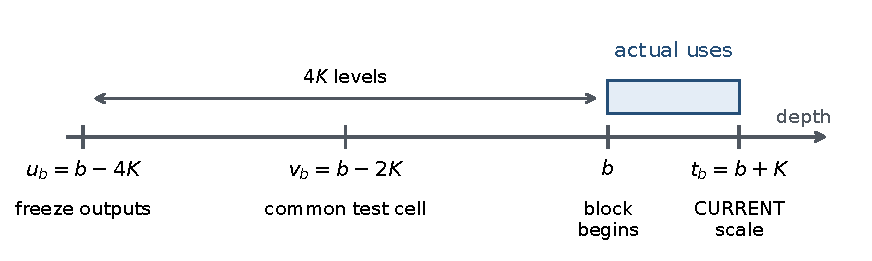
\includegraphics[width=.95\linewidth]{figures/depth-blocks.pdf}
 \caption{A block \([b,b+K)\) of dyadic depths.  Depth increases
 to the right and spatial scale decreases.  Coefficients are frozen
 at \(u_b=b-4K\).  The PRE and CURRENT graphs defined below are both
 evaluated on the same \(v_b=b-2K\) cell, using comparison scales
 \(r_{v_b}\) and \(r_{t_b}\), respectively, where \(t_b=b+K\).
 Each primary's first-match expansion is inherited unchanged across
 blocks.  The counting blocks in Figure~\ref{fig:counting-blocks}
 use a different partition.}
 \label{fig:depth-blocks}
\end{figure}

Fix a group \(G\), with primary center \(z\), and a basic-\(B\) role
\(l\).  A \emph{primary} in this discussion is an individual main
column \(\Phi\) available to the maximal pad of this role's outer ball
filter.  Distinct linear shifts of one vertex tag are distinct
primaries.  At its first match, on a cell \(I_0\), make one expansion
choice and retain that choice on every relevant descendant of \(I_0\).
The lists of primaries and their modes are therefore nested.  Separate
first-match branches may have separate expansions and private labels.
In particular, nothing in an already chosen mode list is resampled at
a later freezing time.

Choose an integer \(Q_0\), common to the roles of this group and within
the main budget, clearing the denominators of \(C_z\), and put
\(\vartheta=\theta_z/Q_0\).
For a uniformly random branch offset \(\rho\) on the unit cube, set
\[
 d^\rho(y)=\rho+\{\theta_z y-\rho\},\qquad
 p^\rho(y)=\lambda_z y^2+(\theta_z y)^T C_zd^\rho(y).
\]
The braces are coordinatewise fractional parts.  Choose a product
Gevrey cutoff \(\zeta^\rho\), periodic in \(\theta_z y-\rho\), with
\(0\le\zeta^\rho\le1\), vanishing within distance \(\delta_c\) of a
coordinate cut and equal to one outside distance \(2\delta_c\), where
\[
 \delta_c=\exp(-k^{C_c}).
\]
The exponent \(C_c\) is fixed sufficiently large after the main
budgets.  Translation invariance of the offset gives
\[
 \E_\rho\zeta^\rho(y)=c_\zeta\ge\tfrac12,\qquad
 \E_\rho|1-(\zeta^\rho(y))^2|^2
       \le C d_{\max}\delta_c
\]
at every \(y\).  A zero-dimensional horizontal parameter has the
constant convention \(\zeta^\rho=1\).
For each role and group the offset will be common to every branch and
time, and independent of the already completed main selections.

\begin{lemma}[First-match expansion and bounded lift]
\label{lem:first-match-lift}
At each first match \(I_0\), there is a finite, permanently labeled
expansion
\[
 \zeta^\rho(y)\varphi_\Phi(y)e(-c_l p^\rho(y))
 =\sum_m a_{\Phi,m}e(\lambda_m y^2+\gamma_m y)
       +O(\delta_c),\qquad y\in I_0,
\]
where all the modes belonging to this primary have the same
\(\lambda_m\).  We may use augmented mode atoms
\begin{equation*}
 \psi_m(y)=
 \left(
 \zeta^\rho(y)e(c_l p^\rho(y))
       e(\lambda_m y^2+\gamma_m y),
 \ \epsilon_{\mathrm m}^{1/2}\mathbf e_m
 \right).
 \tag{20}\label{eq:src-20}
\end{equation*}
Their private indices distinguish primaries and first-match
expansions.  For an admissible budget \(D_1\), with
\(\log D_1\le\operatorname{poly}(P,k)\), we have
\[
 |\lambda_m|\,|I_0|^2\le D_1,\qquad
 \sum_m|a_{\Phi,m}|\le D_1,
\]
and the number of modes is at most \(D_1\).  For two modes of this
primary,
\begin{equation*}
 \gamma_m-\gamma_{m'}=a\cdot(\theta_v,\vartheta),
 \qquad a\in\Q^{\dim(\theta_v,\vartheta)}
       \text{ has height at most }D_1 .
 \tag{21}\label{eq:src-21}
\end{equation*}
There is a block-independent pointwise linear operator
\(\mathscr R_{l,G}\), of uniformly bounded norm, mapping each frozen
outer ball output to exactly the corresponding synthesis of
Equation~\eqref{eq:src-20}.
\end{lemma}

\begin{proof}
The branch cutoff makes the conjugating factor a smooth quadratic
chart supported in a bounded branch cube.  At \(I_0\), the joint
difference data of \(v\) and \(z\) obey the endpoint version of
Equation~\eqref{eq:src-2}, with the harmless fixed factor \(c_l\).
Recenter at \(I_0\), choose one rational splitting there, and apply
Lemma~\ref{lem:chart-expansion}.  Its tail estimate gives the stated
uniform error and finite coefficient and count bounds.  A single
splitting gives a single effective quadratic coefficient for this
primary.  Recentring adds a common unrestricted linear shift; the
differences of the remaining linear shifts are rational combinations
of the two endpoint horizontal vectors.  Clearing \(Q_0\) gives
Equation~\eqref{eq:src-21}.  All these choices are made once.

Here is an explicit lift, which will also explain its operator
properties.  Write the main atom as
\(\Phi=(\varphi_\Phi,\epsilon_\Phi^{1/2}\mathbf e_\Phi)\), and set
\[
 q_\Phi(y)=
 \sum_m a_{\Phi,m}(\psi_m)_{\phys}(y)
       -(\zeta^\rho(y))^2\varphi_\Phi(y).
\]
It satisfies \(|q_\Phi|\le\delta_c\) on the matched subtree.
For a main augmented input \(F\), define the physical part of
\(\mathscr R_{l,G}F\) by
\[
 (\zeta^\rho)^2 F_{\phys}
 +\sum_{\Phi\ {\rm matched\ at}\ y}
       \frac{F_\Phi(y)}{\epsilon_\Phi^{1/2}}q_\Phi(y).
\]
Its mode coordinate \(m\), belonging to \(\Phi\), is
\[
 \epsilon_{\mathrm m}^{1/2}a_{\Phi,m}
       \frac{F_\Phi(y)}{\epsilon_\Phi^{1/2}},
\]
and is zero before the appropriate match.  The main count and inverse
weight bounds, followed by Cauchy--Schwarz, bound the physical
correction's pointwise operator norm by
\(\delta_c D_{\mathrm m}^{C}\).  Choose
\(\epsilon_{\mathrm m}>0\) so small that the squared norm of the
mode-coordinate map is bounded by one.  The preceding count and
coefficient estimates allow
\(\log(1/\epsilon_{\mathrm m})\le\operatorname{poly}(P,k)\).
Thus the whole lift has a uniform pointwise norm.

An outer ball output on a cell has a representation
\(\sum_\Phi\beta_\Phi\Phi\) with constant coefficients, including when
the projection is averaged.  Its main private coordinate is exactly
\(\epsilon_\Phi^{1/2}\beta_\Phi\).  Substitution in the displayed
definition gives
\(\sum_{\Phi,m}\beta_\Phi a_{\Phi,m}\psi_m\), as required.
The lift is pointwise and hence cell-local; it has not been commuted
through any projection.
\end{proof}

Put
\[
 \widetilde Z_{l,G,b}=\mathscr R_{l,G}Z_{l,G,u_b}
\]
on the retained branches.  It is a mode sum
\(\sum_m\alpha_m\psi_m\), with coefficients constant on the
\(u_b\)-cell.  Its available list may include every primary matched
for the maximal pad and rank, whether or not its coefficient is zero.
Fix a budget
\[
 D_*\ge e^k,\qquad \log D_*\le\operatorname{poly}(P,k),
\]
large enough for all the preceding mode counts, rational heights,
coefficient sums, inverse private weights, and \(Q_0\).
It also bounds the total number of available modes over all relevant
groups along a path, all actual cell/group uses, and the sums
\(\sum_m|\alpha_m|\) in normalized frozen evaluations.  These bounds
follow from the main coefficient bounds and
Lemma~\ref{lem:first-match-lift}; groups with a certified nonempty
endpoint already have historical data on that path.  We use disjoint
private coordinates to place all the required spaces in one Hilbert
space.

\subsection{The common progression multiplier and parameter order}

The common gauge has an additional property needed in the core
estimate.  Allow four different offsets \(\rho_j\), and let
\(y_j=y_0+jt\).  On the supports of their four cutoffs,
\(\prod_j e(c_jp^{\rho_j}(y_j))\) agrees with a smooth periodic
multiplier in
\((\vartheta y_{l'},\vartheta t)\), for any anchor \(l'\).  This
multiplier can be chosen bounded by one.

To verify this, write \(d_j=d^{\rho_j}(y_j)\).  Each
\(d_j-\theta_z y_j\) is an integer vector, so
\[
 k_j=d_j-(1-j)d_0-jd_1
\]
is an integer vector.  It is bounded, and locally constant away from
the branch cuts.  The identities
\(\sum_jc_j=\sum_jjc_j=\sum_jj^2c_j=0\) cancel the quadratic terms and
the terms containing \(d_0,d_1\), leaving
\[
 \prod_j e(c_jp^{\rho_j}(y_j))
   =e\!\left(\sum_jc_j(\theta_z y_j)^TC_zk_j\right).
\]
For each fixed carry choice the right side is an ordinary character
on the indicated torus, since \(Q_0\) clears \(C_z\).
Multiply it by slightly enlarged smooth cutoffs equal to one on the
required supports, and extend by zero at the cuts.  The pieces then
give the asserted smooth periodic function.  The same construction
works after changing the anchor, because the coordinate change has
integer coefficients.

Gevrey bounds for these cutoffs and the finitely many carry pieces
give admissible absolute Fourier coefficient sums, uniformly in the
offsets.  Enlarge \(D_*\) to cover those sums, including cutoff
products such as \((\zeta^\rho)^2\).  Only after this enlargement,
truncate their Fourier series with absolute tails at most
\(D_*^{-300}\).  Denote a common frequency cutoff by \(B_*\), where
\(\log B_*\le\operatorname{poly}(P,k)\).  Thus there is no circular
choice between a coefficient-sum budget and a Fourier truncation
radius.

We now fix the rest of the parameters.  Let \(\Delta=10\) and choose
a sufficiently small absolute \(\delta_*>0\).  Set
\[
 C_*=(10d_{\max}D_*)^{100d_{\max}^4},
 \qquad
 R_*^{\mathrm{ht}}=\lceil\log_2 C_*\rceil+2\Delta+10.
\]
Cramer's rule shows that expressing a height-\(D_*\) vector in a
basis of such vectors, in dimension at most \(d_{\max}\), uses
coefficients whose absolute values and common denominator are at
most \(C_*\).  Choose an integer \(J_*\) sufficiently large compared
with
\[
 \delta_*^{-2}d_{\max}R_*^{\mathrm{ht}}\log(2D_{\mathrm m}),
\]
and put
\[
 L_h=6^h,\qquad E_h=A_0^{h+1}\quad(0\le h\le J_*).
\]
Here \(A_0\) is an integer chosen as a sufficiently large fixed power
of \(C_*6^{R_*^{\mathrm{ht}}}B_*D_*\).
The notation \(E_h\) denotes a shift bound, not a projection.
Set \(\Xi=D_*^{1000}\).  Choose a rational height bound
\[
 \mathcal H>
 (d_{\max}C_*E_{J_*}B_*L_{J_*}Q_0\Xi)^{10},
\]
and then a gap factor
\[
 \mathcal T>(d_{\max}\mathcal H)^{C d_{\max}^4}\Xi
\]
with a sufficiently large absolute \(C\).
All their logarithms are polynomial in \(P,k\).

Finally choose the dyadic block length \(K\), still polynomial in
\(P,k\), sufficiently large after
\(\operatorname{poly}(d_{\max})(1+\log\mathcal H)+\log\mathcal T\).
In particular, if \(W\) is the width of a log packet in
Lemma~\ref{lem:height-bins} at height \(\mathcal H\), require
\(K\ge W+2\log_2\mathcal T\), after converting \(W\) to base-two
logarithms.  Increase \(K\) further whenever needed to make
\(D_*2^{-4K}\) smaller than any fixed inverse power of \(D_*\).
These choices have fixed polynomial degrees independent of \(q\).

For a mode let
\(\omega_m(x)=2\lambda_mx+\gamma_m\).
Its first match is no later than \(u_b\) if it is in the list frozen
at \(u_b\).  Lemma~\ref{lem:first-match-lift} therefore gives, on a
\(v_b\)-cell,
\[
 r_{v_b}\operatorname{osc}_{J}\omega_m
       \le C D_*2^{-4K}.
\]
This estimate also applies to every earlier retained mode when it is
viewed on a later pre-cell.

\subsection{Two component graphs}

On a retained \(v_b\)-cell \(J\), use the common list frozen at
\(u_b\).  At height \(h\), join two modes in the PRE graph if the
first bound below holds, and in the CURRENT graph if the second
holds, for some integral \(n\) with \(|n|_\infty\le E_h\):
\begin{equation*}
 \sup_{x\in J}
 \left|\omega_m(x)-\omega_{m'}(x)
                  +n\cdot\vartheta/L_h\right|
 \le \Xi/r_{v_b}
 \quad\hbox{or}\quad
 \le \Xi/r_{t_b},
 \quad\hbox{respectively}.
 \tag{22}\label{eq:src-22}
\end{equation*}
Write \(\mathcal E_h(m)\) and \(\mathcal F_h(m)\) for their
components.  PRE refines CURRENT.  Both graphs increase with \(h\):
an old witness is replaced by \(6n\), which is allowed since
\(A_0\ge6\).  They also increase along successive blocks on a path,
on retained lists, since the pre-cells shrink and the thresholds
increase.  For a set of modes \(\mathcal D\), let \(\pi(\mathcal D)\)
be its set of primary labels.  A \emph{minimal component} means the
component at height zero.

A primary with parameter vector \(\Theta=(\theta_v,\vartheta)\) is
\emph{nonexceptional} at this block if every rational vector \(a\)
of height at most \(\mathcal H\) satisfies
\begin{equation*}
 |a\cdot\Theta|\le\mathcal T^{-1}/r_{v_b}
 \qquad\hbox{or}\qquad
 |a\cdot\Theta|\ge\mathcal T/r_{t_b}.
 \tag{23}\label{eq:src-23}
\end{equation*}

\begin{lemma}[Exceptional blocks and the tiny rational space]
\label{lem:linear-exceptional}
Each primary is exceptional in at most \(C d_{\max}\) blocks on a
path.  At a nonexceptional block, let \(K_{\mathrm{rat}}\) be the
rational span of all height-\(\mathcal H\) vectors satisfying the
tiny alternative in Equation~\eqref{eq:src-23}.  If a vector of height
at most \(\mathcal H\) belongs to \(K_{\mathrm{rat}}\), then it too
satisfies that tiny alternative.
\end{lemma}

\begin{proof}
Fix the primary, put \(r_s=r_0 2^{-s}\), and write
\(\tau=\log_2\mathcal T\).  For a nonzero evaluation set
\(x(a)=\log_2(|a\cdot\Theta|r_0)\).
Exception at block start \(b\) means
\[
 b-2K-\tau<x(a)<b+K+\tau.
\]
Lemma~\ref{lem:height-bins} places all these \(x(a)\) in at most
\(d_{\max}\) packets of width \(W\).
A packet \([\alpha,\alpha+W]\) can cause an exception only when
\[
 \alpha-K-\tau<b<\alpha+W+2K+\tau.
\]
This interval has length at most \(4K\) by our choice of \(K\), so it
contains at most five starts of the \(K\)-spaced block schedule.
Zero evaluations are always tiny.

For the second assertion, choose a basis of tiny vectors from the
defining set.  Cramer's rule expresses any height-\(\mathcal H\)
vector in its span with coefficients of total absolute value at most
\((d_{\max}\mathcal H)^{C d_{\max}^3}\).
Its evaluation is consequently bounded by this factor times
\(\mathcal T^{-1}/r_{v_b}\).  The choice of \(\mathcal T\) makes this
strictly smaller than \(\mathcal T/r_{t_b}\).
The gap in Equation~\eqref{eq:src-23} then forces the tiny alternative.
\end{proof}

Put
\[
 K_B=\{w\in\Q^{\dim\theta_z}:(0,w)\in K_{\mathrm{rat}}\}.
\]
The space \(K_{\mathrm{rat}}\), and hence \(K_B\), can depend on the
primary and block.

\begin{lemma}[Height stabilization]
\label{lem:height-stabilization}
For a nonexceptional primary, all but
\(C d_{\max}R_*^{\mathrm{ht}}\) heights have the following property:
if two of its modes are in one CURRENT component at height \(h\),
then they are directly adjacent in the PRE graph at height
\(h-\Delta\).  We call these heights height-good for the primary.
\end{lemma}

\begin{proof}
Abbreviate \(R'=R_*^{\mathrm{ht}}\), and discard \(h<R'\).
If two modes of this primary are connected in CURRENT, sum the edge
witnesses along a simple connecting path.  There are at most \(D_*\)
edges.  Their quadratic parts cancel between the endpoints, because
the primary has one effective quadratic coefficient.  With \(a\)
from Equation~\eqref{eq:src-21}, this gives an integral \(m_h\) with
\(|m_h|_\infty\le D_*E_h\) and
\[
 |a\cdot\Theta+m_h\cdot\vartheta/L_h|
                   \le D_*\Xi/r_{t_b}.
\]
The vector \(a+(0,m_h/L_h)\) has height at most \(\mathcal H\).
Since \(D_*\Xi<\mathcal T\), the gap implies
\[
 a+(0,m_h/L_h)\in K_{\mathrm{rat}}.
\]

For each height \(i\), let \(V_i\) be the rational span of the
height-\(D_*\) vectors \(q'\) for which
\[
 q'+(0,m/L_i)\in K_{\mathrm{rat}}
 \quad\hbox{for some }m\in\Z^{\dim\theta_z},
 \qquad |m|_\infty\le D_*E_i.
\]
Let \(U_i\) be the rational span of the integer vectors in \(K_B\)
with size at most \(C_*^3D_*E_i\).
Both families increase.  Discard every \(h\) for which the rank of
either family changes between \(h-R'\) and \(h\).  There are at most
\(2d_{\max}R'\) such heights, since each rank can increase only
\(d_{\max}\) times.

At a remaining height, \(a\in V_h=V_{h-R'}\).  Express
\(a=\sum_jb_ja_j\) using a basis from the defining vectors at
\(h-R'\), with witnesses \(m_j\).  The \(b_j\) and their common
denominator are bounded by \(C_*\).  Subtracting the corresponding
relations in \(K_{\mathrm{rat}}\) shows that
\[
 m_h-6^{R'}\sum_jb_jm_j\in K_B.
\]
After clearing the common denominator this is an integer vector
whose size is at most \(C_*^3D_*E_h\); this follows directly from the
witness bounds and the choice of \(A_0\).
It belongs to \(U_h=U_{h-R'}\), which we denote by \(U\).

The lattice \(U\cap\Z^{\dim\theta_z}\) is saturated: if a nonzero
integer multiple of an integer vector belongs to \(U\), the vector
itself belongs to the rational space \(U\).
Thus the quotient
\(\Z^{\dim\theta_z}/(U\cap\Z^{\dim\theta_z})\) is free.  In an
integer basis of this quotient,
\[
 [m_h]=6^{R'}\sum_jb_j[m_j].
\]
The right side has integral coordinates.  The common denominator
bound and \(R'>\log_2C_*+2\Delta\) show, coordinate by coordinate,
that each is divisible by \(6^\Delta\): the valuations at both 2
and 3 are at least \(\Delta\).  Other denominator primes do not
affect these divisibilities.  Choose an integral lift \(m'\) of
\([m_h]/6^\Delta\).

Then \(m'-6^{R'-\Delta}\sum_jb_jm_j\in U\).
Choose linearly independent integer vectors of size at most
\(C_*^3D_*E_{h-R'}\) spanning the rational space \(U\), from the
definition of \(U_{h-R'}\).  Subtract integer multiples of these
vectors from \(m'\), rounding the coefficients of the preceding
difference.  The result remains an integer lift and satisfies
\[
 |m'|_\infty
 \le 6^{R'-\Delta}\sum_j|b_j|\,|m_j|_\infty
       +d_{\max}C_*^3D_*E_{h-R'}
 \le E_{h-\Delta}.
\]
The last inequality is one of the permitted fixed-power choices of
\(A_0\).  This rounding argument uses a small integer spanning set
of the rational space, not a lattice basis, and therefore incurs no
covolume factor.

Finally, \(m_h-6^\Delta m'\in U\subseteq K_B\), so
\[
 a+(0,m'/L_{h-\Delta})\in K_{\mathrm{rat}}.
\]
Its height remains at most \(\mathcal H\).
Lemma~\ref{lem:linear-exceptional} makes its evaluation at most
\(\mathcal T^{-1}/r_{v_b}\), which is below the PRE threshold.
Equation~\eqref{eq:src-21} gives the required direct edge.
\end{proof}

\subsection{Good modes and the bad-density count}

For \(h\ge\Delta\), call a mode \emph{good at \(h\)} when
\[
 \left\lfloor\log_{1.1}
       |\pi(\mathcal E_{h-\Delta}(m))|\right\rfloor
 =
 \left\lfloor\log_{1.1}
       |\pi(\mathcal F_h(m))|\right\rfloor
\]
and at least nine tenths of \(\pi(\mathcal F_h(m))\) are
nonexceptional and height-good at \(h\).
Every \(h<\Delta\) is bad.  A mode is a \emph{core mode} if at most
\(\delta_*(J_*+1)\) of its heights are bad; all other modes are
\emph{linear-side modes}.

\begin{lemma}[Coherence of good predicates]
\label{lem:good-predicates}
Good modes in one CURRENT component at height \(h\) have the same
PRE component at height \(h-\Delta\).  The core/side decision is
constant on each minimal PRE component.  Moreover, core modes in
one minimal CURRENT component have identical good predicates
throughout
\[
 \mathcal H_{\mathrm{up}}
   :=\{h\in\Z:\lceil4\delta_*J_*\rceil\le h\le J_*\},
\]
and have the same PRE components at height \(h-\Delta\) there.
Every core mode has bad proportion at most \(2\delta_*\) in
\(\mathcal H_{\mathrm{up}}\).
\end{lemma}

\begin{proof}
Write \(F=\pi(\mathcal F_h)\).  Each predecessor of a good mode has
more than \(|F|/1.1\) primaries.  Two such predecessor primary sets
intersect in more than
\((2/1.1-1)|F|\), and thus their intersection contains a
nonexceptional height-good primary, since fewer than one tenth of
the primaries are excluded.  The witnessing modes of that primary
belong to \(\mathcal F_h\).  Lemma~\ref{lem:height-stabilization}
joins them directly in PRE at \(h-\Delta\), so the two predecessor
components agree.

Modes in the same minimal PRE component have the same components
at every larger height and in CURRENT, so all their predicates
agree.  This proves the second assertion.
For the last assertion, two core modes have at most
\(2\delta_*(J_*+1)\) bad heights between them.
Our lower bound on \(J_*\) ensures that the interval of integer
heights below \(4\delta_*J_*\) contains more heights than this.
They therefore have a common good height \(h_0\) in that interval.
Their CURRENT components at \(h_0\) agree, since their minimal
CURRENT components agree.  The first assertion identifies their
PRE components at \(h_0-\Delta\).
Nesting then identifies all later PRE and CURRENT components, which
also identifies the corresponding predicates.
Finally, \(|\mathcal H_{\mathrm{up}}|\ge(1-4\delta_*)J_*\), so
the full-range bad count \(\delta_*(J_*+1)\) is at most
\(2\delta_*|\mathcal H_{\mathrm{up}}|\) for our small
\(\delta_*\) and sufficiently large \(J_*\).
\end{proof}

We give the counting argument for side modes explicitly.
The simple summation principle behind it will be used twice.

\begin{lemma}[Entry-rank summation]
\label{lem:entry-rank}
Let \(S_1\subseteq\cdots\subseteq S_T\) be nonempty finite sets with
\(|S_T|\le M\).  Suppose \(X_t\subseteq S_t\), and each element
belongs to at most \(A\) of the sets \(X_t\).  Then
\[
 \sum_{t=1}^T\frac{|X_t|}{|S_t|}
   \le A H_M,\qquad
 H_M=\sum_{r=1}^{\lfloor M\rfloor}\frac1r\le1+\log M.
\]
\end{lemma}

\begin{proof}
Enumerate elements by first entry into the increasing sets, breaking
ties arbitrarily.  A containing set for the element of entry rank
\(r\) has at least \(r\) elements.  Its total contribution is at most
\(A/r\).  Sum this bound over the elements.
\end{proof}

\begin{lemma}[Bad-density chains]
\label{lem:bad-density-chain}
Fix \(0<\delta,\beta<1\), integers \(J\ge\Delta\ge1\), and \(M\ge1\).
For \(1\le i\le N\), \(0\le h\le J\), let
\(\mathsf P_{i,h}\) and \(\mathsf C_{i,h}\) be nonempty sets of
primary labels, each increasing in \(h\), with cardinality at most
\(M\), and satisfying
\[
 \mathsf P_{i,h}\subseteq\mathsf C_{i,h}
       \subseteq\mathsf P_{i+1,h}\qquad(i<N).
\]
Let \(X_i\) be the exceptional primaries at position \(i\), each
primary exceptional at at most \(B\) positions.
For a fixed position, suppose each nonexceptional primary is
height-bad at at most \(A\) heights; write \(Y_{i,h}\) for these
height-bad primaries.
Declare \(h<\Delta\) bad, and for other heights declare \(h\) bad
if the floor logs of
\(|\mathsf P_{i,h-\Delta}|\) and \(|\mathsf C_{i,h}|\), to base
\(1.1\), differ, or if
\[
 \frac{|(X_i\cup Y_{i,h})\cap\mathsf C_{i,h}|}
      {|\mathsf C_{i,h}|}>\beta.
\]
Suppose each position has more than \(\delta(J+1)\) bad heights.
Set \(L=\lfloor\log_{1.1}M\rfloor\) and
\[
 Q=\Delta(L+1)+\beta^{-1}AH_M.
\]
If \(J+1\ge2Q/\delta\), then
\[
 N<\frac2\delta\bigl(L+\beta^{-1}BH_M\bigr).
\]
\end{lemma}

\begin{proof}
Write \(p_{i,h}\) and \(c_{i,h}\) for the two floor logs at height
\(h\).  Their values are integers between \(0\) and \(L\).
For \(h\ge\Delta\), the first failure indicator is bounded by
\[
 c_{i,h}-p_{i,h-\Delta}
 =(p_{i,h}-p_{i,h-\Delta})+(c_{i,h}-p_{i,h}).
\]
At fixed \(i\), the sum of the first term over \(h\) is at most
\(\Delta L\), because each increment of the increasing sequence
\(p_{i,h}\) is counted at most \(\Delta\) times.
At fixed \(h\), the temporal nesting gives
\[
 \sum_i(c_{i,h}-p_{i,h})
      \le c_{N,h}-p_{1,h}\le L.
\]
Including the initially bad heights, this contributes at most
\(N\Delta(L+1)+(J+1)L\) bad incidences.

The second failure indicator is bounded by \(\beta^{-1}\) times
the sum of the exceptional and height-bad fractions.
At fixed \(i\), Lemma~\ref{lem:entry-rank}, applied as \(h\)
increases, bounds the height-bad fractions by \(AH_M\).
At fixed \(h\), apply that lemma as \(i\) increases to bound the
exceptional fractions by \(BH_M\).
The total bad count is therefore at most
\[
 NQ+(J+1)(L+\beta^{-1}BH_M).
\]
On the other hand it is greater than \(\delta N(J+1)\).
The assumed lower bound for \(J+1\) absorbs \(NQ\) into half of
this last quantity, proving the result.
\end{proof}

\subsection{Separated projection rows}

We record the analytic consequence of graph nonadjacency that is
used both for side events and for tops.

\begin{lemma}[Separated mode rows]
\label{lem:separated-mode-rows}
Fix a role and group.  Consider a family of dyadic cells \(J_e\),
with a nonempty set \(\mathcal M_e\) of available mode labels on
each cell.  Suppose that along every path:
\begin{enumerate}
 \item the sets \(\mathcal M_e\) for cells containing that path are
 pairwise disjoint, and their total cardinality is at most \(D_*\);
 \item for distinct overlapping cells, every cross pair of mode
 atoms has normalized inner product on the smaller cell at most
 \(D_*^{-200}\) in absolute value.
\end{enumerate}
Assume the same cross-pair bound for distinct sets on the same cell.
Let \(P_e\) be orthogonal projection onto the restrictions of
\(\{\psi_m:m\in\mathcal M_e\}\), with output supported on \(J_e\).
Then
\[
 \sum_e\|P_eF\|^2\le C\|F\|^2
\]
with an absolute constant.

The cross-pair hypothesis holds if the sets have no shared or
adjacent modes in the later PRE graph and \(J_e\) are the associated
pre-cells.  It also holds for actual-use cells if the sets have no
shared or adjacent modes in the later CURRENT graph.
\end{lemma}

\begin{proof}
First verify the asserted oscillatory bound.  The common factor
\(e(c_lp^\rho)\) cancels between two physical atoms.
Fourier-expand \((\zeta^\rho)^2\) on the \(\vartheta\) torus,
retaining frequencies of size at most \(B_*\), with absolute
coefficient sum at most \(D_*\) and tail at most \(D_*^{-300}\).
At height zero these shifts are allowed because \(E_0=A_0\)
exceeds \(B_*\).  At a larger height the corresponding shifts are
multiplied by \(L_h\), and
\(B_*L_h\le E_h\), by the choice of \(A_0\).

For each retained shift, nonadjacency gives a point of the relevant
pre-cell where the absolute phase derivative exceeds its graph
threshold.  The affine-slope oscillation bound makes the absolute
derivative at every point of that cell at least half the threshold.
The derivative is affine and of constant sign, so the elementary
first-derivative oscillatory estimate on any interval applies.
For PRE on a pre-cell it bounds the normalized integral by
\(C/\Xi\).  For CURRENT on an actual cell \(I\), it gives the same
bound, since \(|I|\ge r_{t_b}\).
The cutoff coefficient sum and tail give
\[
 C D_*/\Xi+D_*^{-300}\le D_*^{-200}
\]
after increasing the starting budget.  Distinct labels have
orthogonal private coordinates, so they contribute no other inner
product.  Earlier modes satisfy the same slope-variation estimate
on the later pre-cell by inheritance.

For the Bessel conclusion it suffices, by duality, to bound the
synthesis of arbitrary \(f_e\) in these projection ranges.
Write \(f_e=\1_{J_e}\sum_{m\in\mathcal M_e}\beta_{e,m}\psi_m\), and
put \(b_e=(\sum_m|\beta_{e,m}|^2)^{1/2}\).
Private coordinates give
\[
 |J_e|b_e^2\le D_*^2\|f_e\|^2.
\]
For an overlapping pair, constancy of these coefficients on their
cells and the cross-pair estimate bound its inner product by
\[
 D_*^{-199}|J_e\cap J_f|\,b_eb_f.
\]
There are at most \(D_*\) participating rows at a path point.
Consequently
\[
 \begin{split}
 \sum_{e\ne f}|\langle f_e,f_f\rangle|
 &\le D_*^{-199}
       \int_R\left(\sum_{e:x\in J_e}b_e\right)^2\,dx\\
 &\le D_*^{-198}\sum_e|J_e|b_e^2
 \le D_*^{-196}\sum_e\|f_e\|^2 .
 \end{split}
\]
Adding the diagonal proves the synthesis bound and hence the row
Bessel bound.  This calculation uses a pathwise label count; it
does not count the number of unused depths between rows.
\end{proof}

\begin{lemma}[Composition with the lift and main histories]
\label{lem:lifted-row-compression}
Fix a role.  For each group, suppose a family of mode projection
rows \(P_e\), supported on cells \(J_e\), has squared Bessel bound
at most \(G_0\).  Suppose \(J_e\subseteq u_e\), where \(u_e\) is a
usable main endpoint cell with a downstream actual-use certificate.
The mode list of \(P_e\) is drawn from the list available at \(u_e\).
Then the frozen row outputs
\[
 P_e\,\mathscr R_{l,G}\,
       \overline L_{l,G,u_e}\,\mathcal B_{l,u_e}B_{l,u_e}
\]
satisfy a joint squared bound \(G_0|R|\), over all groups and rows.
Here \(B_{l,u_e}\) is the basic-\(B\) input generated by its specified
constituent main projection families from the original normalized input.
\end{lemma}

\begin{proof}
Initially omit the shared histories.  For one group,
\(P_e\mathscr R_{l,G}\) is a Bessel family with the same type of
bound, since \(\mathscr R_{l,G}\) is one fixed bounded operator.
It depends only on \(J_e\), and therefore also only on the
containing decision cell \(u_e\).  Lemma~\ref{lem:compression}
applies to the outer individual main ball projection at that cell.
It permits arbitrarily many rows with the same decision cell.
Its loss is a fixed power of \(\log(2D_{\mathrm m})\).
Averaging the pad choices uses the triangle inequality in the
Hilbert sum of row outputs and costs no number-of-pads factor.

Let \(A_G\) be the resulting row operator for this group.
For an individual outer projection its row adjoint has the order
\[
 L_{l,G,u_e}\,\mathscr R_{l,G}^*P_e.
\]
Its range is thus in the main ball range on the entire cell
\(u_e\).  With an averaged projection, it lies in the sum of these
usable ranges.  Lemma~\ref{lem:usable-bessel} gives
\[
 \left\|\sum_G A_G^*w_G\right\|^2
       \le C\sum_G\|A_G^*w_G\|^2
       \le G_0\sum_G\|w_G\|^2.
\]
Duality proves the joint Bessel bound before the shared histories.
This is the step for which full endpoint cells and their downstream
certificates are needed.

Finally apply Lemma~\ref{lem:compression} again to these joint rows,
with decision cells \(u_e\), to insert the shared histories.
Expand complements and the fixed signed sum in \(B_l\), and keep
the positive averages as averages.  Their product lengths are
\(O(\log\mathcal L)\), their column log-budgets are polynomial in
\(k\), and the number of signed terms is a small overhead.
The compression loss is therefore \(G_0\).
The original input has squared norm at most \(|R|\).
All operators have remained in their indicated order.
\end{proof}

\begin{proposition}[Square energy of the linear side]
\label{prop:linear-side}
For each basic-\(B\) role, on every retained \(v_b\)-cell let
\(V_{l,G,b}\) be the exact subtotal of the linear-side modes in
\(\widetilde Z_{l,G,b}\), including their private coordinates.
Set it to zero on branches without a needed output or certificate.
Then
\[
 \sum_{G,b}\|V_{l,G,b}\|^2\le G_0|R|.
\]
In particular these functions satisfy Equation~\eqref{eq:src-17},
uniformly in the branch offsets.
\end{proposition}

\begin{proof}
Fix \(l,G\).  An event is a triple \((b,J,\mathcal E)\), where
\(J\) is a retained \(v_b\)-cell and \(\mathcal E\) is a minimal
PRE component of side modes.  Such a component consists entirely
of side modes by Lemma~\ref{lem:good-predicates}.
Split block indices into their ten congruence classes.
Within one class, link an event to a later event on a descendant
path when some of their modes agree or are adjacent in the later
minimal PRE graph.

For two linked events, every earlier CURRENT edge persists in the
later PRE graph.  Indeed the later pre-cell is contained in the
earlier pre-cell, the mode lists persist, and the separation of
block starts gives \(v_{\rm later}\ge t_{\rm earlier}\).
The minimal PRE link also persists at every height.
Consequently, choosing any mode in each event of a linked chain
gives
\[
 \pi(\mathcal E^{(i)}_h)
 \subseteq\pi(\mathcal F^{(i)}_h)
 \subseteq\pi(\mathcal E^{(i+1)}_h)
\]
at every height.

Apply Lemma~\ref{lem:bad-density-chain} with
\[
 M=D_{\mathrm m},\quad \beta=\tfrac1{10},\quad
 A=C d_{\max}R_*^{\mathrm{ht}},\quad B=C d_{\max},
 \quad\delta=\delta_*.
\]
The height multiplicity comes from
Lemma~\ref{lem:height-stabilization}; the exceptional-block
multiplicity comes from Lemma~\ref{lem:linear-exceptional}.
Every event mode has more than \(\delta_*(J_*+1)\) bad heights.
Our choice of \(J_*\) meets the lemma's lower bound.  Thus every
chain has length at most
\[
 C_{\delta_*}d_{\max}\log(2D_{\mathrm m}).
\]
For clarity, the inequality being absorbed is
\[
 \delta_*N(J_*+1)
 \lesssim N d_{\max}R_*^{\mathrm{ht}}\log(2D_{\mathrm m})
       +(J_*+1)d_{\max}\log(2D_{\mathrm m}).
\]
Although \(R_*^{\mathrm{ht}}\) depends on the mode budget, it
disappears from the final chain-length bound.

Give each event its longest-chain level.  Linked events have
different levels.  Distinct overlapping events in one level
therefore have no shared or adjacent modes in the later minimal
PRE graph.  Events on one cell are distinct components and have
the same separation.  Their label sets are pairwise disjoint on
a path, with total count at most \(D_*\).
Lemma~\ref{lem:separated-mode-rows} applies to the orthogonal
projection \(P_{\mathcal E,J}\) onto the augmented columns of
\(\mathcal E\), restricted to \(J\).
Summing the ten congruence classes and the bounded number of levels
gives squared Bessel bound \(G_0\) for the event rows.

The decision cell for a row is its containing \(u_b\)-cell.
Apply Lemma~\ref{lem:lifted-row-compression} to obtain
\begin{equation*}
 \sum_{G,b,J,\mathcal E}
   \|P_{\mathcal E,J}\widetilde Z_{l,G,b}\|^2
       \le G_0|R|.
 \tag{24}\label{eq:src-24}
\end{equation*}
Zero outputs from pre-depths before the attempt were omitted.

It remains to pass from projections to exact coefficient
subtotals.  Write \(T_{\mathcal E,J}\) for that subtotal.
Every mode outside \(\mathcal E\) is PRE-nonadjacent to every mode
inside it.  The oscillatory estimate in
Lemma~\ref{lem:separated-mode-rows}, the private-coordinate lower
bound, and \(\sum_m|\alpha_m|\le D_*\) give
\[
 \|P_{\mathcal E,J}\widetilde Z_{l,G,b}
                         -T_{\mathcal E,J}\|_{2,J}
       \le D_*^{-190}.
\]
For example, pairing the complementary subtotal against a unit
vector in this range costs its coefficient \(\ell^1\) norm,
at most \(D_*^{3/2}\), times the outside coefficient sum and the
pair bound \(D_*^{-200}\).
Within one event level the number of occurrences on a path is at
most \(D_*\).  The number of levels is \(G_0\), and the budgets
also include all groups present on these full-cell paths.
Thus the squared additive errors summed over all events are
negligible compared with \(|R|\).

Finally, on each \(J\) the different minimal PRE subtotals are
almost orthogonal by the same coefficient calculation.  Their sum
is \(V_{l,G,b}\).  Summing their squared norms in
Equation~\eqref{eq:src-24} therefore proves the assertion.
\end{proof}

\subsection{Fixing offsets and separating the side terms}

Define \(A_{l,G,b}\) as the exact core subtotal of
\(\widetilde Z_{l,G,b}\).  In a basic-\(B\) role put
\[
 S_{l,G,s}=Z_{l,G,s}-Z_{l,G,u_b}+V_{l,G,b},
 \qquad b\le s<b+K.
\]
In a basic-\(U\) role set \(S_{l,G,s}=Z_{l,G,s}\), with no core
term.  Taking physical components gives
\[
 Z_{l,G,s}=A_{l,G,b}+S_{l,G,s}+\mathcal E_{l,G,b},
 \qquad
 \mathcal E_{l,G,b}
       =(Z_{l,G,u_b})_{\phys}
           -(\widetilde Z_{l,G,b})_{\phys}.
\]
Only this displayed identity uses the scalar error
\(\mathcal E_{l,G,b}\); the mode subtotals themselves retain their
augmented coordinates.

We can choose the offsets so that the errors have negligible
integrated square energy on all actual uses.  To see this without
any independence assumption about the eventual core choices, let
\[
 Z_{l,G,u_b}=\sum_\Phi\beta_\Phi\Phi.
\]
The explicit lift gives
\[
 \mathcal E_{l,G,b}
 =(1-(\zeta^\rho)^2)(Z_{l,G,u_b})_{\phys}
                   -\sum_\Phi\beta_\Phi q_\Phi.
\]
The coefficients \(\beta_\Phi\), their normalized main bounds, and
the full collection of actual main uses were fixed before drawing
the offsets.  On its own \(u_b\)-cell, an outer main projection has
coefficient sum and physical supremum at most \(D_{\mathrm m}^C\).
This bound follows from its private weights and the normalized
input on that cell and does not lose a factor from the lag \(4K\).
Therefore
\[
 \E_\rho|\mathcal E_{l,G,b}(y)|^2
       \le D_{\mathrm m}^C d_{\max}\delta_c
\]
on every needed branch.  Summing over all original actual
cell/group uses, before any offset-dependent mode selection or
pruning, gives
\[
 \E_\rho
 \sum_{l,G,I\ {\rm used}}|I|\,
      \|\mathcal E_{l,G,b(I)}\|_{2,I}^2
       \le D_{\mathrm m}^C d_{\max}\delta_c\,|R|.
\]
By enlarging \(C_c\), this is smaller than any required fixed
inverse main-budget power times \(|R|\).
Choose offsets satisfying the resulting bound and keep them fixed.
Subsequent core decisions, restrictions, and stopping only remove
nonnegative terms from this error sum.  They need not be independent
of the offsets.  Proposition~\ref{prop:linear-side} was uniform in
the offsets, so its estimate remains valid for this choice.

The rolling variation bounds and the path pruning in
Section~\ref{sec:sides}, now supplied with
Proposition~\ref{prop:linear-side}, give
\[
 \sum_{s,G}\|S_{l,G,s}\|_{2,I_s}^2\le P^C
\]
along a retained path.  Individual core sizes are also at most
\(P^C\): use the bounded lift,
\(Z_{u_b}=Z_s-(Z_s-Z_{u_b})\), and the corresponding bounds for
\(V_{l,G,b}\).  The local absolute \(L^2\) form bound and
Cauchy--Schwarz over the original actual uses now make every term
containing a physical error negligible; its other three sizes are
at most \(P^C\), and the original path multiplicity is within the
main budget.

Expand Equation~\eqref{eq:src-14} with these arguments.  Keep the
terms with at least three core roles for the next section.
For a term with exactly two side roles, replace its two core
complements by the whole current \(Z_{G,s}\) arguments.
The corrections have at least three sides, apart from the physical
errors just treated.  Proposition~\ref{prop:side-estimate} applies
to the resulting two-side terms with whole complements, through
Lemma~\ref{lem:transfer}; it also bounds the terms with three or
four sides.  Its powered costs use the minimum in
Equation~\eqref{eq:src-11} and obtain the factor
\(\eta^\varepsilon\) for any fixed sufficiently small
\(\varepsilon>0\).
An original basic-\(U\) role has remained a mandatory side throughout.
In particular, the restored complementary arguments are the
specified basic-\(B\) inputs required by the pair-smallness estimate.

\subsection{Hereditary representatives}

Fix a height \(h\in\mathcal H_{\mathrm{up}}\) and a basic-\(B\)
role.  Call a CURRENT component \(\mathcal F_h\)
\emph{successful} if it contains a core mode good at this height.
By Lemma~\ref{lem:good-predicates}, all its good modes have one
predecessor \(\mathcal E_{h-\Delta}\).  Its \emph{type} is the pair
\[
 \left(
  \left\lfloor\log_{1.1}|\pi(\mathcal E_{h-\Delta})|\right\rfloor,
  \left\lfloor\log_{1.1}|\mathcal E_{h-\Delta}|\right\rfloor
 \right).
\]
The first coordinate counts primaries and the second counts modes.
Both are needed in the following construction.

\begin{lemma}[Hereditary representatives]
\label{lem:hereditary-labels}
Fix the height, role, group, and type.  We can choose a representative
mode \(a\in\mathcal E_{h-\Delta}\) for every successful component so
that it is inherited whenever an earlier successful predecessor on
the same path is contained in the current predecessor.
Distinct representatives on comparable actual-use cells have no
adjacent pair of component modes in the later CURRENT graph.
In particular, if \(I,I'\) are such cells and \(x_*\in I\cap I'\),
then their distinct representatives satisfy
\begin{equation*}
 \left|\omega_a(x_*)-\omega_{a'}(x_*)
                     +n\cdot\vartheta/L_h\right|
  >\frac{\Xi}{2}
       \max\bigl(|I|^{-1},|I'|^{-1}\bigr),
 \qquad n\in\Z^{\dim\theta_z},\quad |n|_\infty\le E_h .
 \tag{25}\label{eq:src-25}
\end{equation*}
\end{lemma}

\begin{proof}
Say an earlier successful component links to a later one if a mode
of the earlier component is equal or CURRENT-adjacent, at the later
height-\(h\) graph, to a mode of the later component.
Persistence of the earlier CURRENT edges then gives
\(\mathcal F_{\rm early}\subseteq\mathcal F_{\rm late}\).
Write \(F=\pi(\mathcal F_{\rm late})\).
Later goodness and the common first type coordinate imply
\[
 |\pi(\mathcal E_{\rm late})|>|F|/1.1,\qquad
 |\pi(\mathcal E_{\rm early})|
    >|\pi(\mathcal E_{\rm late})|/1.1
    >|F|/1.1^2 .
\]
Both predecessor primary sets lie in \(F\).
Their intersection therefore has more than
\((1/1.1+1/1.1^2-1)|F|\) elements, a proportion greater than
one tenth.  It contains a later nonexceptional height-good primary.
Two witnessing modes of that primary lie in
\(\mathcal F_{\rm late}\), one from each predecessor.
Lemma~\ref{lem:height-stabilization} joins them in the later PRE
graph at \(h-\Delta\).  Earlier PRE edges persist, so
\[
 \mathcal E_{\rm early}\subseteq\mathcal E_{\rm late}.
\]
The same argument at one block reduces to uniqueness of the good
predecessor.

Now process the considered pre-cells in block order.  If a current
predecessor contains an earlier successful predecessor of this
type on its path, inherit its representative.  Otherwise choose
any mode of the current predecessor by a fixed ordering of labels.
To prove consistency, take any two earlier predecessors contained
in the current one.  Equality of the second type coordinate gives
each more than \(1/1.1\), and in particular more than one half, of
the current mode count.  They intersect.  They lie on one path,
so their shared mode is a link from the earlier to the later of
them.  The inclusion just proved makes them nested.
By induction all their inherited representatives agree.
Comparable pre-cell data occur on ancestors, and the list and
graph are constant throughout each pre-cell, so this defines
representatives consistently for all its actual descendants.

If two components on comparable uses with this type had equal or
adjacent modes in the later CURRENT graph, the same inclusion
argument would force inheritance of the earlier representative.
Thus distinct representatives imply the asserted nonadjacency
of every cross pair of modes.
Suppose \(I'\) is the later, smaller actual cell, in a block with
pre-cell \(J'\) and comparison depth \(t_{b'}\).
For each allowed \(n\), nonadjacency gives
\[
 \sup_{x\in J'}
   |\omega_a(x)-\omega_{a'}(x)+n\cdot\vartheta/L_h|
       >\Xi/r_{t_{b'}}.
\]
The slope oscillation on \(J'\) is negligible compared with this
threshold, so its value at \(x_*\) is greater than
\(\Xi/(2r_{t_{b'}})\).
Since \(|I'|\ge r_{t_{b'}}\), this implies
Equation~\eqref{eq:src-25}.
\end{proof}

The representatives are mode labels, not numerical frequencies;
different labels may initially have identical scalar atoms.
Equation~\eqref{eq:src-25} is the separation obtained for the
distinct labels that actually occur with one fixed type on a path.
All lattice shifts in this equation, and in the later frequency
boxes, are integral.

\subsection{Sizes of components}

At an actual cell \(I\) in the block, for each successful
\(\mathcal F=\mathcal F_h\) define
\begin{equation*}
 \sigma_{\mathcal F}^2
   =\sum_{\mathcal D\subseteq\mathcal F}
      \left(
        \|A_{\mathcal D}\|_{2,I}
        +D_*^{-30}
          \sum_{\substack{m\ {\rm core}\\m\in\mathcal D}}
                         |\alpha_m|
      \right)^2 .
 \tag{26}\label{eq:src-26}
\end{equation*}
Here \(\mathcal D\) ranges over the minimal CURRENT components, and
\(A_{\mathcal D}\) is its full core subtotal, in the augmented mode
space.  The small coefficient term will absorb later uniform
linearization and Fourier-truncation errors without replacing
the component's \(L^2\) amplitude by its coefficient sum.

Let \(P_{\mathcal F,I}\) denote orthogonal projection on the
restrictions to \(I\) of all mode labels in \(\mathcal F\), and let
\(V_{\mathcal F}\) be the exact linear-side subtotal on those labels.

\begin{lemma}[Component-size comparison]
\label{lem:component-size}
At every actual cell,
\begin{equation*}
 \begin{split}
 \sigma_{\mathcal F}^2
 &\lesssim
    \|P_{\mathcal F,I}\widetilde Z_{l,G,b}\|_{2,I}^2
       +\|V_{\mathcal F}\|_{2,I}^2+D_*^{-50},\\
 \sum_{\mathcal F}\|V_{\mathcal F}\|_{2,I}^2
 &\lesssim\|V_{l,G,b}\|_{2,I}^2 ,
 \end{split}
 \tag{27}\label{eq:src-27}
\end{equation*}
where the second sum can be over the successful components.
The same almost orthogonality controls arbitrary coefficient
subtotals separated into distinct minimal CURRENT components.
\end{lemma}

\begin{proof}
Modes in different minimal CURRENT components are nonadjacent in
that graph.  The oscillatory proof of
Lemma~\ref{lem:separated-mode-rows} applies on \(I\), because
\(|I|\ge r_{t_b}\).  Its synthesis calculation on this single
cell shows that for arbitrary subtotals \(f_{\mathcal D}\) in
distinct components,
\[
 \left\|\sum_{\mathcal D}f_{\mathcal D}\right\|_{2,I}^2
   \asymp\sum_{\mathcal D}\|f_{\mathcal D}\|_{2,I}^2 .
\]
The constants are uniform, since the off-diagonal norm is at most
a fixed small inverse power of \(D_*\) after the private-coordinate
bound.  In particular this is a two-sided estimate and applies
to any subset of labels inside each component.

Let \(T_{\mathcal F}\) be the full coefficient subtotal on
\(\mathcal F\).  Its core subtotal is
\(A_{\mathcal F}=T_{\mathcal F}-V_{\mathcal F}\).
The preceding estimate bounds the sum of the squared core
component norms in Equation~\eqref{eq:src-26} by
\(C\|A_{\mathcal F}\|_{2,I}^2\).
The contribution of the coefficient floors is at most
\[
 C D_*^{-60}\left(\sum_m|\alpha_m|\right)^2
       \le C D_*^{-58}.
\]
Every mode outside \(\mathcal F\) is CURRENT-nonadjacent to the
modes inside.  Pairing against a unit vector of its augmented span,
as in the proof of Proposition~\ref{prop:linear-side}, gives
\[
 \|P_{\mathcal F,I}\widetilde Z_{l,G,b}
                    -T_{\mathcal F}\|_{2,I}\le D_*^{-190}.
\]
Combine these observations with
\(\|T_{\mathcal F}-V_{\mathcal F}\|^2
\le2\|T_{\mathcal F}\|^2+2\|V_{\mathcal F}\|^2\)
to obtain the first bound, with its stated generous error.

Finally decompose \(V_{l,G,b}\) by all CURRENT components at
height \(h\), whether successful or not.  They too are separated,
so the two-sided almost orthogonality gives the second bound after
discarding the nonsuccessful terms.
\end{proof}

\subsection{First tops and the pathwise label bound}

\begin{proposition}[Top count]
\label{prop:top-count}
After removing summands on first stopping cells of arbitrarily
small fixed total relative length, the following holds on every
retained path.  Fix a core role \(j\), a height
\(h\in\mathcal H_{\mathrm{up}}\), a type, and a dyadic amplitude bin
\(\sigma_j\le\sigma_{\mathcal F}<2\sigma_j\).
Let \(\mathcal A_j^G\) be the distinct representatives of
successful components of this type actually used in that bin
along the path.  Then
\begin{equation*}
 \sum_G|\mathcal A_j^G|
      \le \min(D_*,P^C\sigma_j^{-2}).
 \tag{28}\label{eq:src-28}
\end{equation*}
The exponent \(C\) is fixed.  Enlarging \(D_*\) by a fixed power is
harmless in this statement.  On retained uses, all component sizes
and full local side sizes are at most \(P^C\), and for a side role
\[
 \sum_{s,G}\|S_{l,G,s}\|_{2,I_s}^2\le P^C.
\]
\end{proposition}

\begin{proof}
First fix one height, type, and dyadic threshold
\(D_*^{-1}\le\sigma\le D_*^2\).
For each group and representative, take the first actual-use
cells on each spatial branch for which
\(\sigma_{\mathcal F}\ge\sigma\).  Call them its first tops.
First tops of the same representative do not overlap.
For two overlapping first tops of different representatives,
Lemma~\ref{lem:hereditary-labels} gives CURRENT nonadjacency of
all their component modes at the later block.
The label sets are therefore disjoint on a path, with total
mode count at most \(D_*\).
Lemma~\ref{lem:separated-mode-rows} proves a uniform Bessel bound
for the rows \(P_{\mathcal F,I}\) at these tops.

The row is supported on its actual cell \(I\), which is contained
in the \(u_b\)-cell of its frozen list.  This remains a valid
decision cell for Lemma~\ref{lem:lifted-row-compression}, even if
many rows share it.  All these endpoint cells have the top itself
as a downstream actual-use certificate.  That lemma gives
\[
 \sum_{\rm tops}
      \|P_{\mathcal F,I}\widetilde Z_{l,G,b}\|^2
          \le G_0|R|.
\]
No restriction of the input ball projection to the smaller top
cell is made in this step.

For the side contributions in Equation~\eqref{eq:src-27}, sum
first at one depth of one block.  The actual cells there are
disjoint; at each cell the component sum is bounded by
\(\|V_{l,G,b}\|_{2,I}^2\).  Summing the at most \(K\) depths and
then applying Proposition~\ref{prop:linear-side} gives
\[
 \sum_{\rm tops}|I|\,\|V_{\mathcal F}\|_{2,I}^2
       \le C K\sum_{G,b}\|V_{l,G,b}\|^2
       \le K G_0|R|.
\]
Since \(\sigma_{\mathcal F}\ge\sigma\), the size comparison now
yields
\[
 \sigma^2\sum_{\rm tops}|I|
       \le C(1+K)G_0|R|
              +C D_*^{-50}\sum_{\rm tops}|I|.
\]
The final term can be absorbed, because
\(\sigma^2\ge D_*^{-2}\).  Thus
\[
 \sigma^2\sum_{\rm tops}|I|
                 \le C(1+K)G_0|R|.
\]

There are only polynomially many choices in \(P,k\) of height,
type, and threshold: the counts are controlled by \(J_*\) and
powers of \(\log(2D_*)\).
For each choice let
\(N_\sigma(x)=\sum_{\rm tops}\1_I(x)\), summing also over groups.
The displayed integral bound and Markov's inequality give a
pathwise bound
\(N_\sigma(x)\le P^C\sigma^{-2}\) outside a set of as small a
fixed measure as desired, after enlarging \(C\) and the constant
in the stopping threshold.  Summing these exceptional measures
over all the choices still costs a small fraction of \(|R|\).
Implement the cut by stopping at the first actual cells where
the corresponding partial top count exceeds its threshold.
All the estimates are valid again on normalized subroots, so
these summands are assigned to fresh attempts.

If a representative is used in the bin
\([\sigma_j,2\sigma_j)\) on a retained path, its first
\(\sigma_j\)-top is an ancestor of that use.
It too is retained; otherwise the descendant summand would
already have been sent to a fresh attempt.
Different representatives have different such tops on the path,
so their count is at most \(N_{\sigma_j}(x)\).
The full mode-label budget gives the additional bound \(D_*\).
For \(\sigma_j<D_*^{-1}\), that full bound alone implies the
minimum in Equation~\eqref{eq:src-28}.
Above the tested threshold range the bins are empty by the
coefficient and atom bounds, after the allowed budget enlargement.

The side square bound is the pruning already made following
Proposition~\ref{prop:linear-side}.
For amplitude control, \(Z_{u_b}=Z_s-(Z_s-Z_{u_b})\), the bounded
pointwise lift, and the side bounds give
\(\|\widetilde Z_{l,G,b}\|_{2,I}
 +\|V_{l,G,b}\|_{2,I}\le P^C\).
Projection is a contraction on \(I\), so
Lemma~\ref{lem:component-size} bounds
\(\sigma_{\mathcal F}\) by \(P^C\) as well.
\end{proof}

The statements of Lemmas~\ref{lem:good-predicates}
and~\ref{lem:hereditary-labels}, the size definition
Equation~\eqref{eq:src-26}, and Proposition~\ref{prop:top-count}
are the inputs to the core estimate.  In particular,
upper-range good-height masks select unions of full core
subtotals in minimal CURRENT components, and the representatives
used by a fixed role, height, type, and amplitude bin satisfy both
the separation in Equation~\eqref{eq:src-25} and the joint
group count in Equation~\eqref{eq:src-28}.

\section{Successful heights and concentration across scales}
\label{sec:counting}

We estimate the terms containing at least three core arguments.  Throughout
this section we work on one retained attempt with root $R$, and on one of
the search leaves in the localization.  All the conclusions are uniform
in that leaf.  We use the mode construction, the retained path bounds, and
the notation of Section~\ref{sec:linearization}.  In particular,
$\log D_*\leq\operatorname{poly}(P,k)$, whereas every loss described below
as $P^C$ has an absolute exponent.  The exponent can be increased a finite
number of times without changing this convention.

We first sum the common-height histories and reduce each fixed
configuration to frequency tests with torus amplitude bounds.
A finite sparse-count lemma then controls the tested tuples across
scales.  Finally, interpolation sums the group, amplitude, and
frequency parameters.  The original cell minimum is applied before
subadditivity, keeping each tuple count inside its power; numerical
errors are estimated separately in absolute value.

\subsection{A common successful height}

Fix a term with $m_0\in\{3,4\}$ core roles.  If $m_0=3$, denote the
remaining, side role by $l$.  Fix an actual use $I=I_s$, a group $G$, and
a point $x_*\in I$.  Write $r=|I|$ and $R_s=r^{-1}$.  The choice of $x_*$
is arbitrary; eventually we integrate the resulting estimates over such
points.  All mode lists here are finite.

Sample heights independently and uniformly from the upper height range.
For a fixed tuple of core modes, retain the first sampled height at which
all its roles are good.  A core mode has bad density at most $2\delta_*$
in this range, so the probability of success in one trial is at least
$1-2m_0\delta_*>0$.  Consequently the first-success rule gives an exact
identity in expectation for each pure tuple, and hence for the finite
mode expansion of the form.

Suppose that success occurs at trial $n+1$, with final height $h$.
Assign each of the previous $n$ failed trials to its first failing role,
in the natural order of the roles.  There are at most $m_0^n$ assignments.
For a fixed assignment the conditions in each role form a product mask
on its modes: that role must fail at the trials assigned to it, and must
succeed at the earlier roles' required positions.  Group the selected
modes at the final CURRENT components $\mathcal F_j$.  The coherence of
the upper-height predicates on a minimal CURRENT component implies that
the selected modes are unions of entire core subtotals
$A_{\mathcal D}$ from \eqref{eq:src-26}.  Final success puts all of them
in the unique good predecessor of $\mathcal F_j$.  Let $a_j$ denote the
inherited representative of that predecessor.

Put
\[
 \xi=\frac{\vartheta}{L_{h-\Delta}},\qquad
 \gamma_j^*=\omega_{a_j}(x_*).
\]
A PRE path from a selected mode to its representative gives an integral
vector $n_j$ with $|n_j|_\infty\leq D_*E_{h-\Delta}$ such that its
instantaneous slope at $x_*$ differs from
$\gamma_j^*+n_j\cdot\xi$ by at most $D_*\Xi/r_{v_b}$.
The pre-lag makes the product of this error with $r$ arbitrarily small
at a prescribed inverse power of $D_*$.  The quadratic Taylor error is
equally small: the mode was admitted by $u_b$, and its curvature at its
admission scale was bounded by $D_*$.  The phase constant at $x_*$ can
be absorbed into its coefficient.  Thus the physical selected argument,
up to a uniform error bounded by $D_*^{-150}$ times its absolute
coefficient sum, has the form
\begin{equation*}
 e\big(c_jp^{\rho_j}(y_j)\big)
 e\big(\gamma_j^*(y_j-x_*)\big)
 g_j\big(\xi(y_j-x_*)\big).
 \tag{29}\label{eq:src-29}
\end{equation*}
Here $g_j$ is the true periodic cutoff times a finite trigonometric
polynomial.  Indeed the cutoff is periodic on the $\vartheta$ torus,
and dilation by the integer $L_{h-\Delta}$ makes it periodic on the
$\xi$ torus as well.  We first use this true cutoff when identifying
the progression multiplier, and then use its Fourier truncation.

The cutoff frequencies on this torus have size at most
$B_*L_{h-\Delta}$.  The selected mode frequencies, the cutoff factors,
and the progression multiplier therefore have, in progression
coordinates anchored at any role, their relevant Fourier supports in
\[
 |n|_\infty,|m|_\infty\leq B'_h,
 \qquad B'_h=D_*^5E_{h-\Delta}.
\]
The absolute Fourier costs, apart from the selected absolute mode
coefficient sums themselves, are bounded by fixed powers of $D_*$.
Dilating the torus frequency indices does not change those absolute
coefficient sums.  All precision exponents used here and below are
fixed before the parameter choices; increasing the pre-lag and the
Fourier cutoff by the required fixed powers preserves their polynomial
logarithmic budgets.

If there is a side role, insert in it a fresh cutoff
$\zeta^{\rho_l}$, with $\rho_l$ uniform, divided by its constant
expectation.  That expectation is at least $1/2$.  Set, on $I$,
\[
 S'=\zeta^{\rho_l}e(-c_lp^{\rho_l})S_{\phys}.
\]
Then $\|S'\|_{2,I}\leq\|S\|_{2,I}$.  On the supports of the true
cutoffs the product of all four branch phases is the smooth periodic
progression multiplier constructed in Section~\ref{sec:linearization}.
Write its shifted, truncated version as $R_z(u,v)$, where
$u=\xi(y_{l'}-x_*)$ and $v=\xi t$.  Its supremum is bounded by an
absolute constant, uniformly in every offset and in the anchor $l'$.

\subsection{Torus norms and the frequency tests}

Successful height $h$ supplies a nonexceptional primary.  We can
therefore apply \eqref{eq:src-23} to the pure $\vartheta$ shifts in the
present Fourier boxes.  Let $K_B$ be its rational tiny-frequency
subspace in the horizontal coordinates and set
\[
 \mathbb H=(K_B\cap\Z^{\dim\theta_z})^\perp
 \subseteq\T^{\dim\theta_z}.
\]
The lattice $K_B\cap\Z^{\dim\theta_z}$ is saturated: if a nonzero
integer multiple of an integer vector belongs to it, the vector itself
belongs to the rational subspace $K_B$.  Its annihilator $\mathbb H$
is consequently a connected torus.  For every character difference
in the Fourier ranges under consideration, $r n\cdot\xi$ is tiny when
$n\in K_B$, and is huge otherwise.

Expand the squared modulus of $g_j$ in characters.  Averaging its
restriction to $\xi(I-x_*)$ gives $1$ up to a tiny error for a character
in $K_B$, and a tiny error for every other character, by integration
of an exponential over an interval.  Haar integration on $\mathbb H$
gives exactly $1$ and $0$, respectively.  The difference between these
averages is bounded by $D_*^{-100}$ times the square of the selected
absolute coefficient sum.  The approximation in
\eqref{eq:src-29}, the almost orthogonality of distinct minimal CURRENT
components on $I$, and the floors in \eqref{eq:src-26} thus give
\begin{equation*}
 \begin{split}
 a'_j:=\|g_j\|_{L^2(\mathbb H)}
 &\leq C\left[
 \sum_{\mathcal D\ \mathrm{selected}}
 \left(\|A_{\mathcal D}\|_{2,I}
       +D_*^{-30}
        \sum_{m\ \mathrm{core\ in}\ \mathcal D}|\alpha_m|
 \right)^2\right]^{1/2}.
 \end{split}
 \tag{30}\label{eq:src-30}
\end{equation*}
The augmented norm on the right also bounds the physical norm, so
discarding the private coordinates causes no loss.  The floors absorb
the stated errors even after summing over all components.

We shall use the following Haar estimate.  On $\mathbb H^2$, any pair
of distinct progression coordinates $u+(j-l')v$ and $u+(j'-l')v$ has
independent Haar distribution.  The matrix defining this map has
nonzero integer determinant $j'-j$ and is surjective on a connected
torus; the pushforward of Haar probability is therefore Haar
probability.  Pairwise independence proves the absolute form bound
with two $L^1$ factors and two $L^\infty$ factors.  Multilinear
interpolation among these six bounds gives
\[
 \int_{\mathbb H^2}\prod_{j=0}^3
 |h_j(u+(j-l')v)|\,du\,dv
 \leq\prod_{j=0}^3\|h_j\|_{L^2(\mathbb H)}.
\]
A uniformly bounded multiplier may be inserted at a fixed absolute
cost.  This statement includes the zero-dimensional torus.

Let $U_0=D_*^{250}$.  First suppose that all four roles are core, and
use anchor $l'=0$.  Put
\[
 Q=\sum_j\gamma_j^*,\qquad T=\sum_j j\gamma_j^*.
\]
Seek a pair $n,m$ in the full shift box with
\[
 q'=Q+n\cdot\xi,\qquad t'=T+m\cdot\xi,
 \qquad \max(|q'|,|t'|)\leq U_0R_s.
\]
If such a pair exists, choose one by a fixed rule independent of all
sampling histories and mode masks.  Let $\mu\leq1\leq\nu$ be dyadic
parameters, with fixed endpoint conventions, such that
\begin{equation*}
 \mu\asymp\min\left(1,\min_{0\leq j\leq3}
                   \frac{|t'-jq'|}{R_s}\right),
 \qquad
 \nu\asymp\max\left(1,\frac{|q'|}{R_s},
                           \frac{|t'|}{R_s}\right).
 \tag{31}\label{eq:src-31}
\end{equation*}
We discard a tuple if no reference exists or if the inner minimum in
\eqref{eq:src-31} is smaller than $U_0^{-1}$.  These discards have the
small absolute errors specified below.

Here is the Fourier estimate behind this assertion.  In normalized
anchor coordinates write the kernel as $W_s(h,v)$ and put
\[
 D(u,v)=R_z(u,v)\prod_jg_j(u+jv).
\]
Expanding $D$ samples the Fourier transform of $W_s$ at the frequency
pairs $r(Q+n\cdot\xi,T+m\cdot\xi)$.  Two pairs that are both moderate
must have the same pair of character cosets modulo $K_B$, by the
tiny/huge dichotomy.  Within those cosets their real frequencies differ
from the reference by a tiny quantity, so the sampled Fourier values
may be replaced by the reference value.  Every other coset contributes
only the rapidly decaying Fourier tail.  The sum of the coefficients
in the retained coset pair is
\[
 \int_{\mathbb H^2}D(u,v)e(-n\cdot u-m\cdot v)\,du\,dv,
\]
whose absolute value is at most $C\prod_ja'_j$ by the preceding Haar
estimate.  The four vanishing marginals of the kernel say that its
Fourier transform vanishes on all four lines $t'=jq'$.  Smoothness,
the mean value theorem near those lines, and rapid decay away from
the origin show that its reference value is bounded by
$C_L\mu\nu^{-L}$ for every fixed $L$.  We obtain
$C_L\mu\nu^{-L}\prod_ja'_j$.  If no moderate reference exists, rapid
decay instead gives a negligible contribution.  If the minimum is
less than $U_0^{-1}$, the vanishing-line bound does the same.

Now suppose that there are three core roles and use anchor $l'=l$.
Set
\[
 Q=\sum_{j\ne l}\gamma_j^*,\qquad
 T_l=\sum_{j\ne l}(j-l)\gamma_j^*.
\]
Seek $m$ in the shift box with $|T_l+m\cdot\xi|\leq U_0R_s$ and choose
a reference independently of masks as above.  Write
$\beta=r(T_l+m\cdot\xi)$, and discard when no reference exists or when
$|\beta|<U_0^{-1}$.  In this case set
$\mu\asymp\min(1,|\beta|)$ and
$\nu\asymp\max(1,|\beta|)$.

Fourier integration in the $t$ variable gives a smooth function
$W_\beta(h)$ supported in the normalized interior of the anchor
interval.  Every fixed number of its $h$ derivatives is bounded by
$C_L\mu\nu^{-L}$.  Indeed the anchor marginal vanishes at $\beta=0$,
and integration by parts in $t$ gives decay for large $\beta$.
Only the reference $m$ coset can contribute appreciably.  With
\[
 D(u,v)=R_z(u,v)\prod_{j\ne l}g_j(u+(j-l)v),\qquad
 D_m(u)=\int_{\mathbb H}D(u,v)e(-m\cdot v)\,dv,
\]
duality and the four-factor Haar estimate give
\[
 \|D_m\|_{L^2(\mathbb H)}\leq C\prod_{j\ne l}a'_j.
\]
Collect its horizontal Fourier coefficients by character cosets and
choose one reference $n$ in the box for each coset.  Parseval bounds
the resulting coefficient sequence in $\ell^2$ by the displayed norm.
Different reference frequencies $r n\cdot\xi$ are separated by more
than $1$.  Replacing the other frequencies of the coset by its
reference again costs only a tiny absolute error.

Expand $S'$ in normalized Fourier coefficients on $I$, writing
$\widehat{S'}_I(k')$ for the coefficient of
$e(k'(y-x_*)/r)$, $k'\in\Z$.  The matrix of remaining pairings has
entries bounded, for arbitrarily large fixed $A$, by
\[
 C_{L,A}\mu\nu^{-L}
       (1+|k'+r(Q+n\cdot\xi)|)^{-A}.
\]
In a shell of radius $\Lambda$, the number of nonzero entries in any
row or column is $O(\Lambda)$, since the $k'$ are integers and the
reference real frequencies are $1$-separated.  Schur's inequality,
with $A$ increased to absorb this count, bounds that shell by
$C_L\mu\nu^{-L}\Lambda^{-L}\prod a'_j$ times the $\ell^2$ mass of
$\widehat{S'}_I$ in the corresponding windows.  Averaging the fresh
offset and applying Cauchy--Schwarz proves the bound
\begin{equation*}
 \begin{split}
 C_L\mu\nu^{-L}\prod_{j\ne l}a'_j
       \sum_{\substack{\Lambda=1,2,4,\ldots\\\Lambda\leq U_0}}
             \Lambda^{-L}b_\Lambda,\qquad
 b_\Lambda^2
 =\E_{\rho_l}\!!
 \sum_{\substack{k'\in\Z:\
       |k'+r(Q+n\cdot\xi)|\leq2\Lambda\\
       \text{for some }n\in\Z^{\dim\theta_z},\ |n|_\infty\leq B'_h}}
       |\widehat{S'}_I(k')|^2.
 \end{split}
 \tag{32}\label{eq:src-32}
\end{equation*}
Shells larger than $U_0$ have negligible total contribution.  Notice
that the windows in this definition use the whole Fourier box and
therefore do not depend on the mode masks.  The same fresh offset can
be used for all triples being tested at this cell.

For completeness, all the scalar errors and discarded terms just used
are bounded by
\[
 C D_*^{-100}\prod_{j\ \mathrm{core}}
       \sum_{m\ \mathrm{selected}}|\alpha_m|,
\]
multiplied by the local side size when a side is present.  This follows
term by term from the Fourier tails, the pre-lag, the tiny-frequency
widths, and the smooth kernel estimates.  For the last high-shell
error in \eqref{eq:src-32}, use ordinary $L^2$ pairing or the same
Schur estimate.  These errors do not pay for the number of failure
masks: expand the absolute coefficient sums first, and each pure
tuple has total first-success weight exactly one.  The path count
and coefficient bounds in $D_*$, together with the retained size
caps, make their integrated sum $O(e^{-k}|R|)$.  They will always be
estimated absolutely, before taking a power less than one.

Fix the final height and its component tuple.  If an assignment of
$n$ previous failures assigns $n_j$ of them to role $j$,
\eqref{eq:src-30} and the predicate coherence give
\[
 a'_j\leq C\sigma_{\mathcal F_j},\qquad
 \E(a'_j)^2\leq C(2\delta_*)^{n_j}
                       \sigma_{\mathcal F_j}^2.
\]
To see the second inequality, apply the probability bound to each
selected minimal-component summand of \eqref{eq:src-30}; ignoring
additional success conditions only increases the probability.
H\"older with $m_0$ factors, using the deterministic bound to pass
from second to $m_0$th moments, yields
\[
 \E\prod_j a'_j
 \leq C^{m_0}(2\delta_*)^{n/m_0}
                        \prod_j\sigma_{\mathcal F_j}.
\]
The sum over $m_0^n$ assignments and all $n$ is finite, since the
fixed $\delta_*$ was chosen sufficiently small.  Summing over final
heights, types, and dyadic amplitude bins, we have therefore proved
an absolute cell bound, apart from the errors, by the sum of terms
\begin{equation*}
 C_L\mu\nu^{-L}\Lambda^{-L}
       \left(\prod_{j=0}^3\sigma_j\right)N_s^G.
 \tag{33}\label{eq:src-33}
\end{equation*}
For a core role, $\sigma_j$ is the dyadic bin of the size in
\eqref{eq:src-26}; for a side it is the bin of $b_\Lambda$ in
\eqref{eq:src-32}.  Zero-sized factors have zero contribution.  For
four cores we put $\Lambda=1$.  With all these choices fixed,
$N_s^G$ is the number of core label tuples passing the nonnegligible
tests at $I_s\ni x_*$.  A label tuple is counted at most once at a
given scale.  The useful power estimate will retain this count inside
the power in \eqref{eq:src-33}.

\subsection{A finite sparse-count lemma}

The following finite statement isolates the combinatorial argument.
The fourth role in its three-core case is represented by a square
budget; that role is essential to the proof.

\begin{lemma}[Sparse mass of separated progression tests]
\label{lem:finite-sparse-count}
There are absolute constants $C$ and $C_{\mathrm{res}}$ with the
following property.  There are four roles $0,1,2,3$, of which either
four or exactly three are designated core roles; write $J$ for their
set.  Let $M,L\geq1$, $d\geq0$, $B\geq1$, and
$0<\mu\leq1\leq\nu$.  In each core role $i$ let $\mathcal A_i$ be
a finite set of labels, identified injectively with real numbers,
with $|\mathcal A_i|\leq M$.  Fix $\zeta\in\R^d$.

For finitely many distinct integer indices $s$, let
$R_s=R_0 2^s$ and let $\mathcal E_s\subseteq\prod_{i\in J}\mathcal A_i$
be a set of tuples; put $N_s=|\mathcal E_s|$.  Assume the following.
\begin{enumerate}
\item Two labels in distinct core roles determine at most one full
core tuple among all the $\mathcal E_s$, and the pair has at most
$L$ scale occurrences.
\item If $l$ is a side role, there are $w_s\geq0$ with
$\sum_s w_s\leq M$ such that, at scale $s$, the number of tuples
incident to any fixed core label is at most $w_s$.
\item If distinct labels $a,a'$ in the same core role occur at scales
$s,t$, respectively, then
\[
 |a-a'+n\cdot\zeta|>\Sigma\max(R_s,R_t)
 \qquad(n\in\Z^d,\ |n|_\infty\leq Q).
\]
\item For every triple $T\subseteq J$ of core roles, let $l'$ be the
excluded role and set $\alpha_i=i-l'$ for $i\in T$.  Every tuple at
scale $s$ has, for this triple, a witness $n\in\Z^d$, $|n|_\infty\leq B$,
such that
\[
 \mu R_s\leq
 \left|\sum_{i\in T}\alpha_i a_i+36n\cdot\zeta\right|
 \leq\nu R_s.
\]
\item At every occupied scale $s$,
\[
 |n\cdot\zeta|\notin
 [\mu R_s/1000,1000\nu R_s]
 \qquad(n\in\Z^d,\ |n|_\infty\leq Q).
\]
\end{enumerate}
Suppose that
\[
 Q\geq C_{\mathrm{res}}(d+1)^2B,
 \qquad \Sigma\geq C_{\mathrm{res}}(d+1)^2\nu.
\]
Then, with $\ell=1+\log_2(2+(d+1)^2\nu/\mu)$, one has
\[
 \sum_{s:\ N_s\leq\delta M^2}N_s
 \leq C\ell L^{29}\delta^{1/2080}M^2
 \qquad(0<\delta\leq1).
\]
The constants and exponents are independent of $d$, the real
frequencies, the number of scales, and all label cardinalities.
\end{lemma}

\begin{proof}
We give the cardinality argument on a common fine grid.  This entails
no restriction on the real data.  There are finitely many labels,
scales, and shifts of size at most $Q$.  Approximate their real
coordinates on one grid, taking label and frequency approximants on
a fixed multiple of its step so that the divisions by $1,2,3$ below
remain on the grid.  Separation remains valid with, for example,
$\Sigma/2$; the annular bounds remain valid with $\mu/2$ and $2\nu$;
and the wide pure-shift gap retains the narrower interval
$[\mu R_s/100,100\nu R_s]$ needed after relaxing the parameters.
These assertions follow by choosing the step after all the
finite data, and sufficiently small relative to the least $R_s$.
Round interval widths upward by at most one grid step.  All such
changes cost fixed constants, absorbed in $C_{\mathrm{res}}$ and $C$.
No final estimate depends on the step.  It therefore suffices to
prove the grid version with these harmless fixed margins.  We keep
the original letters for the relaxed parameters.

\paragraph{A graph with many four-step paths.}
We first record the precise graph observation to be used.  Suppose
that a bipartite graph has parts of size at most $M$, at least
$\eta M^2$ edges, and a proper edge coloring with at most $M$ colors,
where $0<\eta\leq1$.  Pad the second part to
$m=\lceil M\rceil\leq2M$ points, choose a uniformly random point in
that part, and let $Y$ be its neighborhood.  Then
\[
 \E|Y|^2\geq(\E|Y|)^2\geq\eta^2M^2/4.
\]
Call an ordered pair in the first part bad if its codegree is less
than $c_0\eta^2M$, with $c_0>0$ a sufficiently small absolute
constant.  Its probability of lying in $Y^2$ is its codegree divided
by $m$.  Summing over the at most $M^2$ ordered pairs gives an expected
number of bad pairs at most $c_0\eta^2M^2$.  It follows, by considering
$|Y|^2-100$ times this number, that some $Y$ has
$|Y|\geq c\eta M$ and fewer than $|Y|^2/100$ bad ordered pairs.
Delete the points with more than $|Y|/4$ bad partners.  Fewer than
$|Y|/25$ points are deleted.  For two retained points there are at
least $c|Y|$ points of $Y$ that are good partners of both.  Each
such midpoint has at least $c_0\eta^2M$ common neighbors with each
endpoint.  Choosing those two neighbors independently shows that
any two retained points have at least
\[
 c\eta^5 M^3
\]
four-step paths between them, allowing repeated vertices.  For fixed
endpoints the ordered four-color tuples of these paths are distinct:
the start vertex and a color determine the next edge uniquely, by
proper coloring, and this reconstructs the whole path successively.

\paragraph{Counting blocks and difference covers.}
Restrict to the scales with $N_s\leq\delta M^2$.  The first hypothesis
gives total mass at most $LM^2$.  Choose parameters
$\delta\leq\alpha/2$ and $0<\kappa<1$, whose values will be fixed at
the end.  Order the retained scales by descending $R_s$, and form
consecutive blocks of mass at most $\alpha M^2$, greedily.  Every
block except possibly the last has mass greater than
$(\alpha-\delta)M^2$.  The number $J_0$ of blocks is therefore at most
$3L/\alpha$.  These are counting blocks, unrelated to the depth
blocks used in the linearization.

Let $R_{\mathfrak b}^+$ be the largest reciprocal scale in a counting
block $\mathfrak b$.  With grid step $h_0$, set
\[
 N_0=\lceil32B\rceil,\qquad
 \epsilon_{\mathfrak b}
 =h_0\left\lceil\frac{16\nu R_{\mathfrak b}^+}{h_0}\right\rceil,
\]
taking $h_0$ small enough that
$\epsilon_{\mathfrak b}\leq17\nu R_{\mathfrak b}^+$ for every block.
For an integer $t\geq1$ define the finite symmetric neighborhood
\[
 U_{\mathfrak b}(t)=
 \{6n\cdot\zeta+u:
       n\in\Z^d,\ |n|_\infty\leq tN_0,
       \ u\in h_0\Z,\ |u|\leq t\epsilon_{\mathfrak b}\}.
\]
These neighborhoods contain zero and satisfy
$U_{\mathfrak b}(t)+U_{\mathfrak b}(t')
 \subseteq U_{\mathfrak b}(t+t')$.

Fix a core role $i$ and a block.  As long as the mass whose $i$-label
is still uncovered exceeds $\kappa M^2$, choose two other core roles
$j,k$.  Project these occurrences to a simple graph of $(i,j)$
pairs, keeping one scale witness in the block for each pair.  There
are at least $(\kappa/L)M^2$ edges.  Color a pair by its $k$-label.
The coloring is proper, because a pair in the roles $(i,k)$ or
$(j,k)$ also determines the entire tuple.  Apply the preceding
observation with $\eta=\kappa/L$ to obtain a subset $B_0$ of role
$i$, of size at least $c\eta M$.

For a four-step path between $a,a'\in B_0$, alternately add and
subtract the four annular relations for the triple $i,j,k$.
The intermediate $i$-label and both $j$-labels cancel.  Division by
$\alpha_i\in\{\pm1,\pm2,\pm3\}$ gives
\[
 a-a'\in q(c_1,c_2,c_3,c_4)+U_{\mathfrak b}(1),
\]
where $q$ depends only on the four colors.  The scalar error is at
most $4\nu R_{\mathfrak b}^+$ before division.  The shift has size
at most $4B$ before division, and $36/\alpha_i$ is an integer
multiple of $6$, which explains the choice of $U_{\mathfrak b}$.

Choose a maximal packing in $B_0-B_0$ whose distinct differences lie
outside $U_{\mathfrak b}(2)$.  Choose one endpoint pair for each
packed difference.  Each has at least $c\eta^5M^3$ ordered
four-color tuples, and two packed differences cannot use the same
tuple, since that would put their difference in
$U_{\mathfrak b}(1)-U_{\mathfrak b}(1)$.  There are at most $M^4$
color tuples in total.  The packing thus has size at most
$C\eta^{-5}M$, and maximality covers $B_0-B_0$ by that many
translates of $U_{\mathfrak b}(2)$.  Remove $B_0$ and repeat.
Each iteration removes at least $c\eta M$ labels, so there are at
most $C\eta^{-1}$ iterations.  We have proved that, except for
$\kappa M^2$ uncovered occurrences in each core role and block,
the incident labels are covered by at most
\[
 K_1=C(L/\kappa)^6
\]
subsets $B$, each of whose difference set is covered by at most
$K_1M$ translates of that block's $U_{\mathfrak b}(2)$.

\paragraph{Nonfuture pairs.}
Discard every occurrence missing an own-block covered label in any
core role.  This loses at most $4J_0\kappa M^2$.  A core role on a
remaining occurrence is called future if its exact label belongs to
a cover subset of that role in a later counting block.  The sets of
nonfuture allowed labels are disjoint over blocks, separately in
each core role: appearance in a later cover would make the earlier
one future.  If $m_i^{\mathfrak b}$ is the number of such labels,
then $\sum_{\mathfrak b}m_i^{\mathfrak b}\leq M$.  The side role is
always nonfuture, and in that role set
$m_l^{\mathfrak b}=\sum_{s\in\mathfrak b}w_s$, which has the same
sum bound.

An occurrence with fewer than three future roles has at least two
nonfuture roles.  Assign one such pair to it.  For a fixed pair the
mass in block $\mathfrak b$ is at most
\[
 \min\big(\alpha M^2,
            Lm_i^{\mathfrak b}m_j^{\mathfrak b}\big).
\]
For two cores this is pair multiplicity; for a core and the side it
is the side incidence budget, with the harmless factor $L\geq1$.
The sum over blocks is at most
\[
 \sqrt{L\alpha}\,M
 \sum_{\mathfrak b}
       \sqrt{m_i^{\mathfrak b}m_j^{\mathfrak b}}
 \leq\sqrt{L\alpha}\,M^2.
\]
There are at most six role pairs.

Every remaining occurrence has three future core roles.  Assign
one such triple and, for each of its labels, one future cover subset
containing it, using fixed rules if there are choices.  The number
of resulting combinations is at most
$4J_0(J_0K_1)^3$.  Fix a combination with mass $\rho M^2>0$.
It consists of a current block, a fixed triple of roles, and subsets
$B_1,B_2,B_3$ in those roles from strictly later blocks.  The indices
$1,2,3$ in the next paragraphs enumerate these roles, and do not
change their progression coefficients $\alpha_i$.

\paragraph{Four ranges with scale margins.}
Set
\[
 \Gamma=C_{\mathrm{gap}}(d+1)^2\nu/\mu,
\]
where $C_{\mathrm{gap}}$ is a sufficiently large absolute constant.
If $\rho\leq C\delta\ell$, retain this bound and do no further work
on the combination.  Otherwise increase the absolute $C$ so that
all the following margins hold.  Cut the ordered mass at its three
quartiles and omit the individual scale bins crossing the cuts.
At most three bins are lost, each of mass at most $\delta M^2$.
Each of the four remaining ordered ranges has mass at least
$\rho M^2/8$, and hence at least $\rho/(8\delta)$ occupied dyadic
bins.  Write $R^\#$ for the largest reciprocal scale of the second
range.

The first range supplies, in each $B_i$, a set $B_{i0}$ of distinct
anchor labels with
\[
 |B_{i0}|\geq c\rho M/L.
\]
Indeed a fixed label is incident to at most $LM$ occurrences, by
pair determination and multiplicity with any other core role.
Each anchor has an occurrence at reciprocal scale at least $R^\#$,
so distinct anchors are separated modulo the reserved shifts by
more than $\Sigma R^\#$.

The last range supplies a set $F$ of distinct actual triples with
\[
 |F|\geq c\rho M^2/L,
\]
choosing one scale witness for each.  A triple has at most $L$
occurrences.  The third range contains at least $\rho/(8\delta)$
occupied dyadic bins.  Thus every second-range reciprocal scale
exceeds every last-range reciprocal scale by a factor at least
$\Gamma$, once $\rho>C\delta\ell$.  Every future block lies below
the entire current block in reciprocal scale, so the same assertion
holds for every future-block scale used by this combination.
Greedily thin the second range so that successive selected scales
have ratio at least $\Gamma$.  Each selection excludes at most
$1+\lceil\log_2\Gamma\rceil\leq C\ell$ occupied bins, and therefore
retains
\[
 q\geq c\rho/(\delta\ell)
\]
scales.  Choose one actual triple $t_v$ at each selected scale $R_v$.
Figure~\ref{fig:counting-blocks} shows the four ranges for this fixed combination.

\begin{figure}[t]
 \centering
 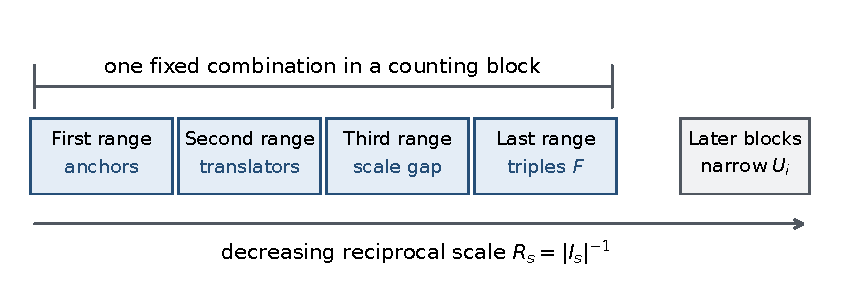
\includegraphics[width=\linewidth]{figures/counting-blocks.pdf}
 \caption{For one fixed choice of a current counting block, three
 core roles, and their future cover subsets, the four ranges shown
 remain after omitting the scale bins crossing the quartile cuts.
 Reciprocal scale decreases from left to right.  The ranges supply
 anchors, separated translators, a scale gap, and the set $F$.
 The selected future subsets lie in later counting blocks and have
 narrower neighborhoods.  These counting blocks are distinct from
 the consecutive $K$-depth blocks in Figure~\ref{fig:depth-blocks}.}
 \label{fig:counting-blocks}
\end{figure}

We will compare the $q|F|$ indexed outputs of the translated sets
$t_v+F$ with a cover of a common slab.  The next two steps build
covers of the future sumsets; the anchors will remove one factor
$M$ from the slab cover.  The scale margins will then show that
no cover box contains two of these outputs.

\paragraph{A small-growth scale without an exponential loss.}
Write $U_i$ and $\epsilon_i$ for the neighborhoods and widths of the
future block associated with $B_i$.  Subdividing each coefficient
interval and the scalar interval gives, for every integer $t\geq1$,
a cover of $U_i(t)$ by at most $(2t+1)^{d+1}$ translates of $U_i(1)$.
Consequently there is an odd integer
\[
 1\leq H_i\leq100(d+1)^2,
 \qquad |U_i(H_i+2)|\leq2|U_i(H_i)|.
\]
Otherwise growth by more than $2$ at each odd step would exceed
the displayed polynomial-in-$t$ bound by the time $t$ is a
sufficiently large absolute multiple of $(d+1)^2$.  The exponential
dependence on $d$ of the preliminary cover is used only for this
choice of $H_i$; it is not paid in the estimates below.

The translates $a+U_i(H_i)$, $a\in B_{i0}$, are disjoint.  An
intersection would put their difference in $U_i(2H_i)$, whose
shift index in the $\zeta$ lattice is $O((d+1)^2B)$ and whose
scalar width is at most $C(d+1)^2\nu R^\#$.  The reserves on
$Q$ and $\Sigma$ exclude this.  With
$Z_i=B_{i0}+U_i(H_i)$, the difference cover for $B_i-B_i$ gives
\[
 \begin{split}
 |Z_i-B_i|
 &\leq K_1M|U_i(H_i+2)|
 \leq2K_1M|U_i(H_i)|\\
 &\leq C(K_1L/\rho)|Z_i|.
 \end{split}
\]

\paragraph{The minimal-growth subset argument.}
Choose a nonempty $X_i\subseteq Z_i$ minimizing
$r_i=|X_i-B_i|/|X_i|$.  Then $r_i\leq CK_1L/\rho$.
We include the iteration argument, in the form used in
\cite{Petridis2012}.  For a finite family of translates
$C_0=\{c_1,\ldots,c_q\}$ let $X_{i,j}$ consist of the points $x\in X_i$
whose translate $x+c_j$ is not in any earlier $X_i+c_v$.
Thus $|X_i+C_0|=\sum_j|X_{i,j}|$.  Every point of
$(X_i\setminus X_{i,j})-B_i+c_j$ already belongs to an earlier
translate of $X_i-B_i$.  The new points contributed at step $j$
are therefore at most
\[
 \begin{split}
 |X_i-B_i|-|(X_i\setminus X_{i,j})-B_i|
 &\leq r_i|X_i|-r_i|X_i\setminus X_{i,j}|\\
 &=r_i|X_{i,j}|,
 \end{split}
\]
by minimality; the empty-complement case is included.  Summing and
then iterating with $C_0=-(m-1)B_i$ proves
\[
 |X_i-mB_i|\leq r_i^m|X_i|\qquad(m\geq1),
\]
where $mB_i$ denotes the $m$-fold sumset.

One anchor translate contains a portion $Y_i$ of $X_i$ of size at
least $|X_i|/M$, since there are at most $M$ anchors.  Its difference
set is contained in $U_i(2H_i)$.  If $\mathcal P$ is a packing of
$mB_i$ with distinct differences outside $U_i(2H_i)$, the translates
$Y_i-p$, $p\in\mathcal P$, are disjoint and belong to $X_i-mB_i$.
Hence
\[
 |\mathcal P|\leq r_i^m M.
\]
Maximal packings give covers by the same neighborhood.  We need
only $m=2,3$.

\paragraph{A slab cover with only two label-count factors.}
Put $r_0=CK_1L/\rho$, enlarging the absolute constant so that
$r_i\leq r_0$ for every role.  Consider the set of outputs in
$2B_1\times2B_2\times2B_3$ satisfying
\[
 \left|\sum_i\alpha_i x_i+36n\cdot\zeta\right|
       \leq2\nu R^\#
 \quad\text{for some }n\in\Z^d,\quad |n|_\infty\leq2B.
\]
Cover the first two sumsets by at most $r_0^2M$ translates each
of $U_i(2H_i)$.  Above a fixed pair of boxes, the possible third
coordinate lies in $2B_3$ intersected with a set of the form
\[
 c+\{n\cdot\zeta:|n|_\infty\leq C(d+1)^2B\}
       +[-C(d+1)^2\nu R^\#,C(d+1)^2\nu R^\#].
\]
Indeed substitute the first two coordinate boxes into the slab
relation and divide by $\alpha_3\in\{\pm1,\pm2,\pm3\}$.
The box shifts are $6n\cdot\zeta$ and the slab shifts are
$36n\cdot\zeta$, so the divided coefficients remain integral.
Their sizes have the stated bound.

Let $\mathcal P$ be a packing in this local third-coordinate set
outside $U_3(2H_3)$.  Then $B_{30}+\mathcal P\subseteq3B_3$ is
still such a packing.  For an equal anchor this is the definition
of $\mathcal P$.  For distinct anchors, a collision would express
their difference, modulo a reserved shift, with absolute value at
most $C(d+1)^2\nu R^\#$, contradicting their separation.  The
global $3B_3$ packing bound gives
\[
 |B_{30}|\,|\mathcal P|\leq r_0^3M,
 \qquad |\mathcal P|\leq Cr_0^3L/\rho.
\]
Covering the local third-coordinate set by a maximal packing shows
that the whole slab is covered by at most
\[
 C r_0^7(L/\rho)M^2
 \leq C K_1^7(L/\rho)^8M^2
\]
translates of $\prod_{i=1}^3U_i(2H_i)$.  The use of all the
separated anchors is what removes a third factor $M$.

\paragraph{All translated last-range triples are separated.}
For each chosen second-range triple $t_v$, translate $F$ by $t_v$.
All outputs belong to the preceding slab, by adding their annular
relations.  A cover box contains at most one output.  First, within
one translation, distinct members of $F$ differ in some label
coordinate.  Their last-range witnesses lie above every future
scale, so hereditary separation is stronger than membership of
that coordinate difference in $U_i(4H_i)$.

Next consider different translations, and let $R_{\mathrm{big}}$
be the larger of their two second-range scales.  The annular
residual of that triple has magnitude between
$\mu R_{\mathrm{big}}$ and $\nu R_{\mathrm{big}}$.  The sum of the
magnitudes of the other second-range residual and the two
last-range residuals is at most $\mu R_{\mathrm{big}}/10$, by
the factor-$\Gamma$ margins.  Thus the linear form of the output
difference, after a shift of index $O(B)$, has absolute value
between $9\mu R_{\mathrm{big}}/10$ and $2\nu R_{\mathrm{big}}$.
If the outputs lay in the same box, their coordinate differences
would be in $U_i(4H_i)$.  The total scalar error in the linear form
would then be at most
\[
 C(d+1)^2\nu\max_i R_{\mathrm{future},i}^+
 \leq\mu R_{\mathrm{big}}/10.
\]
All shifts still have index $O((d+1)^2B)\leq Q$.  We would obtain
a pure shift of magnitude between
$4\mu R_{\mathrm{big}}/5$ and $3\nu R_{\mathrm{big}}$, inside the
forbidden gap.  This proves the required separation.

The number $q|F|$ of outputs is consequently bounded by the slab
cover.  Cancelling $M^2$ gives
\[
 c\frac{\rho}{\delta\ell}\frac{\rho}{L}
       \leq C K_1^7(L/\rho)^8,
 \qquad \rho^{10}\leq C\delta\ell K_1^7L^9.
\]
Including the previously omitted case $\rho\leq C\delta\ell$,
a convenient uniform consequence is
\[
 \rho\leq C\ell K_1L\delta^{1/10}.
\]

\paragraph{Choice of the auxiliary powers.}
There are at most $4J_0^4K_1^3$ combinations.  Combining their
mass, the uncovered mass, and the nonfuture-pair mass, we obtain
\[
 \begin{split}
 M^{-2}\sum_{s:N_s\leq\delta M^2}N_s
 &\leq C\left(J_0\kappa+\sqrt{L\alpha}
          +\ell L J_0^4K_1^4\delta^{1/10}\right)\\
 &\leq C\left(\frac{L\kappa}{\alpha}
         +\sqrt{L\alpha}
         +\ell L^{29}\alpha^{-4}\kappa^{-24}\delta^{1/10}\right).
 \end{split}
\]
For sufficiently small absolute $\delta$, take
$\alpha=\delta^{1/1040}$ and $\kappa=\alpha^2$.
Then $\delta\leq\alpha/2$, and the three powers of $\delta$ on
the right are $1/1040$, $1/2080$, and
$1/10-52/1040=1/20$.  Since $L,\ell\geq1$, this proves the
asserted estimate.  For the remaining $\delta$, enlarge the absolute
constant and use the total-mass bound $LM^2$.
\end{proof}

\subsection{Application to the progression tests}

Fix a retained path point $x_*$, the height, all role types, the
frequency bands, and all amplitude bins in \eqref{eq:src-33}.
In each group define
\[
 M_i^G=|\mathcal A_i^G|\quad\text{for a core role},\qquad
 M_l^G=\sigma_l^{-2}
       \sum_{s:\ G\ \mathrm{used}}
                   \|S_{l,G,s}\|_{2,I_s}^2
       \quad\text{for a side role},
\]
and put $M'=\max_iM_i^G$.  We omit groups with no nonzero counts;
then $M'\geq1$.  In the side case this also follows directly from
$b_\Lambda\geq\sigma_l$ and Parseval at a nonzero use.

\begin{proposition}[Counts for the tested core tuples]
\label{prop:thin-count}
There is an absolute $p_0\in(0,1)$ such that, for the preceding
data and some
$L_0\leq P^C(1+\log(\nu/\mu))^C$, one has
\begin{equation*}
 \begin{split}
 \sum_sN_s^G
     &\leq L_0\min_{i\ne j}M_i^GM_j^G,\\
 \sum_s(N_s^G)^{p_0}
     &\leq P^C(1+\nu+\mu^{-1}+\Lambda)^C(M')^{2p_0}.
 \end{split}
 \tag{34}\label{eq:src-34}
\end{equation*}
All exponents are absolute.  They do not depend on the path,
the group, the horizontal dimension, or the number of depths.
\end{proposition}

\begin{proof}
Identify a label $a$ with its fixed value $\omega_a(x_*)$.
Different labels in one fixed role and type have distinct values
by \eqref{eq:src-25} with zero shift.  We first establish pair
determination.  In the four-core case, subtract the two frequency
tests for two incident tuples that have a given pair of labels in
common.  At a cost $O(\nu\max(R_s,R_t))$, the two remaining
frequencies solve the linear equations for $Q$ and $T$, modulo
the bounded shifts.  The inverse determinant divides by an integer
of magnitude at most $3$.  Separation \eqref{eq:src-25} forces the
two alternative labels in each remaining role to agree.  In the
three-core case, the single equation for $T_l$ similarly determines
the third core label from the other two, with a divisor of magnitude
at most $3$.  These conclusions hold across different scales,
because the separation threshold uses the larger reciprocal scale.
All shift differences and divisions fit the height reserve.

In addition, for any triple of core roles let $l'$ be the excluded
fourth role and put $\alpha_i'=i-l'$ on that triple.  The tests imply
\begin{equation*}
 c\mu R_s\leq
 \left|\sum_{i\ \mathrm{in\ the\ triple}}
                   \alpha_i'a_i+n\cdot\xi\right|
 \leq C\nu R_s,
 \qquad n\in\Z^{\dim\theta_z},\quad |n|_\infty\leq CB'_h.
 \tag{35}\label{eq:src-35}
\end{equation*}
For four cores this is $t'-l'q'$, using both bounds in
\eqref{eq:src-31}; for three cores it is precisely the nonzero
$T_l$ test.  Fixing a pair fixes the whole core tuple, and hence
the label values in this annulus.  The height-bin observation,
applied to those fixed values together with the coordinates of
$\xi$, bounds the number of scale occurrences by
$P^C(1+\log(\nu/\mu))^C$.  We use $L_0\geq1$ for a bound of
this form.  This proves the first count for any pair of core roles.

For a pair consisting of a core role and the side, fix the core
label and a scale.  The windows in \eqref{eq:src-32} associated
with different incident triples are disjoint.  If two windows
overlapped, their $Q$ values would be close modulo bounded shifts,
with error $O(\Lambda R_s)$.  Combining this with the two $T_l$
relations determines the two remaining core labels, again by a
two-by-two system with divisor at most $3$.  Since
$\nu,\Lambda\leq CU_0\ll\Xi$, separation forces those labels
to be identical.  Couple the fresh offset in all these windows.
Parseval for each offset, followed by expectation, shows that the
number of incident triples in the chosen side bin is at most
\[
 w_s=\sigma_l^{-2}\|S_{l,G,s}\|_{2,I_s}^2.
\]
This remains valid on any subset of scales after summing.  Summing
over the fixed core labels proves the first inequality of
\eqref{eq:src-34} for a core/side pair as well.

We now apply Lemma~\ref{lem:finite-sparse-count} with $M=M'$,
$L=L_0$, $d=\dim\theta_z$, and
\[
 \zeta=\xi/36.
\]
The fixed constants in \eqref{eq:src-35} may be absorbed by
decreasing $\mu$ and increasing $\nu$ by absolute factors.
The pair and side-budget hypotheses were just verified.  For
separation, note that
\[
 \frac{\xi}{36}=6^{\Delta-2}\frac{\vartheta}{L_h}.
\]
Thus the shifts in the finite lemma are among those of
\eqref{eq:src-25}, with
$Q=\lfloor E_h/6^{\Delta-2}\rfloor$ and
$\Sigma=\Xi/2$.  The choice of $A_0$ and
$B'_h=D_*^5E_{h-\Delta}$ ensures
$Q\geq C_{\mathrm{res}}(d+1)^2 CB'_h$.
Likewise $\Xi=D_*^{1000}$ and $\nu\leq CD_*^{250}$ ensure
the separation reserve, with room for the fixed annular constants.

Finally, any successful component contains a nonexceptional
primary, even when its representative is itself exceptional.
For that primary the pure-horizontal cases of \eqref{eq:src-23}
apply to every shift in the finite lemma: their rational heights
are smaller than $\mathcal H$.  They are either at most
$\mathcal T^{-1}/r_{v_b}$ or at least
$\mathcal T/r_{t_b}$.  Since
$U_0^{-1}\leq\mu\leq1\leq\nu\leq CU_0$ and the test scale lies
between these depth scales, the prescribed choice of $\mathcal T$
excludes the entire intermediate interval required by the
pure-shift hypothesis.  This checks every hypothesis of the
finite lemma, uniformly over the current group.

It follows that, for an absolute $c'>0$,
\begin{equation*}
 \sum_{s:\ N_s^G\leq\delta(M')^2}N_s^G
 \leq P^C(1+\nu+\mu^{-1}+\Lambda)^C
                 \delta^{c'}(M')^2
 \qquad(0<\delta\leq1).
 \tag{36}\label{eq:src-36}
\end{equation*}
For example, $c'=1/2080$ is admissible after changing the absolute
constants.  Indeed Lemma~\ref{lem:finite-sparse-count} gives the
stronger coefficient $C\ell L_0^{29}$; the dimension and the
logarithms in this expression fit the displayed budget.

Pair determination also gives $N_s^G\leq(M')^2$.  Choose
$p_0\in(0,1)$ with $1-p_0<c'$, for instance
$p_0=1-c'/2$.  On the set of scales with
\[
 2^{-j-1}(M')^2<N_s^G\leq2^{-j}(M')^2
\]
we may bound $(N_s^G)^{p_0}$ by
$[2^{j+1}/(M')^2]^{1-p_0}N_s^G$.  Sum this inequality and use
\eqref{eq:src-36} with $\delta=2^{-j}$.  The remaining geometric
series has ratio $2^{1-p_0-c'}<1$, and proves the second inequality
of \eqref{eq:src-34}.
\end{proof}

\subsection{Summing groups and amplitude bins}

\begin{proposition}[Powered estimate for the core terms]
\label{prop:core-estimate}
There are absolute $\varepsilon>0$ and $C_4<\infty$, with
$1-\varepsilon>2/3$, such that the terms containing at least three
core roles in the localized expansion of \eqref{eq:src-11} have
total contribution at most
\begin{equation*}
 C_q\eta^\varepsilon P^{C_4}|R|+O(e^{-k}|R|).
 \tag{37}\label{eq:src-37}
\end{equation*}
Here the original cell minimum is applied before the subadditive
estimates, and all numerical errors are estimated absolutely.
The constants are uniform in the finite depth range and the
retained attempt.  In particular $\varepsilon$ and $C_4$ can be
fixed before choosing how close $q$ is to $2$.
\end{proposition}

\begin{proof}
Set
\[
 p=1-\varepsilon=(1-\theta')+\theta'p_0,
\]
where $\theta'>0$ is a sufficiently small absolute number, to be
fixed below.  H\"older interpolation between the two inequalities
in \eqref{eq:src-34} gives, for any distinct roles $i,j$,
\[
 \sum_s(N_s^G)^p
 \leq
 (L_0M_i^GM_j^G)^{1-\theta'}
 \big[P^C(1+\nu+\mu^{-1}+\Lambda)^C
                     (M')^{2p_0}\big]^{\theta'}.
\]
Order the amplitude bins from largest to smallest, temporarily
calling their roles $1,2,3,4$, so that
$\sigma_1\geq\sigma_2\geq\sigma_3\geq\sigma_4$.
Use the pair $1,2$ in the first factor.  At least one of this pair
is a core role, because there is at most one side.

The path bounds \eqref{eq:src-28} and the side square budget give
\[
 \sum_G M_i^G\leq CP^C\sigma_i^{-2}
 \quad\text{in every role},\qquad
 \sum_G M_i^G\leq D_*
 \quad\text{in a core role}.
\]
Expand the maximum $M'$ into at most four choices of the role
attaining it.  The total exponent of the resulting product of
$M_i^G$ is $2p>1$.  For nonnegative sequences $m_i^G$ and
exponents $\beta_i\geq0$ with $\sum_i\beta_i\geq1$, one has
\[
 \sum_G\prod_i(m_i^G)^{\beta_i}
 \leq\prod_i\left(\sum_Gm_i^G\right)^{\beta_i}.
\]
Indeed normalize each nonzero sum to one, apply H\"older with
exponents $(\sum_i\beta_i)/\beta_i$, and use that the normalized
sequences have $\ell^{\sum\beta_i}$ norm at most one.  This proves
the needed group summation.

The largest size-to-count factor is $\sigma_4^{-2}$.  In the core
member of the first pair we may also use the count cap $D_*$.
If this member is role $2$, its factor
$\min(1,D_*\sigma_2^2)$ is bounded by the corresponding factor
with $\sigma_1$.  Multiplying by $(\prod_i\sigma_i)^p$ from
\eqref{eq:src-33}, the amplitude dependence is consequently at
most a $P^C$ factor times
\[
 \min(1,D_*\sigma_1^2)^{1-\theta'}
 \sigma_1^{p-2(1-\theta')}
 \sigma_2^{p-2(1-\theta')}
 \sigma_3^p\sigma_4^{p-4\theta'p_0}.
\]
Let the four displayed power exponents be $e_1,e_2,e_3,e_4$.
Their sum is zero, and their three preceding partial sums are
\[
 -1+\theta'(1+p_0),\qquad
 -2+2\theta'(1+p_0),\qquad
 -1+\theta'(1+3p_0).
\]
All are strictly negative when $\theta'$ is sufficiently small.
Writing $g_j=\log_2(\sigma_j/\sigma_{j+1})\geq0$, the remaining
power factor is $2^{\sum_{j=1}^3g_j(e_1+\cdots+e_j)}$.
Thus all three amplitude-gap sums are convergent geometric series.

Only a common shift of all the bins remains.  The retained upper
amplitude bound is $P^C$.  Below $\sigma_1=D_*^{-1/2}$ the
prefactor $\min(1,D_*\sigma_1^2)^{1-\theta'}$ decays geometrically;
above it there are only
$O(1+\log D_*+\log P)$ possible dyadic bins up to that upper
bound.  The common-shift cost is therefore polynomial in the
allowed logarithmic budgets.  There are only $24$ amplitude
orderings, so this completes the amplitude summation.

It remains to sum the frequency bands.  The first count loses
only powers of $1+\log(\nu/\mu)$.  The second count, after
interpolation, loses at most
$\mu^{-C\theta'}\nu^{C\theta'}\Lambda^{C\theta'}$.
The powered kernel factor in \eqref{eq:src-33} is
$\mu^p\nu^{-Lp}\Lambda^{-Lp}$.  First take $\theta'$ small
enough that $p-C\theta'>0$, and then take the fixed derivative
order $L$ sufficiently large.  The sums over dyadic
$0<\mu\leq1$ and $1\leq\nu,\Lambda<\infty$ converge, including
the logarithmic losses.  Extending the actual truncated ranges
to these ranges only increases the bound.  The number of heights,
types, role patterns, and retained leaves has an allowed
polynomial cost.  We have proved a bound $C_qP^{C_4}$ for the
path sum of the $p$th powers of all the principal core
contributions, keeping each $N_s^G$ inside its power.

To finish, let $\mathcal C_I$ be the sum of their absolute
principal contributions at a cell.  Subadditivity for $p<1$
and $\min(\eta,t)\leq\eta^{1-p}t^p$ give
\[
 \min(\eta,\mathcal C_I)
 \leq\eta^\varepsilon\mathcal C_I^p
 \leq\eta^\varepsilon
       \sum_{\mathrm{configurations}}
              (\text{principal contribution at }I)^p.
\]
Integrating the path estimate uses the exact identity
$\sum_I|I|F_I=\int_R\sum_{I\ni x_*}F_I\,dx_*$
for nonnegative cell data.  It gives
$C_q\eta^\varepsilon P^{C_4}|R|$.  The previously separated
absolute errors contribute $O(e^{-k}|R|)$, which proves
\eqref{eq:src-37}.  All polynomial degrees in the finite counting
lemma, and hence $p_0$, $\theta'$, $\varepsilon$, and $C_4$, are
absolute.  Taking $\theta'$ smaller if necessary gives
$p>2/3$ as required by the side estimates.
\end{proof}

\section{Parameter choice and completion of the proof}\label{sec:completion}
We finish Proposition~\ref{prop:normalized}.  Throughout this section all
collections of summation cells are finite and lie in the original $N$
depths.  Thus the defining constant $C_N(q)$ is finite, and every
application of it in Section~\ref{sec:sides} concerns precisely this
finite constant.

\subsection{One attempt and its restarts}
Fix one of the normalized base segments from Section~\ref{sec:base},
with root $R$, a tuple of increment levels, and one active pattern.
For the noninitial levels, its remaining quantity is
\[
 \sum_{I\text{ active}}|I|\min\{\eta,|H_I(z)|\},
 \qquad \eta=e^{-k^\theta},
\]
where $k$ is the later accuracy log and $\theta>0$ is fixed.
This is Equation~\eqref{eq:src-11}.
We explain explicitly how the stopping constructions preserve this
quantity.

Start an attempt at $R$.  Construct the main catalogs, color histories,
and ball filters, making the small marking-failure cuts from
Section~\ref{sec:localization}.  The objects needed on an unused branch
can be continued by inheritance and local refitting.  Next construct the
fixed first-match mode expansions and the linear side states of
Section~\ref{sec:linearization}.  Choose the branch offsets by the small
integrated error bound over all the pre-existing actual uses.  Finally
close the helper catalogs on the entire side states and the specified
histories.  A helper base is one such state, not an individual Fourier
mode or a choice of heights and amplitude bins.

All subsequent size and counting stops are imposed on these fixed
objects.  A stop removes original summands from the attempt; it does not
truncate or redefine a previously fixed stack function.  Partial path
counts and ancestor suprema are accumulated in increasing depth, and a
cell is stopped at their first threshold crossing.  Hence the retained
summands see only retained partial counts.  For the hull estimates of
Section~\ref{sec:sides}, include all potentially needed ancestors within
a block before imposing the common cuts.  The maximal functions remain
defined on the full retained hull cells, including portions below a cut.
Their joint caps are consequently valid on the sparse remainders used
in the proof of Equation~\eqref{eq:src-19}.
Large-frozen-complement flags are charged as powered errors within the
current attempt; only a first crossing of their accumulated power-cost
budget produces a restart root.

The integral bounds proved in the preceding sections permit each class
of stops to have arbitrarily small fixed relative root length by
increasing its threshold by a fixed factor.  The number of configurations
requiring the strong caps is a small overhead, which can be included in
those thresholds.  Polynomially many configurations in $P,k$ occur only
in the estimates already permitted a polynomial cost.  Choose these
thresholds together so that the union of first stopped cells has total
length at most, say, $|R|/4$.

At every stopped cell send the original base summands there and below
to a fresh attempt.  The original basic arguments and their inherited
lists remain the same.  Their normalized sizes hold on the new root;
the rolling basic projection bounds and the other local hypotheses hold
there as well.  Thus each attempt has the same estimates, uniformly in
its root and in the remaining number of depths.  The total length of
all roots in the resulting recursion is at most
\[
 |R|\sum_{n\ge0}4^{-n}=\tfrac43|R|.
\]
The construction terminates on a finite depth tree.  Equivalently, one
can prove the required bound by induction on the remaining depth, with
the displayed geometric root-length estimate.

\subsection{The estimate on retained cells}
Proposition~\ref{prop:localization} first gives the group decomposition
in Equation~\eqref{eq:src-14}.  In each coarse role the decomposition of
Section~\ref{sec:linearization} is a core plus a rolling and a linear
side, with a separately estimated physical error.  The basic rolling
$U$ role, if present, is always a side.

Terms with at least three core roles are estimated by
Proposition~\ref{prop:core-estimate}.  Terms with at least three side
factors have three square-size budgets, so they are summable at every
fixed power $p>2/3$ sufficiently close to one, with a polynomial cost in
$P,k$.  In a term with exactly two sides, replace its two core complements
by their whole current localized arguments.  The correction terms have
at least three sides.  Apply Lemma~\ref{lem:transfer} to the two whole
complements.  After transfer, replacing their basic coarse parts by the
full $Y$ arguments adds a third basic side; the remaining term has the
full complementary pair for which Section~\ref{sec:base} proves
smallness.  This is the pair-small main term in
Proposition~\ref{prop:side-estimate}.

The near-band defects are retained as their coupled band sums and
estimated at power one by Equation~\eqref{eq:src-19}.  Numerical errors
are also estimated at power one.  For all the other terms we use
\[
 \min\{\eta,a\}\le\eta^{1-p}a^p\qquad(a\ge0).
\]
The minimum is first applied to the sum at the original cell and then
split by subadditivity.  In particular no separate pair-smallness
assertion for an individual group is being used.  Put $p=1-\varepsilon$,
where $\varepsilon>0$ is fixed small enough for both the three-side
estimate and the interpolation in Section~\ref{sec:counting}.

The first term below collects the estimates taken at power
$p=1-\varepsilon$ and the smaller pair-small main term; the second is the
coupled near-band estimate at power one.  Combining
Equations~\eqref{eq:src-19} and~\eqref{eq:src-37} with the other side
estimates, and increasing one fixed exponent $C_4$ to include all powered
costs, gives on retained cells
\[
 C_q\left[
 \eta^{\varepsilon}P^{C_4}
 +(1+C_N)P^{-1/2}G_0(K+2)^{C_{19}(q-2)}
 \right]|R|+O(e^{-k}|R|).
\]
Fixed polynomial factors in $k$ can be retained here and absorbed into
the first term's power of $P$ once the parameters below are fixed.  The
main term after transfer, of size $\eta P^C|R|$, is also covered after
increasing $C_4$ and decreasing $\varepsilon$ if necessary.  The constant
$C_{19}$ is absolute.  Restarting as above changes this bound only by a
fixed factor.

\subsection{Order of the parameters}
For clarity, the two types of complexity used in the proof are listed
separately:
\begin{center}
\begin{tabular}{p{.28\linewidth}p{.31\linewidth}p{.30\linewidth}}
\toprule
Quantity & Allowed size & Role in the argument\\
\midrule
$D_{\mathrm{base}},D_{\mathrm m}$
 & $\log D\le C_q k^C$
 & Main columns, colors, helpers and their projection products.\\[3pt]
$D_*$ and the shift heights
 & $\log D_*\le C_q(1+k+P)^C$
 & Fixed linear modes, Fourier truncations and graph tests.\\[3pt]
$K$
 & $K\le C_q(1+k+P)^{C_5}$
 & Depth-block length after the mode and gap choices.\\[3pt]
$G_0$
 & $\exp(C_q(1+\log(2k))^C)$
 & Strong energy and stack overhead in Equations~\eqref{eq:src-17}--\eqref{eq:src-19}.\\
\bottomrule
\end{tabular}
\end{center}
Every exponent denoted by $C,C_4,C_5,C_{19}$ in this hierarchy has an
absolute upper bound before $q$ is chosen.  Constants such as $C_q$ may
depend on that later fixed choice.

Here is why the ordering is not circular.  Detection changes a power of
an accuracy log by an absolute amount; the dependence on $q$ from
clipping multiplies that log by a $q$-dependent constant.  Thus choose
the stagger exponent $A$ in Section~\ref{sec:base} and the small quality
exponent $\theta$ independently of $q$.  The main/helper catalogs have
polynomially many ranks and multiplicative count increments
$\exp(k^{C_2})$.  Their logarithms remain polynomial in $k$.
The number of masks and histories enters this recurrence logarithmically,
including the $P$ pad choices, because $\log P=O(k)$.  The tolerance in
Equation~\eqref{eq:src-13} includes $n_{r-1}^{-1/2}$, so summing a lower-rank
source does not require its full count as an additional error loss.
Choose the mismatch accuracy and the edge height after these count
bounds.  Color recourse bounds are uniform in that edge height.

The short-path construction then produces the larger mode budget.
Its Fourier cutoffs precede the height range, shift radii and horizontal
gap, and $K$ is chosen last among these quantities.  All their logarithms
are still polynomial in $P,k$.  The strong side estimate compresses only
main projection families; mode projections have already been incorporated
in Bessel rows.  The bad-density argument removes the large height
factor from its chain count.  Thus $G_0$ has the smaller size in the table,
whereas the top counts and core estimates may pay powers of $P$.
No later mode count is fed back into main/helper closure.

Now set $P=\lceil\eta^{-\alpha}\rceil$ for a fixed $\alpha>0$ to be
chosen.  For every such fixed choice and sufficiently large $k$,
$P$ dominates each fixed power of $k$ and $G_0=P^{o(1)}$.
First choose $2<q<3$ so close to two that
\[
 C_{19}C_5(q-2)<\tfrac18.
\]
After the finite overheads are combined, increasing the starting log
makes them at most $P^{1/8}$.  Hence
\[
 P^{-1/2}G_0(K+2)^{C_{19}(q-2)}\le C_qP^{-1/4}.
\]
Next choose $\alpha>0$ small enough that
$\alpha C_4<\varepsilon/2$, and impose the finitely many analogous
upper bounds coming from the other powered side costs.  Then
\[
 \eta^{\varepsilon}P^{C_4}\lesssim\eta^{\varepsilon/2},
 \qquad P^{-1/4}\le\eta^{\alpha/4}.
\]
Finally increase the starting log so that all earlier accuracy and
small-overhead requirements hold.  Since $\theta<1$, numerical errors
$e^{-k}$ are smaller than the resulting quality gain for large $k$.
We have therefore proved, for some fixed $c_*>0$, the bound
\[
 \sum_{I\text{ active}}|I|\min\{\eta,|H_I(z)|\}
 \le C_q\eta^{c_*}(1+C_N)|R|
\]
on every base segment and pattern.

\subsection{Summing the base expansion}
For later level $t$, there are $O(t)$ choices of the earlier increment
level and only a bounded number of slot patterns.  Each tuple uses
intersections of a bounded number of inheritance segments.  Their roots
have uniformly bounded total length by the reset packing in
Section~\ref{sec:base}; the further attempts just considered preserve
this property.  Thus the total coefficient of $1+C_N$ from the
noninitial tuples is bounded by a fixed multiple of
\[
 \sum_{t\ge12}t\exp(-c_*k_t^\theta),
 \qquad k_{t+1}=k_t^A.
\]
This series converges and tends to zero as $k_1$ tends to infinity.
The absolute errors $O(e^{-k_t})$ are summable with the same multiplicity.
The finitely many initial levels are bounded by the active-scale count
in Equation~\eqref{eq:src-10}; their cost is a finite constant depending
on the chosen starting logs but independent of $N$.

Given the small $c$ in Proposition~\ref{prop:normalized}, take $k_1$
large enough that the preceding coefficient of $C_N$ is at most $c$.
All remaining constants are included in $A$.  The base expansion is
first taken at a finite accuracy cutoff; on a fixed finite tree its
residual terms tend to zero by the staggered pair comparisons of
Section~\ref{sec:base}.  The uniform bounds just proved permit passage
to that limit.  We obtain the assertion of
Proposition~\ref{prop:normalized}.
Lemma~\ref{lem:outer} now proves Theorems~\ref{thm:local}
and~\ref{thm:main}.

\bibliographystyle{amsplain}
\bibliography{references}
\end{document}
